\chapter{Queueing theoretic model}\label{sec:queueing_section}

\section{Introduction}

One of the main outcomes of this research is the creation of a queueing network
model that consists of two queueing nodes and accepts two types of individuals.

\begin{figure}[H]
    \centering
    \begin{figure}[h]
    \centering
    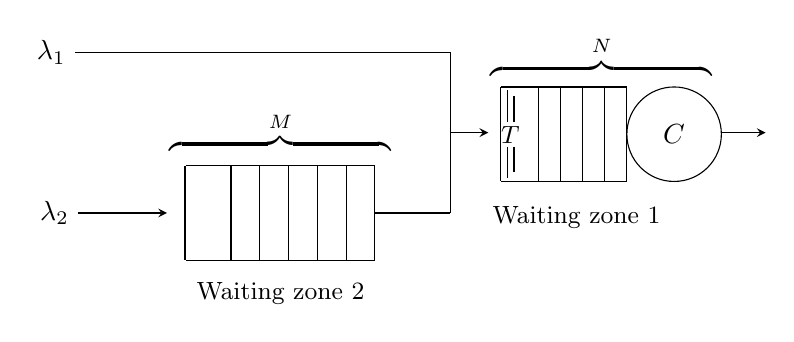
\begin{tikzpicture}[>=stealth, scale=0.8],
        % the rectangle of Queue 1
        \draw (0,0) -- ++(3cm,0) -- ++(0,-1.5cm) -- ++(-3cm,0);
        % The label above Queue 1 -> M
        \node[anchor=north] at (1.5cm, 1cm) {\(
            \overbrace{\qquad \qquad \qquad \qquad}^{M}
        \)};
        % The label below Queue 1 -> Waiting zone 2
        \node[anchor=north] at (1.5cm, -1.7cm) {\small{Waiting zone 2}};

        % the vertical lines in Queue 1
        \foreach \i in {1,...,5, 6.6}
        \draw (3cm-\i*13pt,0) -- +(0,-1.5cm);

        % % the circle in Queue 1
        % \draw (2.75,-0.75cm) circle [radius=0.75cm] node {\(0\)};

        % the rectangle in Queue 2
        \draw (5,1.25) -- ++(2cm,0) -- ++(0,-1.5cm) -- ++(-2cm,0);
        % the vertical lines in Queue 2
        \foreach \i in {1,...,4, 5.7}
        \draw (7cm-\i*10pt,1.25) -- +(0,-1.5cm);
        % The two vertical lines at the start of Queue 2
        \draw (7cm-54pt,1.2) -- +(0,-0.5cm);
        \draw (7cm-54pt,0.3) -- +(0,-0.5cm);
        \draw (7cm-51pt,1.1) -- +(0,-0.4cm);
        \draw (7cm-51pt,0.3) -- +(0,-0.4cm);

        % The label between the lines for T
        \node[anchor=north] at (5.15, 0.77 cm) {\small{\( T \)}};

        % The label above Queue 2 -> N
        \node[anchor=north] at (6.6cm, 2.2cm) {\(
            \overbrace{\qquad \qquad \qquad \qquad}^{N}
        \)};
        % The label below Queue 2 -> Waiting zone 1
        \node[anchor=north] at (6.2cm, -0.5cm) {\small{Waiting zone 1}};

        % the circle in Queue 2
        \draw (7.75,0.5) circle [radius=0.75cm] node {\(C\)};

        % Arrow line from Queue 2 outside
        \draw[->] (8.5,0.525) -- +(20pt,0);

        % Line from lambda_2 to Queue 1
        \draw[<-] (-0.3,-0.75) -- +(-40pt,0) node[left] {\( \lambda_2 \)};
        % First line (horizontal) after Queue 1
        \draw[-] (3,-0.75) -- +(34pt,0);
        % Second line (vertical) after Queue 1
        \draw (4.2, 0.525) -- (4.2, -0.75);

        % First line (horizontal) from lambda_1
        \draw (4.2, 1.8) -- +(-169.5pt,0) node[left] {\( \lambda_1 \)};
        % Second line (vertical) from lambda_1
        \draw (4.2, 1.8) -- (4.2, 0.525);
        % Arrow line to Queue 2
        \draw[->] (4.2, 0.525) -- (4.8, 0.525);
    \end{tikzpicture}
    \caption{A diagrammatic representation of the queueing network.
    The threshold \(T\) only applies to type 2 individuals.
    If the number of individuals in waiting zone 1 is greater than or equal to
    \(T\), only individuals of type 1 are accepted (at a rate \(\lambda_1\))
    and individuals of type 2 (arriving at a rate \(\lambda_2\)) are blocked in
    waiting zone 2.}
    \label{fig:diagram_of_queueing_system}
\end{figure}

    \caption{A diagrammatic representation of the queueing network.
    The threshold \(T\) only applies to type 2 individuals.
    If the number of individuals in node 1 is greater than or equal to
    \(T\), only individuals of type 1 are accepted (at a rate \(\lambda_1\))
    and individuals of type 2 (arriving at a rate \(\lambda_2\)) are blocked in
    node 2.}
    \label{fig:diagram_of_queueing_system}
\end{figure}

The model consists of two types of individuals; type 1 and type 2.
Type 1 individuals arrive instantly at node 1 and wait to receive their
service.
Type 2 individuals arrive at node 2 and wait there until they are
allowed to move to node 1.
They are allowed to proceed only when the number of
individuals in node 1 \textbf{and} in service is less than a
pre-determined threshold \(T\).
When the number of individuals is equal to or exceeds this threshold, all
type 2 individuals that arrive will stay \textit{blocked} in node 2
until the number of people in node 1 falls below \(T\).
This is shown diagrammatically in Figure~\ref{fig:diagram_of_queueing_system}.
The parameters of the described queueing model are:

\begin{itemize}
    \item \(\lambda_i\): The arrival rate of type \(i\) individuals where
    \(i\in\{1, 2\}\)
    \item \(\mu\): The service rate for individuals receiving service at
    node 1
    \item \(C\): The number of servers
    \item \(T\): The threshold at which individuals of the second type are
    blocked
    \item \(N\): The capacity of node 1 (i.e \(N=C + 
    \text{(Queue capacity)}\))
    \item \(M\): The capacity of node 2
\end{itemize}

Note that the parameters \(N\) and \(M\) are defined as the capacities of nodes
1 and 2 respectively.
In the case where these capacities are infinite, the queueing network can only
be modelled using the Discrete Event Simulation (DES) approach.
The Markov chain approach can only use \(N\) and \(M\) as artificial truncation
parameters to approximate the behaviour of the system.
In addition, when type \(1\) individuals arrive at node \(1\) and it is at full
capacity, they become lost from the system.
Similarly, when type \(2\) individuals arrive at node \(2\) and it is at full
capacity, they are also lost from the system.

In Section~\ref{sec:queueing_ems_ed_application} this queueing network will be
used to model the structure of an Emergency Department (ED) that receives
patients in ambulances from the Emergency Medical Services (EMS).
This chapter extends the concepts described in~\cite{panayides2023game} and
consists of the following sections:

\begin{itemize}
    \item Section~\ref{sec:discrete_event_simulation} gives an overview of
    the discrete event simulation model.
    \item Section~\ref{sec:markov_model} gives an overview of the Markov
    chain model.
    \item Section~\ref{sec:queueing_performance_measures} describes the Markov
    chain model is used to extract performance measures of the system.
    \item Section~\ref{sec:numeric_results_and_timings} presents some numerical
    results and timings experiments for the queueing network, along with
    a comparison between the DES and Markov chain approach.
    \item Section~\ref{sec:queueing_ems_ed_application} describes how the
    queueing network can be used to model the emergent behaviour between
    EDs and the EMS.
\end{itemize}




\subsection{Discrete Event Simulation}

Discrete Event Simulation (DES) is a method for modelling the behaviour of
real-world systems in which the system is made up of discrete events, each of
which has a certain duration~\cite{DESstewart}.
It can be used to understand complex situations in order to make predictions
and thus provide improvements~\cite{VinceGeraintBook}.
The three main approaches to building DES models are the activity scanning
approach, the event scheduling approach and the process interaction
approach~\cite{DESapproaches}.
Under the scope of this study only the event scheduling approach is considered.
This section describes the discrete event simulation (DES) model used to
represent the queueing network of Section~\ref{sec:queueing-section}.

In order to use DES on the queueing network described in
Figure~\ref{fig:diagram_of_queueing_system} an equivalent queueing network must
be constructed.
The current queueing network is a two-node queueing system that accepts two
types of individuals, where type 1 individuals arrive at waiting zone 1 and
type 2 individuals arrive at waiting zone 2.
The modification that is required revolves around the mechanisms of waiting
zone 2.
Waiting zone 2 is defined as a non-service node where there is only a queueing
space for individuals to wait there until they are allowed to waiting zone 1.
From an implementation perspective there is an equivalent system that can be
used where instead of a node with no service and queueing capacity \(M\), there
are \(M\) servers each serving with a service rate of \(0\) and no queueing
capacity, as shown in Figure \ref{fig:equivalent_diagram_of_queueing_system}.

\begin{figure}[h]
    \centering
    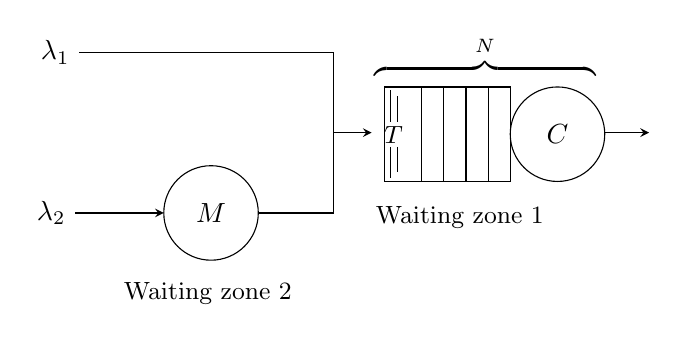
\begin{tikzpicture}[>=stealth, scale=0.8],

        % the circle in Queue 1
        \draw (2.25cm, -0.75cm) circle [radius=0.75cm] node {\(M\)};

        % The label below Queue 1 -> Waiting zone 2
        \node[anchor=north] at (2.2cm, -1.7cm) {\small{Waiting zone 2}};

        % the rectangle in Queue 2
        \draw (5, 1.25) -- ++(2cm, 0) -- ++(0, -1.5cm) -- ++(-2cm, 0);
        % the vertical lines in Queue 2
        \foreach \i in {1,...,4, 5.7}
        \draw (7cm-\i*10pt,1.25) -- +(0,-1.5cm);
        % The two vertical lines at the start of Queue 2
        \draw (7cm-54pt,1.2) -- +(0,-0.5cm);
        \draw (7cm-54pt,0.3) -- +(0,-0.5cm);
        \draw (7cm-51pt,1.1) -- +(0,-0.4cm);
        \draw (7cm-51pt,0.3) -- +(0,-0.4cm);

        % The label between the lines for T
        \node[anchor=north] at (5.15, 0.77 cm) {\small{\( T \)}};

        % The label above Queue 2 -> N
        \node[anchor=north] at (6.6cm, 2.2cm) {\(
            \overbrace{\qquad \qquad \qquad \qquad}^{N}
        \)};
        % The label below Queue 2 -> Waiting zone 1
        \node[anchor=north] at (6.2cm, -0.5cm) {\small{Waiting zone 1}};

        % the circle in Queue 2
        \draw (7.75,0.5) circle [radius=0.75cm] node {\(C\)};

        % Arrow line from Queue 2 outside
        \draw[->] (8.5,0.525) -- +(20pt,0);

        % Line from lambda_2 to Queue 1
        \draw[<-] (1.5,-0.75) -- +(-40pt,0) node[left] {\( \lambda_2 \)};
        % First line (horizontal) after Queue 1
        \draw[-] (3,-0.75) -- +(34pt,0);
        % Second line (vertical) after Queue 1
        \draw (4.2, 0.525) -- (4.2, -0.75);

        % First line (horizontal) from lambda_1
        \draw (4.2, 1.8) -- +(-115pt,0) node[left] {\( \lambda_1 \)};
        % Second line (vertical) from lambda_1
        \draw (4.2, 1.8) -- (4.2, 0.525);
        % Arrow line to Queue 2
        \draw[->] (4.2, 0.525) -- (4.8, 0.525);
    \end{tikzpicture}
    \caption{An equivalent model to the one described in
    Figure~\ref{fig:diagram_of_queueing_system}. The difference between the two
    diagrams is the formulation of waiting zone 2. The original diagram uses
    a node with no servers and a queueing capacity of \(M\) while this one uses
    \(M\) servers with no queueing capacity.}
    \label{fig:equivalent_diagram_of_queueing_system}
\end{figure}


The arrival times for both waiting zones are exponentially distributed with
mean \(\lambda_1\) and \(\lambda_2\) corresponding to type 1 and type 2
individuals respectively.
Waiting zone 1 has an exponentially distributed service time with rate \(\mu\),
a total of \(C\) servers and a queueing capacity of \(N - C\) (making the
overall capacity \(N\)). 
Waiting zone 2 has a deterministic service time of \(0\), a total of \(M\)
servers and a queueing capacity of \(M\).
Note here that, similar to Figure \ref{fig:diagram_of_queueing_system},
parameters \(N\) and \(M\) are used to approximate the real world system 
and in fact can be taken to be infinite in the DES.
Finally the routing parameter is defined as an array that probabilistically
routes individuals from all nodes to all other nodes.
For this particular system the routing parameter needs only to route individuals
from waiting zone 2 to waiting zone 1.

\begin{equation}
    \text{routing parameter} = \left[
    \begin{array}{cc}
        0 & 1 \\
        0 & 0
    \end{array}
    \right]
\end{equation}


\subsubsection{Implementation}
The python library \lstinline[style=pystyle]{ciw}~\cite{ciwpython, ciwarticle}
was used to implement the DES model.
The library treats queues as distinct nodes in the network where each node has
an arrival distribution, a service distribution, a number of available servers
and a queue capacity.
The following code can be used to generate a queueing network with two
queues and two types of individuals, where type 1 individuals arrive at node
2 (waiting zone 1) with an arrival rate of \lstinline[style=pystyle]{lambda_1}
and type 2 individuals arrive at node 1 (waiting zone 2) with an arrival rate of
\lstinline[style=pystyle]{lambda_2}.
Node 1 has a deterministic fixed service rate of \lstinline[style=pystyle]{0}
(since there is no service involved in the buffer centre) and node 2 has an
exponential service rate of \lstinline[style=pystyle]{mu}.

\begin{lstlisting}[style=pystyle]
>>> import ciw
>>> lambda_1 = 1.0
>>> lambda_2 = 2.0
>>> mu = 0.5
>>> num_of_servers = 3
>>> system_capacity = 10
>>> buffer_capacity = 5
>>> model = ciw.create_network(
...     arrival_distributions=[
...         ciw.dists.Exponential(lambda_2),
...         ciw.dists.Exponential(lambda_1)
...     ],
...     service_distributions=[
...         ciw.dists.Deterministic(0), ciw.dists.Exponential(mu)
...     ],
...     routing=[
...         [0.0, 1.0],
...         [0.0, 0.0]
...     ],
...     number_of_servers=[buffer_capacity, num_of_servers],
...     queue_capacities=[0, system_capacity - num_of_servers],
... )

\end{lstlisting}

As described earlier in Section~\ref{sec:queueing-section} and as shown in
Figure~\ref{fig:diagram_of_queueing_system}, type 1 individuals arrive at node 2
and exit the system after their service finishes, but type 2 individuals arrive
at node 1 and then proceed to node 2 after leaving node 1.
This logic is implemented in the queueing network using the
\lstinline[style=pystyle]{routing} parameter that consists of the routing
probabilities between different nodes.
For the current implementation the routing matrix is a \(2 \times 2\) array
that routes individuals from node 1 to node 2 with a probability of \(1.0\).
Furthermore, the server availability for nodes 1 and 2 are set to
the \lstinline[style=pystyle]{buffer_capacity} and
\lstinline[style=pystyle]{num_of_servers} respectively and the queue capacities
are set to \lstinline[style=pystyle]{0} and
\lstinline[style=pystyle]{system_capacity - num_of_servers}.
Note that for node 1 (i.e. waiting zone 2) queue capacity is set to 0 and its
number of servers is set to the buffer capacity.
From \lstinline[style=pystyle]{ciw}'s data records perspective this made more
sense since individuals are recorded as blocked this way.
If the queue capacity was non-zero, individuals could also have a waiting time
but no waiting should take place in node 1, only blockage.


\subsubsection{Custom node class}
Another specific feature of the particular model is that type 2 individuals
need to stay blocked in node 2 whenever the number of individuals in node 1
reaches a certain threshold \(T\).
This part of the queueing network is not as straightforward to implement as the
rest of the model.
\lstinline[style=pystyle]{Ciw} allows users to get more custom behaviour by
creating their own node class that inherits from the original one.
By inheriting the original \lstinline[style=pystyle]{ciw.Node} the general
behaviour of all nodes can be altered.


\begin{lstlisting}[style=pystyle]
>>> import numpy as np
>>> def build_custom_node(threshold=float("inf")):
...     """
...     Build a custom node to replace the default ciw.Node. Inherits from
...     the original ciw.Node class and replaces methods
...     release_blocked_individual and finish_service.
...     The methods are modified in such a way that all individuals that
...     are in the buffer space (node 1) stay blocked as long as the
...     number of individuals in the service area node (node 2) exceeds the
...     threshold.
...
...     Parameters
...     ----------
...     threshold : int, optional
...         The capacity threshold to be used by the method
...     Returns
...     -------
...     class
...         A custom node class that inherits from ciw.Node
...     """
...
...     class CustomNode(ciw.Node):
...         """
...         Overrides the default release_blocked_individual and
...         finish_service methods of the ciw.Node class
...         """
...
...         def __init__(self, id_, simulation):
...             """
...             Initializes the node with the given id and simulation using
...             the initialisation of ciw's Node object with the addition of
...             the threshold parameter.
...             """
...             super().__init__(id_, simulation)
...             self.simulation.threshold = threshold
...
...         def release_blocked_individual(self):
...             """
...             Releases an individual who becomes unblocked when
...             another individual is released:
...             - check if individual in node 2 and should stay blocked
...                 i.e. if the number of individuals in that
...                      node > threshold
...             - check if anyone is blocked by this node
...             - find the individual who has been blocked the longest
...             - remove that individual from blocked queue
...             - check if that individual had their service interrupted
...             - release that individual from their node
...             """
...             continue_blockage = (
...                 self.number_of_individuals >= threshold
...                 and self.id_number == 2
...             )
...             if (
...                 self.len_blocked_queue > 0
...                 and self.number_of_individuals < self.node_capacity
...                 and not continue_blockage
...             ):
...                 receiving_node = (
...                     self.simulation.nodes[self.blocked_queue[0][0]]
...                 )
...                 individual_to_receive_index = [
...                     ind.id_number
...                     for ind in receiving_node.all_individuals
...                 ].index(self.blocked_queue[0][1])
...                 individual_to_receive = (
...                     receiving_node.all_individuals[
...                         individual_to_receive_index
...                     ]
...                 )
...                 self.blocked_queue.pop(0)
...                 self.len_blocked_queue -= 1
...                 if individual_to_receive.interrupted:
...                     individual_to_receive.interrupted = False
...                     receiving_node.interrupted_individuals.remove(
...                         individual_to_receive
...                     )
...                     receiving_node.number_interrupted_individuals -= 1
...                 receiving_node.release(individual_to_receive_index, self)
...
...         def finish_service(self):
...             """
...             The next individual finishes service:
...             - finds the individual to finish service
...             - check if they need to change class
...             - find their next node
...             - release the individual if there is capacity at destination,
...                 otherwise cause blockage
...             - Note that blockage also occurs when we are at node 1 and
...                 the number of individuals on node 2 are more than the
...                 'threshold'
...             """
...             (
...                 next_individual,
...                 next_individual_index
...             ) = self.find_next_individual()
...             self.change_customer_class(next_individual)
...             next_node = self.next_node(next_individual)
...             next_individual.destination = next_node.id_number
...             if not np.isinf(self.c):
...                 next_individual.server.next_end_service_date=float("Inf")
...             blockage = (
...                 next_node.number_of_individuals >= threshold
...                 and self.id_number == 1
...             )
...             if (
...                 next_node.number_of_individuals < next_node.node_capacity
...             ) and not blockage:
...                 self.release(next_individual_index, next_node)
...             else:
...                 self.block_individual(next_individual, next_node)
...
...     return CustomNode

\end{lstlisting}

The class \lstinline[style=pystyle]{CustomNode} inherits from
\lstinline[style=pystyle]{ciw.Node} and changes two of the methods
(\lstinline[style=pystyle]{release_blocked_individual} and
\lstinline[style=pystyle]{finish_service}) so that the additional logic of the
threshold is incorporated.
In the \lstinline[style=pystyle]{release_blocked_individual} method an
additional check is added before releasing a potentially blocked individual from
node 1 to node 2.
This essentially checks whether the id of the node is 2 and
the number of individuals in it are more than or equal to the
\lstinline[style=pystyle]{threshold} so that it can accept a blocked individual.
Similarly \lstinline[style=pystyle]{finish_service} is called once an individual
finishes their service.
The additional check that was added checks whether the id of the node is 1 and
the number of individuals in the next node (i.e. node 2) is more than the
threshold, which would result in blockage.
Finally, the simulation object can be created and simulated for a specific
\lstinline[style=pystyle]{threshold} and \lstinline[style=pystyle]{runtime} by
running:

\begin{lstlisting}[style=pystyle]
>>> threshold = 4
>>> runtime = 1000
>>> custom_node = build_custom_node(threshold)
>>> simulation = ciw.Simulation(model, node_class=custom_node)
>>> simulation.simulate_until_max_time(runtime)

\end{lstlisting}




\section{Performance measures}\label{sec:queueing_performance_measures}
Using vector \(\pi\) there are numerous performance measures of the model that
can be calculated.
The following equations utilise \(\pi\) to get performance measures on the
average number of individuals in node 1 and in node 2:

\begin{itemize}
    \item Mean number of individuals in the entire system:
        \begin{equation}
            L_S = \sum_{i=1}^{|\pi|} \pi_i (u_i + v_i)
        \end{equation}
    \item Mean number of individuals in node 1:
        \begin{equation}
            L_1 = \sum_{i=1}^{|\pi|} \pi_i v_i
        \end{equation}
    \item Mean number of individuals in node 2:
        \begin{equation}
            L_2 = \sum_{i=1}^{|\pi|} \pi_i u_i
        \end{equation}
\end{itemize}

The python code for these functions may be obtained quite quickly using the set
of all states and the steady state probability.

\begin{lstlisting}[
    style=pystyle,
    caption={Code snippet for getting the set of all states and the steady
    state probabilities.},
    label={lst:set_of_all_states_and_steady_state_probabilities},
]
>>> import ambulance_game as abg
>>> import numpy as np
>>> all_states = abg.markov.build_states(
...     threshold=3 ,
...     system_capacity=4,
...     buffer_capacity=2
... )
>>> Q = abg.markov.get_transition_matrix(
...     lambda_1=1,
...     lambda_2=2,
...     mu=2,
...     num_of_servers=2,
...     threshold=3,
...     system_capacity=4,
...     buffer_capacity=2
... )
>>> pi = abg.markov.get_steady_state_algebraically(
...     Q, algebraic_function=np.linalg.lstsq
... )

\end{lstlisting}

Having the set of all states and the steady state probabilities, the mean
number of individuals in the system, in node 1 and in node 2 can be calculated
as shown in code snippets~\ref{lst:mean_number_of_individuals_in_system},
\ref{lst:mean_number_of_individuals_in_node_1}
and~\ref{lst:mean_number_of_individuals_in_node_2}.

\begin{lstlisting}[
    style=pystyle,
    caption={Code snippet for calculating the mean number of individuals in
    the system.},
    label={lst:mean_number_of_individuals_in_system},
]
>>> def get_mean_number_of_individuals_in_system(pi, states):
...     """Gets the mean number of individuals in the system
...     Parameters
...     ----------
...     pi : numpy.ndarray
...         steady state vector
...     states : list
...         list of tuples that contains all states
...     Returns
...     -------
...     float
...         Mean number of individuals in the whole model
...     """
...     states = np.array(states)
...     mean_inds_in_system = np.sum((states[:, 0] + states[:, 1]) * pi)
...     return mean_inds_in_system
>>>
>>> round(get_mean_number_of_individuals_in_system(pi, all_states), 10)
2.0872927227

\end{lstlisting}

\begin{lstlisting}[
    style=pystyle,
    caption={Code snippet for calculating the mean number of individuals in
    Node 1.},
    label={lst:mean_number_of_individuals_in_node_1},
]
>>> def get_mean_number_of_individuals_in_node_1(pi, states):
...     """Mean number of individuals in node 1
...     Parameters
...     ----------
...     pi : numpy.ndarray
...         steady state vector
...     states : list
...         list of tuples that contains all states
...     Returns
...     -------
...     float
...         Mean number of individuals
...     """
...     states = np.array(states)
...     mean_inds_in_node_1 = np.sum(states[:, 1] * pi)
...     return mean_inds_in_node_1
>>>
>>> round(get_mean_number_of_individuals_in_node_1(pi, all_states), 10)
1.8187129478

\end{lstlisting}

\begin{lstlisting}[
    style=pystyle,
    caption={Code snippet for calculating the mean number of individuals in
    Node 2.},
    label={lst:mean_number_of_individuals_in_node_2},
]
>>> def get_mean_number_of_individuals_in_node_2(pi, states):
...     """Mean number of class 2 individuals blocked
...     Parameters
...     ----------
...     pi : numpy.ndarray
...         steady state vector
...     states : list
...         list of tuples that contains all states
...     Returns
...     -------
...     float
...         Mean number of blocked class 2 individuals
...     """
...     states = np.array(states)
...     mean_blocked = np.sum(states[:, 0] * pi)
...     return mean_blocked
>>>
>>> round(get_mean_number_of_individuals_in_node_2(pi, all_states), 10)
0.2685797749

\end{lstlisting}


Consequently, there are some additional performance measures of interest that
are more complex to calculate.
Such performance measures are the mean waiting time in the system (for both
type 1 and type 2 individuals), the mean time blocked in node 2 (only
valid for type 2 individuals) and the proportion of individuals that wait in
node 1 within a predefined time target (for both types).
Under the scope of this study three approaches have been considered to calculate
these performance measures; a recursive algorithm, a direct approach and
a closed-form equation. 
Furthermore, different formulas arise for type 1 individuals and different
ones for type 2 individuals.


\section{Performance measures}\label{sec:queueing_performance_measures}
Using vector \(\pi\) there are numerous performance measures of the model that
can be calculated.
The following equations utilise \(\pi\) to get performance measures on the
average number of individuals in node 1 and in node 2:

\begin{itemize}
    \item Mean number of individuals in the entire system:
        \begin{equation}
            L_S = \sum_{i=1}^{|\pi|} \pi_i (u_i + v_i)
        \end{equation}
    \item Mean number of individuals in node 1:
        \begin{equation}
            L_1 = \sum_{i=1}^{|\pi|} \pi_i v_i
        \end{equation}
    \item Mean number of individuals in node 2:
        \begin{equation}
            L_2 = \sum_{i=1}^{|\pi|} \pi_i u_i
        \end{equation}
\end{itemize}

The python code for these functions may be obtained quite quickly using the set
of all states and the steady state probability.

\begin{lstlisting}[
    style=pystyle,
    caption={Code snippet for getting the set of all states and the steady
    state probabilities.},
    label={lst:set_of_all_states_and_steady_state_probabilities},
]
>>> import ambulance_game as abg
>>> import numpy as np
>>> all_states = abg.markov.build_states(
...     threshold=3 ,
...     system_capacity=4,
...     buffer_capacity=2
... )
>>> Q = abg.markov.get_transition_matrix(
...     lambda_1=1,
...     lambda_2=2,
...     mu=2,
...     num_of_servers=2,
...     threshold=3,
...     system_capacity=4,
...     buffer_capacity=2
... )
>>> pi = abg.markov.get_steady_state_algebraically(
...     Q, algebraic_function=np.linalg.lstsq
... )

\end{lstlisting}

Having the set of all states and the steady state probabilities, the mean
number of individuals in the system, in node 1 and in node 2 can be calculated
as shown in code snippets~\ref{lst:mean_number_of_individuals_in_system},
\ref{lst:mean_number_of_individuals_in_node_1}
and~\ref{lst:mean_number_of_individuals_in_node_2}.

\begin{lstlisting}[
    style=pystyle,
    caption={Code snippet for calculating the mean number of individuals in
    the system.},
    label={lst:mean_number_of_individuals_in_system},
]
>>> def get_mean_number_of_individuals_in_system(pi, states):
...     """Gets the mean number of individuals in the system
...     Parameters
...     ----------
...     pi : numpy.ndarray
...         steady state vector
...     states : list
...         list of tuples that contains all states
...     Returns
...     -------
...     float
...         Mean number of individuals in the whole model
...     """
...     states = np.array(states)
...     mean_inds_in_system = np.sum((states[:, 0] + states[:, 1]) * pi)
...     return mean_inds_in_system
>>>
>>> round(get_mean_number_of_individuals_in_system(pi, all_states), 10)
2.0872927227

\end{lstlisting}

\begin{lstlisting}[
    style=pystyle,
    caption={Code snippet for calculating the mean number of individuals in
    Node 1.},
    label={lst:mean_number_of_individuals_in_node_1},
]
>>> def get_mean_number_of_individuals_in_node_1(pi, states):
...     """Mean number of individuals in node 1
...     Parameters
...     ----------
...     pi : numpy.ndarray
...         steady state vector
...     states : list
...         list of tuples that contains all states
...     Returns
...     -------
...     float
...         Mean number of individuals
...     """
...     states = np.array(states)
...     mean_inds_in_node_1 = np.sum(states[:, 1] * pi)
...     return mean_inds_in_node_1
>>>
>>> round(get_mean_number_of_individuals_in_node_1(pi, all_states), 10)
1.8187129478

\end{lstlisting}

\begin{lstlisting}[
    style=pystyle,
    caption={Code snippet for calculating the mean number of individuals in
    Node 2.},
    label={lst:mean_number_of_individuals_in_node_2},
]
>>> def get_mean_number_of_individuals_in_node_2(pi, states):
...     """Mean number of class 2 individuals blocked
...     Parameters
...     ----------
...     pi : numpy.ndarray
...         steady state vector
...     states : list
...         list of tuples that contains all states
...     Returns
...     -------
...     float
...         Mean number of blocked class 2 individuals
...     """
...     states = np.array(states)
...     mean_blocked = np.sum(states[:, 0] * pi)
...     return mean_blocked
>>>
>>> round(get_mean_number_of_individuals_in_node_2(pi, all_states), 10)
0.2685797749

\end{lstlisting}


Consequently, there are some additional performance measures of interest that
are more complex to calculate.
Such performance measures are the mean waiting time in the system (for both
type 1 and type 2 individuals), the mean time blocked in node 2 (only
valid for type 2 individuals) and the proportion of individuals that wait in
node 1 within a predefined time target (for both types).
Under the scope of this study three approaches have been considered to calculate
these performance measures; a recursive algorithm, a direct approach and
a closed-form equation. 
Furthermore, different formulas arise for type 1 individuals and different
ones for type 2 individuals.


\section{Performance measures}\label{sec:queueing_performance_measures}
Using vector \(\pi\) there are numerous performance measures of the model that
can be calculated.
The following equations utilise \(\pi\) to get performance measures on the
average number of individuals in node 1 and in node 2:

\begin{itemize}
    \item Mean number of individuals in the entire system:
        \begin{equation}
            L_S = \sum_{i=1}^{|\pi|} \pi_i (u_i + v_i)
        \end{equation}
    \item Mean number of individuals in node 1:
        \begin{equation}
            L_1 = \sum_{i=1}^{|\pi|} \pi_i v_i
        \end{equation}
    \item Mean number of individuals in node 2:
        \begin{equation}
            L_2 = \sum_{i=1}^{|\pi|} \pi_i u_i
        \end{equation}
\end{itemize}

The python code for these functions may be obtained quite quickly using the set
of all states and the steady state probability.

\begin{lstlisting}[
    style=pystyle,
    caption={Code snippet for getting the set of all states and the steady
    state probabilities.},
    label={lst:set_of_all_states_and_steady_state_probabilities},
]
>>> import ambulance_game as abg
>>> import numpy as np
>>> all_states = abg.markov.build_states(
...     threshold=3 ,
...     system_capacity=4,
...     buffer_capacity=2
... )
>>> Q = abg.markov.get_transition_matrix(
...     lambda_1=1,
...     lambda_2=2,
...     mu=2,
...     num_of_servers=2,
...     threshold=3,
...     system_capacity=4,
...     buffer_capacity=2
... )
>>> pi = abg.markov.get_steady_state_algebraically(
...     Q, algebraic_function=np.linalg.lstsq
... )

\end{lstlisting}

Having the set of all states and the steady state probabilities, the mean
number of individuals in the system, in node 1 and in node 2 can be calculated
as shown in code snippets~\ref{lst:mean_number_of_individuals_in_system},
\ref{lst:mean_number_of_individuals_in_node_1}
and~\ref{lst:mean_number_of_individuals_in_node_2}.

\begin{lstlisting}[
    style=pystyle,
    caption={Code snippet for calculating the mean number of individuals in
    the system.},
    label={lst:mean_number_of_individuals_in_system},
]
>>> def get_mean_number_of_individuals_in_system(pi, states):
...     """Gets the mean number of individuals in the system
...     Parameters
...     ----------
...     pi : numpy.ndarray
...         steady state vector
...     states : list
...         list of tuples that contains all states
...     Returns
...     -------
...     float
...         Mean number of individuals in the whole model
...     """
...     states = np.array(states)
...     mean_inds_in_system = np.sum((states[:, 0] + states[:, 1]) * pi)
...     return mean_inds_in_system
>>>
>>> round(get_mean_number_of_individuals_in_system(pi, all_states), 10)
2.0872927227

\end{lstlisting}

\begin{lstlisting}[
    style=pystyle,
    caption={Code snippet for calculating the mean number of individuals in
    Node 1.},
    label={lst:mean_number_of_individuals_in_node_1},
]
>>> def get_mean_number_of_individuals_in_node_1(pi, states):
...     """Mean number of individuals in node 1
...     Parameters
...     ----------
...     pi : numpy.ndarray
...         steady state vector
...     states : list
...         list of tuples that contains all states
...     Returns
...     -------
...     float
...         Mean number of individuals
...     """
...     states = np.array(states)
...     mean_inds_in_node_1 = np.sum(states[:, 1] * pi)
...     return mean_inds_in_node_1
>>>
>>> round(get_mean_number_of_individuals_in_node_1(pi, all_states), 10)
1.8187129478

\end{lstlisting}

\begin{lstlisting}[
    style=pystyle,
    caption={Code snippet for calculating the mean number of individuals in
    Node 2.},
    label={lst:mean_number_of_individuals_in_node_2},
]
>>> def get_mean_number_of_individuals_in_node_2(pi, states):
...     """Mean number of class 2 individuals blocked
...     Parameters
...     ----------
...     pi : numpy.ndarray
...         steady state vector
...     states : list
...         list of tuples that contains all states
...     Returns
...     -------
...     float
...         Mean number of blocked class 2 individuals
...     """
...     states = np.array(states)
...     mean_blocked = np.sum(states[:, 0] * pi)
...     return mean_blocked
>>>
>>> round(get_mean_number_of_individuals_in_node_2(pi, all_states), 10)
0.2685797749

\end{lstlisting}


Consequently, there are some additional performance measures of interest that
are more complex to calculate.
Such performance measures are the mean waiting time in the system (for both
type 1 and type 2 individuals), the mean time blocked in node 2 (only
valid for type 2 individuals) and the proportion of individuals that wait in
node 1 within a predefined time target (for both types).
Under the scope of this study three approaches have been considered to calculate
these performance measures; a recursive algorithm, a direct approach and
a closed-form equation. 
Furthermore, different formulas arise for type 1 individuals and different
ones for type 2 individuals.


\input{chapters/03_queueing_model/03_performance_measures/01_waiting_time/main.tex}

\input{chapters/03_queueing_model/03_performance_measures/02_blocking_time/main.tex}

\input{chapters/03_queueing_model/03_performance_measures/03_proportion_of_individuals_within_time/main.tex}

\section{Performance measures}\label{sec:queueing_performance_measures}
Using vector \(\pi\) there are numerous performance measures of the model that
can be calculated.
The following equations utilise \(\pi\) to get performance measures on the
average number of individuals in node 1 and in node 2:

\begin{itemize}
    \item Mean number of individuals in the entire system:
        \begin{equation}
            L_S = \sum_{i=1}^{|\pi|} \pi_i (u_i + v_i)
        \end{equation}
    \item Mean number of individuals in node 1:
        \begin{equation}
            L_1 = \sum_{i=1}^{|\pi|} \pi_i v_i
        \end{equation}
    \item Mean number of individuals in node 2:
        \begin{equation}
            L_2 = \sum_{i=1}^{|\pi|} \pi_i u_i
        \end{equation}
\end{itemize}

The python code for these functions may be obtained quite quickly using the set
of all states and the steady state probability.

\begin{lstlisting}[
    style=pystyle,
    caption={Code snippet for getting the set of all states and the steady
    state probabilities.},
    label={lst:set_of_all_states_and_steady_state_probabilities},
]
>>> import ambulance_game as abg
>>> import numpy as np
>>> all_states = abg.markov.build_states(
...     threshold=3 ,
...     system_capacity=4,
...     buffer_capacity=2
... )
>>> Q = abg.markov.get_transition_matrix(
...     lambda_1=1,
...     lambda_2=2,
...     mu=2,
...     num_of_servers=2,
...     threshold=3,
...     system_capacity=4,
...     buffer_capacity=2
... )
>>> pi = abg.markov.get_steady_state_algebraically(
...     Q, algebraic_function=np.linalg.lstsq
... )

\end{lstlisting}

Having the set of all states and the steady state probabilities, the mean
number of individuals in the system, in node 1 and in node 2 can be calculated
as shown in code snippets~\ref{lst:mean_number_of_individuals_in_system},
\ref{lst:mean_number_of_individuals_in_node_1}
and~\ref{lst:mean_number_of_individuals_in_node_2}.

\begin{lstlisting}[
    style=pystyle,
    caption={Code snippet for calculating the mean number of individuals in
    the system.},
    label={lst:mean_number_of_individuals_in_system},
]
>>> def get_mean_number_of_individuals_in_system(pi, states):
...     """Gets the mean number of individuals in the system
...     Parameters
...     ----------
...     pi : numpy.ndarray
...         steady state vector
...     states : list
...         list of tuples that contains all states
...     Returns
...     -------
...     float
...         Mean number of individuals in the whole model
...     """
...     states = np.array(states)
...     mean_inds_in_system = np.sum((states[:, 0] + states[:, 1]) * pi)
...     return mean_inds_in_system
>>>
>>> round(get_mean_number_of_individuals_in_system(pi, all_states), 10)
2.0872927227

\end{lstlisting}

\begin{lstlisting}[
    style=pystyle,
    caption={Code snippet for calculating the mean number of individuals in
    Node 1.},
    label={lst:mean_number_of_individuals_in_node_1},
]
>>> def get_mean_number_of_individuals_in_node_1(pi, states):
...     """Mean number of individuals in node 1
...     Parameters
...     ----------
...     pi : numpy.ndarray
...         steady state vector
...     states : list
...         list of tuples that contains all states
...     Returns
...     -------
...     float
...         Mean number of individuals
...     """
...     states = np.array(states)
...     mean_inds_in_node_1 = np.sum(states[:, 1] * pi)
...     return mean_inds_in_node_1
>>>
>>> round(get_mean_number_of_individuals_in_node_1(pi, all_states), 10)
1.8187129478

\end{lstlisting}

\begin{lstlisting}[
    style=pystyle,
    caption={Code snippet for calculating the mean number of individuals in
    Node 2.},
    label={lst:mean_number_of_individuals_in_node_2},
]
>>> def get_mean_number_of_individuals_in_node_2(pi, states):
...     """Mean number of class 2 individuals blocked
...     Parameters
...     ----------
...     pi : numpy.ndarray
...         steady state vector
...     states : list
...         list of tuples that contains all states
...     Returns
...     -------
...     float
...         Mean number of blocked class 2 individuals
...     """
...     states = np.array(states)
...     mean_blocked = np.sum(states[:, 0] * pi)
...     return mean_blocked
>>>
>>> round(get_mean_number_of_individuals_in_node_2(pi, all_states), 10)
0.2685797749

\end{lstlisting}


Consequently, there are some additional performance measures of interest that
are more complex to calculate.
Such performance measures are the mean waiting time in the system (for both
type 1 and type 2 individuals), the mean time blocked in node 2 (only
valid for type 2 individuals) and the proportion of individuals that wait in
node 1 within a predefined time target (for both types).
Under the scope of this study three approaches have been considered to calculate
these performance measures; a recursive algorithm, a direct approach and
a closed-form equation. 
Furthermore, different formulas arise for type 1 individuals and different
ones for type 2 individuals.


\input{chapters/03_queueing_model/03_performance_measures/01_waiting_time/main.tex}

\input{chapters/03_queueing_model/03_performance_measures/02_blocking_time/main.tex}

\input{chapters/03_queueing_model/03_performance_measures/03_proportion_of_individuals_within_time/main.tex}

\section{Performance measures}\label{sec:queueing_performance_measures}
Using vector \(\pi\) there are numerous performance measures of the model that
can be calculated.
The following equations utilise \(\pi\) to get performance measures on the
average number of individuals in node 1 and in node 2:

\begin{itemize}
    \item Mean number of individuals in the entire system:
        \begin{equation}
            L_S = \sum_{i=1}^{|\pi|} \pi_i (u_i + v_i)
        \end{equation}
    \item Mean number of individuals in node 1:
        \begin{equation}
            L_1 = \sum_{i=1}^{|\pi|} \pi_i v_i
        \end{equation}
    \item Mean number of individuals in node 2:
        \begin{equation}
            L_2 = \sum_{i=1}^{|\pi|} \pi_i u_i
        \end{equation}
\end{itemize}

The python code for these functions may be obtained quite quickly using the set
of all states and the steady state probability.

\begin{lstlisting}[
    style=pystyle,
    caption={Code snippet for getting the set of all states and the steady
    state probabilities.},
    label={lst:set_of_all_states_and_steady_state_probabilities},
]
>>> import ambulance_game as abg
>>> import numpy as np
>>> all_states = abg.markov.build_states(
...     threshold=3 ,
...     system_capacity=4,
...     buffer_capacity=2
... )
>>> Q = abg.markov.get_transition_matrix(
...     lambda_1=1,
...     lambda_2=2,
...     mu=2,
...     num_of_servers=2,
...     threshold=3,
...     system_capacity=4,
...     buffer_capacity=2
... )
>>> pi = abg.markov.get_steady_state_algebraically(
...     Q, algebraic_function=np.linalg.lstsq
... )

\end{lstlisting}

Having the set of all states and the steady state probabilities, the mean
number of individuals in the system, in node 1 and in node 2 can be calculated
as shown in code snippets~\ref{lst:mean_number_of_individuals_in_system},
\ref{lst:mean_number_of_individuals_in_node_1}
and~\ref{lst:mean_number_of_individuals_in_node_2}.

\begin{lstlisting}[
    style=pystyle,
    caption={Code snippet for calculating the mean number of individuals in
    the system.},
    label={lst:mean_number_of_individuals_in_system},
]
>>> def get_mean_number_of_individuals_in_system(pi, states):
...     """Gets the mean number of individuals in the system
...     Parameters
...     ----------
...     pi : numpy.ndarray
...         steady state vector
...     states : list
...         list of tuples that contains all states
...     Returns
...     -------
...     float
...         Mean number of individuals in the whole model
...     """
...     states = np.array(states)
...     mean_inds_in_system = np.sum((states[:, 0] + states[:, 1]) * pi)
...     return mean_inds_in_system
>>>
>>> round(get_mean_number_of_individuals_in_system(pi, all_states), 10)
2.0872927227

\end{lstlisting}

\begin{lstlisting}[
    style=pystyle,
    caption={Code snippet for calculating the mean number of individuals in
    Node 1.},
    label={lst:mean_number_of_individuals_in_node_1},
]
>>> def get_mean_number_of_individuals_in_node_1(pi, states):
...     """Mean number of individuals in node 1
...     Parameters
...     ----------
...     pi : numpy.ndarray
...         steady state vector
...     states : list
...         list of tuples that contains all states
...     Returns
...     -------
...     float
...         Mean number of individuals
...     """
...     states = np.array(states)
...     mean_inds_in_node_1 = np.sum(states[:, 1] * pi)
...     return mean_inds_in_node_1
>>>
>>> round(get_mean_number_of_individuals_in_node_1(pi, all_states), 10)
1.8187129478

\end{lstlisting}

\begin{lstlisting}[
    style=pystyle,
    caption={Code snippet for calculating the mean number of individuals in
    Node 2.},
    label={lst:mean_number_of_individuals_in_node_2},
]
>>> def get_mean_number_of_individuals_in_node_2(pi, states):
...     """Mean number of class 2 individuals blocked
...     Parameters
...     ----------
...     pi : numpy.ndarray
...         steady state vector
...     states : list
...         list of tuples that contains all states
...     Returns
...     -------
...     float
...         Mean number of blocked class 2 individuals
...     """
...     states = np.array(states)
...     mean_blocked = np.sum(states[:, 0] * pi)
...     return mean_blocked
>>>
>>> round(get_mean_number_of_individuals_in_node_2(pi, all_states), 10)
0.2685797749

\end{lstlisting}


Consequently, there are some additional performance measures of interest that
are more complex to calculate.
Such performance measures are the mean waiting time in the system (for both
type 1 and type 2 individuals), the mean time blocked in node 2 (only
valid for type 2 individuals) and the proportion of individuals that wait in
node 1 within a predefined time target (for both types).
Under the scope of this study three approaches have been considered to calculate
these performance measures; a recursive algorithm, a direct approach and
a closed-form equation. 
Furthermore, different formulas arise for type 1 individuals and different
ones for type 2 individuals.


\input{chapters/03_queueing_model/03_performance_measures/01_waiting_time/main.tex}

\input{chapters/03_queueing_model/03_performance_measures/02_blocking_time/main.tex}

\input{chapters/03_queueing_model/03_performance_measures/03_proportion_of_individuals_within_time/main.tex}

\section{Performance measures}\label{sec:queueing_performance_measures}
Using vector \(\pi\) there are numerous performance measures of the model that
can be calculated.
The following equations utilise \(\pi\) to get performance measures on the
average number of individuals in node 1 and in node 2:

\begin{itemize}
    \item Mean number of individuals in the entire system:
        \begin{equation}
            L_S = \sum_{i=1}^{|\pi|} \pi_i (u_i + v_i)
        \end{equation}
    \item Mean number of individuals in node 1:
        \begin{equation}
            L_1 = \sum_{i=1}^{|\pi|} \pi_i v_i
        \end{equation}
    \item Mean number of individuals in node 2:
        \begin{equation}
            L_2 = \sum_{i=1}^{|\pi|} \pi_i u_i
        \end{equation}
\end{itemize}

The python code for these functions may be obtained quite quickly using the set
of all states and the steady state probability.

\begin{lstlisting}[
    style=pystyle,
    caption={Code snippet for getting the set of all states and the steady
    state probabilities.},
    label={lst:set_of_all_states_and_steady_state_probabilities},
]
>>> import ambulance_game as abg
>>> import numpy as np
>>> all_states = abg.markov.build_states(
...     threshold=3 ,
...     system_capacity=4,
...     buffer_capacity=2
... )
>>> Q = abg.markov.get_transition_matrix(
...     lambda_1=1,
...     lambda_2=2,
...     mu=2,
...     num_of_servers=2,
...     threshold=3,
...     system_capacity=4,
...     buffer_capacity=2
... )
>>> pi = abg.markov.get_steady_state_algebraically(
...     Q, algebraic_function=np.linalg.lstsq
... )

\end{lstlisting}

Having the set of all states and the steady state probabilities, the mean
number of individuals in the system, in node 1 and in node 2 can be calculated
as shown in code snippets~\ref{lst:mean_number_of_individuals_in_system},
\ref{lst:mean_number_of_individuals_in_node_1}
and~\ref{lst:mean_number_of_individuals_in_node_2}.

\begin{lstlisting}[
    style=pystyle,
    caption={Code snippet for calculating the mean number of individuals in
    the system.},
    label={lst:mean_number_of_individuals_in_system},
]
>>> def get_mean_number_of_individuals_in_system(pi, states):
...     """Gets the mean number of individuals in the system
...     Parameters
...     ----------
...     pi : numpy.ndarray
...         steady state vector
...     states : list
...         list of tuples that contains all states
...     Returns
...     -------
...     float
...         Mean number of individuals in the whole model
...     """
...     states = np.array(states)
...     mean_inds_in_system = np.sum((states[:, 0] + states[:, 1]) * pi)
...     return mean_inds_in_system
>>>
>>> round(get_mean_number_of_individuals_in_system(pi, all_states), 10)
2.0872927227

\end{lstlisting}

\begin{lstlisting}[
    style=pystyle,
    caption={Code snippet for calculating the mean number of individuals in
    Node 1.},
    label={lst:mean_number_of_individuals_in_node_1},
]
>>> def get_mean_number_of_individuals_in_node_1(pi, states):
...     """Mean number of individuals in node 1
...     Parameters
...     ----------
...     pi : numpy.ndarray
...         steady state vector
...     states : list
...         list of tuples that contains all states
...     Returns
...     -------
...     float
...         Mean number of individuals
...     """
...     states = np.array(states)
...     mean_inds_in_node_1 = np.sum(states[:, 1] * pi)
...     return mean_inds_in_node_1
>>>
>>> round(get_mean_number_of_individuals_in_node_1(pi, all_states), 10)
1.8187129478

\end{lstlisting}

\begin{lstlisting}[
    style=pystyle,
    caption={Code snippet for calculating the mean number of individuals in
    Node 2.},
    label={lst:mean_number_of_individuals_in_node_2},
]
>>> def get_mean_number_of_individuals_in_node_2(pi, states):
...     """Mean number of class 2 individuals blocked
...     Parameters
...     ----------
...     pi : numpy.ndarray
...         steady state vector
...     states : list
...         list of tuples that contains all states
...     Returns
...     -------
...     float
...         Mean number of blocked class 2 individuals
...     """
...     states = np.array(states)
...     mean_blocked = np.sum(states[:, 0] * pi)
...     return mean_blocked
>>>
>>> round(get_mean_number_of_individuals_in_node_2(pi, all_states), 10)
0.2685797749

\end{lstlisting}


Consequently, there are some additional performance measures of interest that
are more complex to calculate.
Such performance measures are the mean waiting time in the system (for both
type 1 and type 2 individuals), the mean time blocked in node 2 (only
valid for type 2 individuals) and the proportion of individuals that wait in
node 1 within a predefined time target (for both types).
Under the scope of this study three approaches have been considered to calculate
these performance measures; a recursive algorithm, a direct approach and
a closed-form equation. 
Furthermore, different formulas arise for type 1 individuals and different
ones for type 2 individuals.


\section{Performance measures}\label{sec:queueing_performance_measures}
Using vector \(\pi\) there are numerous performance measures of the model that
can be calculated.
The following equations utilise \(\pi\) to get performance measures on the
average number of individuals in node 1 and in node 2:

\begin{itemize}
    \item Mean number of individuals in the entire system:
        \begin{equation}
            L_S = \sum_{i=1}^{|\pi|} \pi_i (u_i + v_i)
        \end{equation}
    \item Mean number of individuals in node 1:
        \begin{equation}
            L_1 = \sum_{i=1}^{|\pi|} \pi_i v_i
        \end{equation}
    \item Mean number of individuals in node 2:
        \begin{equation}
            L_2 = \sum_{i=1}^{|\pi|} \pi_i u_i
        \end{equation}
\end{itemize}

The python code for these functions may be obtained quite quickly using the set
of all states and the steady state probability.

\begin{lstlisting}[
    style=pystyle,
    caption={Code snippet for getting the set of all states and the steady
    state probabilities.},
    label={lst:set_of_all_states_and_steady_state_probabilities},
]
>>> import ambulance_game as abg
>>> import numpy as np
>>> all_states = abg.markov.build_states(
...     threshold=3 ,
...     system_capacity=4,
...     buffer_capacity=2
... )
>>> Q = abg.markov.get_transition_matrix(
...     lambda_1=1,
...     lambda_2=2,
...     mu=2,
...     num_of_servers=2,
...     threshold=3,
...     system_capacity=4,
...     buffer_capacity=2
... )
>>> pi = abg.markov.get_steady_state_algebraically(
...     Q, algebraic_function=np.linalg.lstsq
... )

\end{lstlisting}

Having the set of all states and the steady state probabilities, the mean
number of individuals in the system, in node 1 and in node 2 can be calculated
as shown in code snippets~\ref{lst:mean_number_of_individuals_in_system},
\ref{lst:mean_number_of_individuals_in_node_1}
and~\ref{lst:mean_number_of_individuals_in_node_2}.

\begin{lstlisting}[
    style=pystyle,
    caption={Code snippet for calculating the mean number of individuals in
    the system.},
    label={lst:mean_number_of_individuals_in_system},
]
>>> def get_mean_number_of_individuals_in_system(pi, states):
...     """Gets the mean number of individuals in the system
...     Parameters
...     ----------
...     pi : numpy.ndarray
...         steady state vector
...     states : list
...         list of tuples that contains all states
...     Returns
...     -------
...     float
...         Mean number of individuals in the whole model
...     """
...     states = np.array(states)
...     mean_inds_in_system = np.sum((states[:, 0] + states[:, 1]) * pi)
...     return mean_inds_in_system
>>>
>>> round(get_mean_number_of_individuals_in_system(pi, all_states), 10)
2.0872927227

\end{lstlisting}

\begin{lstlisting}[
    style=pystyle,
    caption={Code snippet for calculating the mean number of individuals in
    Node 1.},
    label={lst:mean_number_of_individuals_in_node_1},
]
>>> def get_mean_number_of_individuals_in_node_1(pi, states):
...     """Mean number of individuals in node 1
...     Parameters
...     ----------
...     pi : numpy.ndarray
...         steady state vector
...     states : list
...         list of tuples that contains all states
...     Returns
...     -------
...     float
...         Mean number of individuals
...     """
...     states = np.array(states)
...     mean_inds_in_node_1 = np.sum(states[:, 1] * pi)
...     return mean_inds_in_node_1
>>>
>>> round(get_mean_number_of_individuals_in_node_1(pi, all_states), 10)
1.8187129478

\end{lstlisting}

\begin{lstlisting}[
    style=pystyle,
    caption={Code snippet for calculating the mean number of individuals in
    Node 2.},
    label={lst:mean_number_of_individuals_in_node_2},
]
>>> def get_mean_number_of_individuals_in_node_2(pi, states):
...     """Mean number of class 2 individuals blocked
...     Parameters
...     ----------
...     pi : numpy.ndarray
...         steady state vector
...     states : list
...         list of tuples that contains all states
...     Returns
...     -------
...     float
...         Mean number of blocked class 2 individuals
...     """
...     states = np.array(states)
...     mean_blocked = np.sum(states[:, 0] * pi)
...     return mean_blocked
>>>
>>> round(get_mean_number_of_individuals_in_node_2(pi, all_states), 10)
0.2685797749

\end{lstlisting}


Consequently, there are some additional performance measures of interest that
are more complex to calculate.
Such performance measures are the mean waiting time in the system (for both
type 1 and type 2 individuals), the mean time blocked in node 2 (only
valid for type 2 individuals) and the proportion of individuals that wait in
node 1 within a predefined time target (for both types).
Under the scope of this study three approaches have been considered to calculate
these performance measures; a recursive algorithm, a direct approach and
a closed-form equation. 
Furthermore, different formulas arise for type 1 individuals and different
ones for type 2 individuals.


\input{chapters/03_queueing_model/03_performance_measures/01_waiting_time/main.tex}

\input{chapters/03_queueing_model/03_performance_measures/02_blocking_time/main.tex}

\input{chapters/03_queueing_model/03_performance_measures/03_proportion_of_individuals_within_time/main.tex}

\section{Performance measures}\label{sec:queueing_performance_measures}
Using vector \(\pi\) there are numerous performance measures of the model that
can be calculated.
The following equations utilise \(\pi\) to get performance measures on the
average number of individuals in node 1 and in node 2:

\begin{itemize}
    \item Mean number of individuals in the entire system:
        \begin{equation}
            L_S = \sum_{i=1}^{|\pi|} \pi_i (u_i + v_i)
        \end{equation}
    \item Mean number of individuals in node 1:
        \begin{equation}
            L_1 = \sum_{i=1}^{|\pi|} \pi_i v_i
        \end{equation}
    \item Mean number of individuals in node 2:
        \begin{equation}
            L_2 = \sum_{i=1}^{|\pi|} \pi_i u_i
        \end{equation}
\end{itemize}

The python code for these functions may be obtained quite quickly using the set
of all states and the steady state probability.

\begin{lstlisting}[
    style=pystyle,
    caption={Code snippet for getting the set of all states and the steady
    state probabilities.},
    label={lst:set_of_all_states_and_steady_state_probabilities},
]
>>> import ambulance_game as abg
>>> import numpy as np
>>> all_states = abg.markov.build_states(
...     threshold=3 ,
...     system_capacity=4,
...     buffer_capacity=2
... )
>>> Q = abg.markov.get_transition_matrix(
...     lambda_1=1,
...     lambda_2=2,
...     mu=2,
...     num_of_servers=2,
...     threshold=3,
...     system_capacity=4,
...     buffer_capacity=2
... )
>>> pi = abg.markov.get_steady_state_algebraically(
...     Q, algebraic_function=np.linalg.lstsq
... )

\end{lstlisting}

Having the set of all states and the steady state probabilities, the mean
number of individuals in the system, in node 1 and in node 2 can be calculated
as shown in code snippets~\ref{lst:mean_number_of_individuals_in_system},
\ref{lst:mean_number_of_individuals_in_node_1}
and~\ref{lst:mean_number_of_individuals_in_node_2}.

\begin{lstlisting}[
    style=pystyle,
    caption={Code snippet for calculating the mean number of individuals in
    the system.},
    label={lst:mean_number_of_individuals_in_system},
]
>>> def get_mean_number_of_individuals_in_system(pi, states):
...     """Gets the mean number of individuals in the system
...     Parameters
...     ----------
...     pi : numpy.ndarray
...         steady state vector
...     states : list
...         list of tuples that contains all states
...     Returns
...     -------
...     float
...         Mean number of individuals in the whole model
...     """
...     states = np.array(states)
...     mean_inds_in_system = np.sum((states[:, 0] + states[:, 1]) * pi)
...     return mean_inds_in_system
>>>
>>> round(get_mean_number_of_individuals_in_system(pi, all_states), 10)
2.0872927227

\end{lstlisting}

\begin{lstlisting}[
    style=pystyle,
    caption={Code snippet for calculating the mean number of individuals in
    Node 1.},
    label={lst:mean_number_of_individuals_in_node_1},
]
>>> def get_mean_number_of_individuals_in_node_1(pi, states):
...     """Mean number of individuals in node 1
...     Parameters
...     ----------
...     pi : numpy.ndarray
...         steady state vector
...     states : list
...         list of tuples that contains all states
...     Returns
...     -------
...     float
...         Mean number of individuals
...     """
...     states = np.array(states)
...     mean_inds_in_node_1 = np.sum(states[:, 1] * pi)
...     return mean_inds_in_node_1
>>>
>>> round(get_mean_number_of_individuals_in_node_1(pi, all_states), 10)
1.8187129478

\end{lstlisting}

\begin{lstlisting}[
    style=pystyle,
    caption={Code snippet for calculating the mean number of individuals in
    Node 2.},
    label={lst:mean_number_of_individuals_in_node_2},
]
>>> def get_mean_number_of_individuals_in_node_2(pi, states):
...     """Mean number of class 2 individuals blocked
...     Parameters
...     ----------
...     pi : numpy.ndarray
...         steady state vector
...     states : list
...         list of tuples that contains all states
...     Returns
...     -------
...     float
...         Mean number of blocked class 2 individuals
...     """
...     states = np.array(states)
...     mean_blocked = np.sum(states[:, 0] * pi)
...     return mean_blocked
>>>
>>> round(get_mean_number_of_individuals_in_node_2(pi, all_states), 10)
0.2685797749

\end{lstlisting}


Consequently, there are some additional performance measures of interest that
are more complex to calculate.
Such performance measures are the mean waiting time in the system (for both
type 1 and type 2 individuals), the mean time blocked in node 2 (only
valid for type 2 individuals) and the proportion of individuals that wait in
node 1 within a predefined time target (for both types).
Under the scope of this study three approaches have been considered to calculate
these performance measures; a recursive algorithm, a direct approach and
a closed-form equation. 
Furthermore, different formulas arise for type 1 individuals and different
ones for type 2 individuals.


\input{chapters/03_queueing_model/03_performance_measures/01_waiting_time/main.tex}

\input{chapters/03_queueing_model/03_performance_measures/02_blocking_time/main.tex}

\input{chapters/03_queueing_model/03_performance_measures/03_proportion_of_individuals_within_time/main.tex}

\section{Performance measures}\label{sec:queueing_performance_measures}
Using vector \(\pi\) there are numerous performance measures of the model that
can be calculated.
The following equations utilise \(\pi\) to get performance measures on the
average number of individuals in node 1 and in node 2:

\begin{itemize}
    \item Mean number of individuals in the entire system:
        \begin{equation}
            L_S = \sum_{i=1}^{|\pi|} \pi_i (u_i + v_i)
        \end{equation}
    \item Mean number of individuals in node 1:
        \begin{equation}
            L_1 = \sum_{i=1}^{|\pi|} \pi_i v_i
        \end{equation}
    \item Mean number of individuals in node 2:
        \begin{equation}
            L_2 = \sum_{i=1}^{|\pi|} \pi_i u_i
        \end{equation}
\end{itemize}

The python code for these functions may be obtained quite quickly using the set
of all states and the steady state probability.

\begin{lstlisting}[
    style=pystyle,
    caption={Code snippet for getting the set of all states and the steady
    state probabilities.},
    label={lst:set_of_all_states_and_steady_state_probabilities},
]
>>> import ambulance_game as abg
>>> import numpy as np
>>> all_states = abg.markov.build_states(
...     threshold=3 ,
...     system_capacity=4,
...     buffer_capacity=2
... )
>>> Q = abg.markov.get_transition_matrix(
...     lambda_1=1,
...     lambda_2=2,
...     mu=2,
...     num_of_servers=2,
...     threshold=3,
...     system_capacity=4,
...     buffer_capacity=2
... )
>>> pi = abg.markov.get_steady_state_algebraically(
...     Q, algebraic_function=np.linalg.lstsq
... )

\end{lstlisting}

Having the set of all states and the steady state probabilities, the mean
number of individuals in the system, in node 1 and in node 2 can be calculated
as shown in code snippets~\ref{lst:mean_number_of_individuals_in_system},
\ref{lst:mean_number_of_individuals_in_node_1}
and~\ref{lst:mean_number_of_individuals_in_node_2}.

\begin{lstlisting}[
    style=pystyle,
    caption={Code snippet for calculating the mean number of individuals in
    the system.},
    label={lst:mean_number_of_individuals_in_system},
]
>>> def get_mean_number_of_individuals_in_system(pi, states):
...     """Gets the mean number of individuals in the system
...     Parameters
...     ----------
...     pi : numpy.ndarray
...         steady state vector
...     states : list
...         list of tuples that contains all states
...     Returns
...     -------
...     float
...         Mean number of individuals in the whole model
...     """
...     states = np.array(states)
...     mean_inds_in_system = np.sum((states[:, 0] + states[:, 1]) * pi)
...     return mean_inds_in_system
>>>
>>> round(get_mean_number_of_individuals_in_system(pi, all_states), 10)
2.0872927227

\end{lstlisting}

\begin{lstlisting}[
    style=pystyle,
    caption={Code snippet for calculating the mean number of individuals in
    Node 1.},
    label={lst:mean_number_of_individuals_in_node_1},
]
>>> def get_mean_number_of_individuals_in_node_1(pi, states):
...     """Mean number of individuals in node 1
...     Parameters
...     ----------
...     pi : numpy.ndarray
...         steady state vector
...     states : list
...         list of tuples that contains all states
...     Returns
...     -------
...     float
...         Mean number of individuals
...     """
...     states = np.array(states)
...     mean_inds_in_node_1 = np.sum(states[:, 1] * pi)
...     return mean_inds_in_node_1
>>>
>>> round(get_mean_number_of_individuals_in_node_1(pi, all_states), 10)
1.8187129478

\end{lstlisting}

\begin{lstlisting}[
    style=pystyle,
    caption={Code snippet for calculating the mean number of individuals in
    Node 2.},
    label={lst:mean_number_of_individuals_in_node_2},
]
>>> def get_mean_number_of_individuals_in_node_2(pi, states):
...     """Mean number of class 2 individuals blocked
...     Parameters
...     ----------
...     pi : numpy.ndarray
...         steady state vector
...     states : list
...         list of tuples that contains all states
...     Returns
...     -------
...     float
...         Mean number of blocked class 2 individuals
...     """
...     states = np.array(states)
...     mean_blocked = np.sum(states[:, 0] * pi)
...     return mean_blocked
>>>
>>> round(get_mean_number_of_individuals_in_node_2(pi, all_states), 10)
0.2685797749

\end{lstlisting}


Consequently, there are some additional performance measures of interest that
are more complex to calculate.
Such performance measures are the mean waiting time in the system (for both
type 1 and type 2 individuals), the mean time blocked in node 2 (only
valid for type 2 individuals) and the proportion of individuals that wait in
node 1 within a predefined time target (for both types).
Under the scope of this study three approaches have been considered to calculate
these performance measures; a recursive algorithm, a direct approach and
a closed-form equation. 
Furthermore, different formulas arise for type 1 individuals and different
ones for type 2 individuals.


\input{chapters/03_queueing_model/03_performance_measures/01_waiting_time/main.tex}

\input{chapters/03_queueing_model/03_performance_measures/02_blocking_time/main.tex}

\input{chapters/03_queueing_model/03_performance_measures/03_proportion_of_individuals_within_time/main.tex}

\section{Performance measures}\label{sec:queueing_performance_measures}
Using vector \(\pi\) there are numerous performance measures of the model that
can be calculated.
The following equations utilise \(\pi\) to get performance measures on the
average number of individuals in node 1 and in node 2:

\begin{itemize}
    \item Mean number of individuals in the entire system:
        \begin{equation}
            L_S = \sum_{i=1}^{|\pi|} \pi_i (u_i + v_i)
        \end{equation}
    \item Mean number of individuals in node 1:
        \begin{equation}
            L_1 = \sum_{i=1}^{|\pi|} \pi_i v_i
        \end{equation}
    \item Mean number of individuals in node 2:
        \begin{equation}
            L_2 = \sum_{i=1}^{|\pi|} \pi_i u_i
        \end{equation}
\end{itemize}

The python code for these functions may be obtained quite quickly using the set
of all states and the steady state probability.

\begin{lstlisting}[
    style=pystyle,
    caption={Code snippet for getting the set of all states and the steady
    state probabilities.},
    label={lst:set_of_all_states_and_steady_state_probabilities},
]
>>> import ambulance_game as abg
>>> import numpy as np
>>> all_states = abg.markov.build_states(
...     threshold=3 ,
...     system_capacity=4,
...     buffer_capacity=2
... )
>>> Q = abg.markov.get_transition_matrix(
...     lambda_1=1,
...     lambda_2=2,
...     mu=2,
...     num_of_servers=2,
...     threshold=3,
...     system_capacity=4,
...     buffer_capacity=2
... )
>>> pi = abg.markov.get_steady_state_algebraically(
...     Q, algebraic_function=np.linalg.lstsq
... )

\end{lstlisting}

Having the set of all states and the steady state probabilities, the mean
number of individuals in the system, in node 1 and in node 2 can be calculated
as shown in code snippets~\ref{lst:mean_number_of_individuals_in_system},
\ref{lst:mean_number_of_individuals_in_node_1}
and~\ref{lst:mean_number_of_individuals_in_node_2}.

\begin{lstlisting}[
    style=pystyle,
    caption={Code snippet for calculating the mean number of individuals in
    the system.},
    label={lst:mean_number_of_individuals_in_system},
]
>>> def get_mean_number_of_individuals_in_system(pi, states):
...     """Gets the mean number of individuals in the system
...     Parameters
...     ----------
...     pi : numpy.ndarray
...         steady state vector
...     states : list
...         list of tuples that contains all states
...     Returns
...     -------
...     float
...         Mean number of individuals in the whole model
...     """
...     states = np.array(states)
...     mean_inds_in_system = np.sum((states[:, 0] + states[:, 1]) * pi)
...     return mean_inds_in_system
>>>
>>> round(get_mean_number_of_individuals_in_system(pi, all_states), 10)
2.0872927227

\end{lstlisting}

\begin{lstlisting}[
    style=pystyle,
    caption={Code snippet for calculating the mean number of individuals in
    Node 1.},
    label={lst:mean_number_of_individuals_in_node_1},
]
>>> def get_mean_number_of_individuals_in_node_1(pi, states):
...     """Mean number of individuals in node 1
...     Parameters
...     ----------
...     pi : numpy.ndarray
...         steady state vector
...     states : list
...         list of tuples that contains all states
...     Returns
...     -------
...     float
...         Mean number of individuals
...     """
...     states = np.array(states)
...     mean_inds_in_node_1 = np.sum(states[:, 1] * pi)
...     return mean_inds_in_node_1
>>>
>>> round(get_mean_number_of_individuals_in_node_1(pi, all_states), 10)
1.8187129478

\end{lstlisting}

\begin{lstlisting}[
    style=pystyle,
    caption={Code snippet for calculating the mean number of individuals in
    Node 2.},
    label={lst:mean_number_of_individuals_in_node_2},
]
>>> def get_mean_number_of_individuals_in_node_2(pi, states):
...     """Mean number of class 2 individuals blocked
...     Parameters
...     ----------
...     pi : numpy.ndarray
...         steady state vector
...     states : list
...         list of tuples that contains all states
...     Returns
...     -------
...     float
...         Mean number of blocked class 2 individuals
...     """
...     states = np.array(states)
...     mean_blocked = np.sum(states[:, 0] * pi)
...     return mean_blocked
>>>
>>> round(get_mean_number_of_individuals_in_node_2(pi, all_states), 10)
0.2685797749

\end{lstlisting}


Consequently, there are some additional performance measures of interest that
are more complex to calculate.
Such performance measures are the mean waiting time in the system (for both
type 1 and type 2 individuals), the mean time blocked in node 2 (only
valid for type 2 individuals) and the proportion of individuals that wait in
node 1 within a predefined time target (for both types).
Under the scope of this study three approaches have been considered to calculate
these performance measures; a recursive algorithm, a direct approach and
a closed-form equation. 
Furthermore, different formulas arise for type 1 individuals and different
ones for type 2 individuals.


\section{Performance measures}\label{sec:queueing_performance_measures}
Using vector \(\pi\) there are numerous performance measures of the model that
can be calculated.
The following equations utilise \(\pi\) to get performance measures on the
average number of individuals in node 1 and in node 2:

\begin{itemize}
    \item Mean number of individuals in the entire system:
        \begin{equation}
            L_S = \sum_{i=1}^{|\pi|} \pi_i (u_i + v_i)
        \end{equation}
    \item Mean number of individuals in node 1:
        \begin{equation}
            L_1 = \sum_{i=1}^{|\pi|} \pi_i v_i
        \end{equation}
    \item Mean number of individuals in node 2:
        \begin{equation}
            L_2 = \sum_{i=1}^{|\pi|} \pi_i u_i
        \end{equation}
\end{itemize}

The python code for these functions may be obtained quite quickly using the set
of all states and the steady state probability.

\begin{lstlisting}[
    style=pystyle,
    caption={Code snippet for getting the set of all states and the steady
    state probabilities.},
    label={lst:set_of_all_states_and_steady_state_probabilities},
]
>>> import ambulance_game as abg
>>> import numpy as np
>>> all_states = abg.markov.build_states(
...     threshold=3 ,
...     system_capacity=4,
...     buffer_capacity=2
... )
>>> Q = abg.markov.get_transition_matrix(
...     lambda_1=1,
...     lambda_2=2,
...     mu=2,
...     num_of_servers=2,
...     threshold=3,
...     system_capacity=4,
...     buffer_capacity=2
... )
>>> pi = abg.markov.get_steady_state_algebraically(
...     Q, algebraic_function=np.linalg.lstsq
... )

\end{lstlisting}

Having the set of all states and the steady state probabilities, the mean
number of individuals in the system, in node 1 and in node 2 can be calculated
as shown in code snippets~\ref{lst:mean_number_of_individuals_in_system},
\ref{lst:mean_number_of_individuals_in_node_1}
and~\ref{lst:mean_number_of_individuals_in_node_2}.

\begin{lstlisting}[
    style=pystyle,
    caption={Code snippet for calculating the mean number of individuals in
    the system.},
    label={lst:mean_number_of_individuals_in_system},
]
>>> def get_mean_number_of_individuals_in_system(pi, states):
...     """Gets the mean number of individuals in the system
...     Parameters
...     ----------
...     pi : numpy.ndarray
...         steady state vector
...     states : list
...         list of tuples that contains all states
...     Returns
...     -------
...     float
...         Mean number of individuals in the whole model
...     """
...     states = np.array(states)
...     mean_inds_in_system = np.sum((states[:, 0] + states[:, 1]) * pi)
...     return mean_inds_in_system
>>>
>>> round(get_mean_number_of_individuals_in_system(pi, all_states), 10)
2.0872927227

\end{lstlisting}

\begin{lstlisting}[
    style=pystyle,
    caption={Code snippet for calculating the mean number of individuals in
    Node 1.},
    label={lst:mean_number_of_individuals_in_node_1},
]
>>> def get_mean_number_of_individuals_in_node_1(pi, states):
...     """Mean number of individuals in node 1
...     Parameters
...     ----------
...     pi : numpy.ndarray
...         steady state vector
...     states : list
...         list of tuples that contains all states
...     Returns
...     -------
...     float
...         Mean number of individuals
...     """
...     states = np.array(states)
...     mean_inds_in_node_1 = np.sum(states[:, 1] * pi)
...     return mean_inds_in_node_1
>>>
>>> round(get_mean_number_of_individuals_in_node_1(pi, all_states), 10)
1.8187129478

\end{lstlisting}

\begin{lstlisting}[
    style=pystyle,
    caption={Code snippet for calculating the mean number of individuals in
    Node 2.},
    label={lst:mean_number_of_individuals_in_node_2},
]
>>> def get_mean_number_of_individuals_in_node_2(pi, states):
...     """Mean number of class 2 individuals blocked
...     Parameters
...     ----------
...     pi : numpy.ndarray
...         steady state vector
...     states : list
...         list of tuples that contains all states
...     Returns
...     -------
...     float
...         Mean number of blocked class 2 individuals
...     """
...     states = np.array(states)
...     mean_blocked = np.sum(states[:, 0] * pi)
...     return mean_blocked
>>>
>>> round(get_mean_number_of_individuals_in_node_2(pi, all_states), 10)
0.2685797749

\end{lstlisting}


Consequently, there are some additional performance measures of interest that
are more complex to calculate.
Such performance measures are the mean waiting time in the system (for both
type 1 and type 2 individuals), the mean time blocked in node 2 (only
valid for type 2 individuals) and the proportion of individuals that wait in
node 1 within a predefined time target (for both types).
Under the scope of this study three approaches have been considered to calculate
these performance measures; a recursive algorithm, a direct approach and
a closed-form equation. 
Furthermore, different formulas arise for type 1 individuals and different
ones for type 2 individuals.


\input{chapters/03_queueing_model/03_performance_measures/01_waiting_time/main.tex}

\input{chapters/03_queueing_model/03_performance_measures/02_blocking_time/main.tex}

\input{chapters/03_queueing_model/03_performance_measures/03_proportion_of_individuals_within_time/main.tex}

\section{Performance measures}\label{sec:queueing_performance_measures}
Using vector \(\pi\) there are numerous performance measures of the model that
can be calculated.
The following equations utilise \(\pi\) to get performance measures on the
average number of individuals in node 1 and in node 2:

\begin{itemize}
    \item Mean number of individuals in the entire system:
        \begin{equation}
            L_S = \sum_{i=1}^{|\pi|} \pi_i (u_i + v_i)
        \end{equation}
    \item Mean number of individuals in node 1:
        \begin{equation}
            L_1 = \sum_{i=1}^{|\pi|} \pi_i v_i
        \end{equation}
    \item Mean number of individuals in node 2:
        \begin{equation}
            L_2 = \sum_{i=1}^{|\pi|} \pi_i u_i
        \end{equation}
\end{itemize}

The python code for these functions may be obtained quite quickly using the set
of all states and the steady state probability.

\begin{lstlisting}[
    style=pystyle,
    caption={Code snippet for getting the set of all states and the steady
    state probabilities.},
    label={lst:set_of_all_states_and_steady_state_probabilities},
]
>>> import ambulance_game as abg
>>> import numpy as np
>>> all_states = abg.markov.build_states(
...     threshold=3 ,
...     system_capacity=4,
...     buffer_capacity=2
... )
>>> Q = abg.markov.get_transition_matrix(
...     lambda_1=1,
...     lambda_2=2,
...     mu=2,
...     num_of_servers=2,
...     threshold=3,
...     system_capacity=4,
...     buffer_capacity=2
... )
>>> pi = abg.markov.get_steady_state_algebraically(
...     Q, algebraic_function=np.linalg.lstsq
... )

\end{lstlisting}

Having the set of all states and the steady state probabilities, the mean
number of individuals in the system, in node 1 and in node 2 can be calculated
as shown in code snippets~\ref{lst:mean_number_of_individuals_in_system},
\ref{lst:mean_number_of_individuals_in_node_1}
and~\ref{lst:mean_number_of_individuals_in_node_2}.

\begin{lstlisting}[
    style=pystyle,
    caption={Code snippet for calculating the mean number of individuals in
    the system.},
    label={lst:mean_number_of_individuals_in_system},
]
>>> def get_mean_number_of_individuals_in_system(pi, states):
...     """Gets the mean number of individuals in the system
...     Parameters
...     ----------
...     pi : numpy.ndarray
...         steady state vector
...     states : list
...         list of tuples that contains all states
...     Returns
...     -------
...     float
...         Mean number of individuals in the whole model
...     """
...     states = np.array(states)
...     mean_inds_in_system = np.sum((states[:, 0] + states[:, 1]) * pi)
...     return mean_inds_in_system
>>>
>>> round(get_mean_number_of_individuals_in_system(pi, all_states), 10)
2.0872927227

\end{lstlisting}

\begin{lstlisting}[
    style=pystyle,
    caption={Code snippet for calculating the mean number of individuals in
    Node 1.},
    label={lst:mean_number_of_individuals_in_node_1},
]
>>> def get_mean_number_of_individuals_in_node_1(pi, states):
...     """Mean number of individuals in node 1
...     Parameters
...     ----------
...     pi : numpy.ndarray
...         steady state vector
...     states : list
...         list of tuples that contains all states
...     Returns
...     -------
...     float
...         Mean number of individuals
...     """
...     states = np.array(states)
...     mean_inds_in_node_1 = np.sum(states[:, 1] * pi)
...     return mean_inds_in_node_1
>>>
>>> round(get_mean_number_of_individuals_in_node_1(pi, all_states), 10)
1.8187129478

\end{lstlisting}

\begin{lstlisting}[
    style=pystyle,
    caption={Code snippet for calculating the mean number of individuals in
    Node 2.},
    label={lst:mean_number_of_individuals_in_node_2},
]
>>> def get_mean_number_of_individuals_in_node_2(pi, states):
...     """Mean number of class 2 individuals blocked
...     Parameters
...     ----------
...     pi : numpy.ndarray
...         steady state vector
...     states : list
...         list of tuples that contains all states
...     Returns
...     -------
...     float
...         Mean number of blocked class 2 individuals
...     """
...     states = np.array(states)
...     mean_blocked = np.sum(states[:, 0] * pi)
...     return mean_blocked
>>>
>>> round(get_mean_number_of_individuals_in_node_2(pi, all_states), 10)
0.2685797749

\end{lstlisting}


Consequently, there are some additional performance measures of interest that
are more complex to calculate.
Such performance measures are the mean waiting time in the system (for both
type 1 and type 2 individuals), the mean time blocked in node 2 (only
valid for type 2 individuals) and the proportion of individuals that wait in
node 1 within a predefined time target (for both types).
Under the scope of this study three approaches have been considered to calculate
these performance measures; a recursive algorithm, a direct approach and
a closed-form equation. 
Furthermore, different formulas arise for type 1 individuals and different
ones for type 2 individuals.


\input{chapters/03_queueing_model/03_performance_measures/01_waiting_time/main.tex}

\input{chapters/03_queueing_model/03_performance_measures/02_blocking_time/main.tex}

\input{chapters/03_queueing_model/03_performance_measures/03_proportion_of_individuals_within_time/main.tex}

\section{Performance measures}\label{sec:queueing_performance_measures}
Using vector \(\pi\) there are numerous performance measures of the model that
can be calculated.
The following equations utilise \(\pi\) to get performance measures on the
average number of individuals in node 1 and in node 2:

\begin{itemize}
    \item Mean number of individuals in the entire system:
        \begin{equation}
            L_S = \sum_{i=1}^{|\pi|} \pi_i (u_i + v_i)
        \end{equation}
    \item Mean number of individuals in node 1:
        \begin{equation}
            L_1 = \sum_{i=1}^{|\pi|} \pi_i v_i
        \end{equation}
    \item Mean number of individuals in node 2:
        \begin{equation}
            L_2 = \sum_{i=1}^{|\pi|} \pi_i u_i
        \end{equation}
\end{itemize}

The python code for these functions may be obtained quite quickly using the set
of all states and the steady state probability.

\begin{lstlisting}[
    style=pystyle,
    caption={Code snippet for getting the set of all states and the steady
    state probabilities.},
    label={lst:set_of_all_states_and_steady_state_probabilities},
]
>>> import ambulance_game as abg
>>> import numpy as np
>>> all_states = abg.markov.build_states(
...     threshold=3 ,
...     system_capacity=4,
...     buffer_capacity=2
... )
>>> Q = abg.markov.get_transition_matrix(
...     lambda_1=1,
...     lambda_2=2,
...     mu=2,
...     num_of_servers=2,
...     threshold=3,
...     system_capacity=4,
...     buffer_capacity=2
... )
>>> pi = abg.markov.get_steady_state_algebraically(
...     Q, algebraic_function=np.linalg.lstsq
... )

\end{lstlisting}

Having the set of all states and the steady state probabilities, the mean
number of individuals in the system, in node 1 and in node 2 can be calculated
as shown in code snippets~\ref{lst:mean_number_of_individuals_in_system},
\ref{lst:mean_number_of_individuals_in_node_1}
and~\ref{lst:mean_number_of_individuals_in_node_2}.

\begin{lstlisting}[
    style=pystyle,
    caption={Code snippet for calculating the mean number of individuals in
    the system.},
    label={lst:mean_number_of_individuals_in_system},
]
>>> def get_mean_number_of_individuals_in_system(pi, states):
...     """Gets the mean number of individuals in the system
...     Parameters
...     ----------
...     pi : numpy.ndarray
...         steady state vector
...     states : list
...         list of tuples that contains all states
...     Returns
...     -------
...     float
...         Mean number of individuals in the whole model
...     """
...     states = np.array(states)
...     mean_inds_in_system = np.sum((states[:, 0] + states[:, 1]) * pi)
...     return mean_inds_in_system
>>>
>>> round(get_mean_number_of_individuals_in_system(pi, all_states), 10)
2.0872927227

\end{lstlisting}

\begin{lstlisting}[
    style=pystyle,
    caption={Code snippet for calculating the mean number of individuals in
    Node 1.},
    label={lst:mean_number_of_individuals_in_node_1},
]
>>> def get_mean_number_of_individuals_in_node_1(pi, states):
...     """Mean number of individuals in node 1
...     Parameters
...     ----------
...     pi : numpy.ndarray
...         steady state vector
...     states : list
...         list of tuples that contains all states
...     Returns
...     -------
...     float
...         Mean number of individuals
...     """
...     states = np.array(states)
...     mean_inds_in_node_1 = np.sum(states[:, 1] * pi)
...     return mean_inds_in_node_1
>>>
>>> round(get_mean_number_of_individuals_in_node_1(pi, all_states), 10)
1.8187129478

\end{lstlisting}

\begin{lstlisting}[
    style=pystyle,
    caption={Code snippet for calculating the mean number of individuals in
    Node 2.},
    label={lst:mean_number_of_individuals_in_node_2},
]
>>> def get_mean_number_of_individuals_in_node_2(pi, states):
...     """Mean number of class 2 individuals blocked
...     Parameters
...     ----------
...     pi : numpy.ndarray
...         steady state vector
...     states : list
...         list of tuples that contains all states
...     Returns
...     -------
...     float
...         Mean number of blocked class 2 individuals
...     """
...     states = np.array(states)
...     mean_blocked = np.sum(states[:, 0] * pi)
...     return mean_blocked
>>>
>>> round(get_mean_number_of_individuals_in_node_2(pi, all_states), 10)
0.2685797749

\end{lstlisting}


Consequently, there are some additional performance measures of interest that
are more complex to calculate.
Such performance measures are the mean waiting time in the system (for both
type 1 and type 2 individuals), the mean time blocked in node 2 (only
valid for type 2 individuals) and the proportion of individuals that wait in
node 1 within a predefined time target (for both types).
Under the scope of this study three approaches have been considered to calculate
these performance measures; a recursive algorithm, a direct approach and
a closed-form equation. 
Furthermore, different formulas arise for type 1 individuals and different
ones for type 2 individuals.


\input{chapters/03_queueing_model/03_performance_measures/01_waiting_time/main.tex}

\input{chapters/03_queueing_model/03_performance_measures/02_blocking_time/main.tex}

\input{chapters/03_queueing_model/03_performance_measures/03_proportion_of_individuals_within_time/main.tex}

\section{Performance measures}\label{sec:queueing_performance_measures}
Using vector \(\pi\) there are numerous performance measures of the model that
can be calculated.
The following equations utilise \(\pi\) to get performance measures on the
average number of individuals in node 1 and in node 2:

\begin{itemize}
    \item Mean number of individuals in the entire system:
        \begin{equation}
            L_S = \sum_{i=1}^{|\pi|} \pi_i (u_i + v_i)
        \end{equation}
    \item Mean number of individuals in node 1:
        \begin{equation}
            L_1 = \sum_{i=1}^{|\pi|} \pi_i v_i
        \end{equation}
    \item Mean number of individuals in node 2:
        \begin{equation}
            L_2 = \sum_{i=1}^{|\pi|} \pi_i u_i
        \end{equation}
\end{itemize}

The python code for these functions may be obtained quite quickly using the set
of all states and the steady state probability.

\begin{lstlisting}[
    style=pystyle,
    caption={Code snippet for getting the set of all states and the steady
    state probabilities.},
    label={lst:set_of_all_states_and_steady_state_probabilities},
]
>>> import ambulance_game as abg
>>> import numpy as np
>>> all_states = abg.markov.build_states(
...     threshold=3 ,
...     system_capacity=4,
...     buffer_capacity=2
... )
>>> Q = abg.markov.get_transition_matrix(
...     lambda_1=1,
...     lambda_2=2,
...     mu=2,
...     num_of_servers=2,
...     threshold=3,
...     system_capacity=4,
...     buffer_capacity=2
... )
>>> pi = abg.markov.get_steady_state_algebraically(
...     Q, algebraic_function=np.linalg.lstsq
... )

\end{lstlisting}

Having the set of all states and the steady state probabilities, the mean
number of individuals in the system, in node 1 and in node 2 can be calculated
as shown in code snippets~\ref{lst:mean_number_of_individuals_in_system},
\ref{lst:mean_number_of_individuals_in_node_1}
and~\ref{lst:mean_number_of_individuals_in_node_2}.

\begin{lstlisting}[
    style=pystyle,
    caption={Code snippet for calculating the mean number of individuals in
    the system.},
    label={lst:mean_number_of_individuals_in_system},
]
>>> def get_mean_number_of_individuals_in_system(pi, states):
...     """Gets the mean number of individuals in the system
...     Parameters
...     ----------
...     pi : numpy.ndarray
...         steady state vector
...     states : list
...         list of tuples that contains all states
...     Returns
...     -------
...     float
...         Mean number of individuals in the whole model
...     """
...     states = np.array(states)
...     mean_inds_in_system = np.sum((states[:, 0] + states[:, 1]) * pi)
...     return mean_inds_in_system
>>>
>>> round(get_mean_number_of_individuals_in_system(pi, all_states), 10)
2.0872927227

\end{lstlisting}

\begin{lstlisting}[
    style=pystyle,
    caption={Code snippet for calculating the mean number of individuals in
    Node 1.},
    label={lst:mean_number_of_individuals_in_node_1},
]
>>> def get_mean_number_of_individuals_in_node_1(pi, states):
...     """Mean number of individuals in node 1
...     Parameters
...     ----------
...     pi : numpy.ndarray
...         steady state vector
...     states : list
...         list of tuples that contains all states
...     Returns
...     -------
...     float
...         Mean number of individuals
...     """
...     states = np.array(states)
...     mean_inds_in_node_1 = np.sum(states[:, 1] * pi)
...     return mean_inds_in_node_1
>>>
>>> round(get_mean_number_of_individuals_in_node_1(pi, all_states), 10)
1.8187129478

\end{lstlisting}

\begin{lstlisting}[
    style=pystyle,
    caption={Code snippet for calculating the mean number of individuals in
    Node 2.},
    label={lst:mean_number_of_individuals_in_node_2},
]
>>> def get_mean_number_of_individuals_in_node_2(pi, states):
...     """Mean number of class 2 individuals blocked
...     Parameters
...     ----------
...     pi : numpy.ndarray
...         steady state vector
...     states : list
...         list of tuples that contains all states
...     Returns
...     -------
...     float
...         Mean number of blocked class 2 individuals
...     """
...     states = np.array(states)
...     mean_blocked = np.sum(states[:, 0] * pi)
...     return mean_blocked
>>>
>>> round(get_mean_number_of_individuals_in_node_2(pi, all_states), 10)
0.2685797749

\end{lstlisting}


Consequently, there are some additional performance measures of interest that
are more complex to calculate.
Such performance measures are the mean waiting time in the system (for both
type 1 and type 2 individuals), the mean time blocked in node 2 (only
valid for type 2 individuals) and the proportion of individuals that wait in
node 1 within a predefined time target (for both types).
Under the scope of this study three approaches have been considered to calculate
these performance measures; a recursive algorithm, a direct approach and
a closed-form equation. 
Furthermore, different formulas arise for type 1 individuals and different
ones for type 2 individuals.


\section{Performance measures}\label{sec:queueing_performance_measures}
Using vector \(\pi\) there are numerous performance measures of the model that
can be calculated.
The following equations utilise \(\pi\) to get performance measures on the
average number of individuals in node 1 and in node 2:

\begin{itemize}
    \item Mean number of individuals in the entire system:
        \begin{equation}
            L_S = \sum_{i=1}^{|\pi|} \pi_i (u_i + v_i)
        \end{equation}
    \item Mean number of individuals in node 1:
        \begin{equation}
            L_1 = \sum_{i=1}^{|\pi|} \pi_i v_i
        \end{equation}
    \item Mean number of individuals in node 2:
        \begin{equation}
            L_2 = \sum_{i=1}^{|\pi|} \pi_i u_i
        \end{equation}
\end{itemize}

The python code for these functions may be obtained quite quickly using the set
of all states and the steady state probability.

\begin{lstlisting}[
    style=pystyle,
    caption={Code snippet for getting the set of all states and the steady
    state probabilities.},
    label={lst:set_of_all_states_and_steady_state_probabilities},
]
>>> import ambulance_game as abg
>>> import numpy as np
>>> all_states = abg.markov.build_states(
...     threshold=3 ,
...     system_capacity=4,
...     buffer_capacity=2
... )
>>> Q = abg.markov.get_transition_matrix(
...     lambda_1=1,
...     lambda_2=2,
...     mu=2,
...     num_of_servers=2,
...     threshold=3,
...     system_capacity=4,
...     buffer_capacity=2
... )
>>> pi = abg.markov.get_steady_state_algebraically(
...     Q, algebraic_function=np.linalg.lstsq
... )

\end{lstlisting}

Having the set of all states and the steady state probabilities, the mean
number of individuals in the system, in node 1 and in node 2 can be calculated
as shown in code snippets~\ref{lst:mean_number_of_individuals_in_system},
\ref{lst:mean_number_of_individuals_in_node_1}
and~\ref{lst:mean_number_of_individuals_in_node_2}.

\begin{lstlisting}[
    style=pystyle,
    caption={Code snippet for calculating the mean number of individuals in
    the system.},
    label={lst:mean_number_of_individuals_in_system},
]
>>> def get_mean_number_of_individuals_in_system(pi, states):
...     """Gets the mean number of individuals in the system
...     Parameters
...     ----------
...     pi : numpy.ndarray
...         steady state vector
...     states : list
...         list of tuples that contains all states
...     Returns
...     -------
...     float
...         Mean number of individuals in the whole model
...     """
...     states = np.array(states)
...     mean_inds_in_system = np.sum((states[:, 0] + states[:, 1]) * pi)
...     return mean_inds_in_system
>>>
>>> round(get_mean_number_of_individuals_in_system(pi, all_states), 10)
2.0872927227

\end{lstlisting}

\begin{lstlisting}[
    style=pystyle,
    caption={Code snippet for calculating the mean number of individuals in
    Node 1.},
    label={lst:mean_number_of_individuals_in_node_1},
]
>>> def get_mean_number_of_individuals_in_node_1(pi, states):
...     """Mean number of individuals in node 1
...     Parameters
...     ----------
...     pi : numpy.ndarray
...         steady state vector
...     states : list
...         list of tuples that contains all states
...     Returns
...     -------
...     float
...         Mean number of individuals
...     """
...     states = np.array(states)
...     mean_inds_in_node_1 = np.sum(states[:, 1] * pi)
...     return mean_inds_in_node_1
>>>
>>> round(get_mean_number_of_individuals_in_node_1(pi, all_states), 10)
1.8187129478

\end{lstlisting}

\begin{lstlisting}[
    style=pystyle,
    caption={Code snippet for calculating the mean number of individuals in
    Node 2.},
    label={lst:mean_number_of_individuals_in_node_2},
]
>>> def get_mean_number_of_individuals_in_node_2(pi, states):
...     """Mean number of class 2 individuals blocked
...     Parameters
...     ----------
...     pi : numpy.ndarray
...         steady state vector
...     states : list
...         list of tuples that contains all states
...     Returns
...     -------
...     float
...         Mean number of blocked class 2 individuals
...     """
...     states = np.array(states)
...     mean_blocked = np.sum(states[:, 0] * pi)
...     return mean_blocked
>>>
>>> round(get_mean_number_of_individuals_in_node_2(pi, all_states), 10)
0.2685797749

\end{lstlisting}


Consequently, there are some additional performance measures of interest that
are more complex to calculate.
Such performance measures are the mean waiting time in the system (for both
type 1 and type 2 individuals), the mean time blocked in node 2 (only
valid for type 2 individuals) and the proportion of individuals that wait in
node 1 within a predefined time target (for both types).
Under the scope of this study three approaches have been considered to calculate
these performance measures; a recursive algorithm, a direct approach and
a closed-form equation. 
Furthermore, different formulas arise for type 1 individuals and different
ones for type 2 individuals.


\section{Performance measures}\label{sec:queueing_performance_measures}
Using vector \(\pi\) there are numerous performance measures of the model that
can be calculated.
The following equations utilise \(\pi\) to get performance measures on the
average number of individuals in node 1 and in node 2:

\begin{itemize}
    \item Mean number of individuals in the entire system:
        \begin{equation}
            L_S = \sum_{i=1}^{|\pi|} \pi_i (u_i + v_i)
        \end{equation}
    \item Mean number of individuals in node 1:
        \begin{equation}
            L_1 = \sum_{i=1}^{|\pi|} \pi_i v_i
        \end{equation}
    \item Mean number of individuals in node 2:
        \begin{equation}
            L_2 = \sum_{i=1}^{|\pi|} \pi_i u_i
        \end{equation}
\end{itemize}

The python code for these functions may be obtained quite quickly using the set
of all states and the steady state probability.

\begin{lstlisting}[
    style=pystyle,
    caption={Code snippet for getting the set of all states and the steady
    state probabilities.},
    label={lst:set_of_all_states_and_steady_state_probabilities},
]
>>> import ambulance_game as abg
>>> import numpy as np
>>> all_states = abg.markov.build_states(
...     threshold=3 ,
...     system_capacity=4,
...     buffer_capacity=2
... )
>>> Q = abg.markov.get_transition_matrix(
...     lambda_1=1,
...     lambda_2=2,
...     mu=2,
...     num_of_servers=2,
...     threshold=3,
...     system_capacity=4,
...     buffer_capacity=2
... )
>>> pi = abg.markov.get_steady_state_algebraically(
...     Q, algebraic_function=np.linalg.lstsq
... )

\end{lstlisting}

Having the set of all states and the steady state probabilities, the mean
number of individuals in the system, in node 1 and in node 2 can be calculated
as shown in code snippets~\ref{lst:mean_number_of_individuals_in_system},
\ref{lst:mean_number_of_individuals_in_node_1}
and~\ref{lst:mean_number_of_individuals_in_node_2}.

\begin{lstlisting}[
    style=pystyle,
    caption={Code snippet for calculating the mean number of individuals in
    the system.},
    label={lst:mean_number_of_individuals_in_system},
]
>>> def get_mean_number_of_individuals_in_system(pi, states):
...     """Gets the mean number of individuals in the system
...     Parameters
...     ----------
...     pi : numpy.ndarray
...         steady state vector
...     states : list
...         list of tuples that contains all states
...     Returns
...     -------
...     float
...         Mean number of individuals in the whole model
...     """
...     states = np.array(states)
...     mean_inds_in_system = np.sum((states[:, 0] + states[:, 1]) * pi)
...     return mean_inds_in_system
>>>
>>> round(get_mean_number_of_individuals_in_system(pi, all_states), 10)
2.0872927227

\end{lstlisting}

\begin{lstlisting}[
    style=pystyle,
    caption={Code snippet for calculating the mean number of individuals in
    Node 1.},
    label={lst:mean_number_of_individuals_in_node_1},
]
>>> def get_mean_number_of_individuals_in_node_1(pi, states):
...     """Mean number of individuals in node 1
...     Parameters
...     ----------
...     pi : numpy.ndarray
...         steady state vector
...     states : list
...         list of tuples that contains all states
...     Returns
...     -------
...     float
...         Mean number of individuals
...     """
...     states = np.array(states)
...     mean_inds_in_node_1 = np.sum(states[:, 1] * pi)
...     return mean_inds_in_node_1
>>>
>>> round(get_mean_number_of_individuals_in_node_1(pi, all_states), 10)
1.8187129478

\end{lstlisting}

\begin{lstlisting}[
    style=pystyle,
    caption={Code snippet for calculating the mean number of individuals in
    Node 2.},
    label={lst:mean_number_of_individuals_in_node_2},
]
>>> def get_mean_number_of_individuals_in_node_2(pi, states):
...     """Mean number of class 2 individuals blocked
...     Parameters
...     ----------
...     pi : numpy.ndarray
...         steady state vector
...     states : list
...         list of tuples that contains all states
...     Returns
...     -------
...     float
...         Mean number of blocked class 2 individuals
...     """
...     states = np.array(states)
...     mean_blocked = np.sum(states[:, 0] * pi)
...     return mean_blocked
>>>
>>> round(get_mean_number_of_individuals_in_node_2(pi, all_states), 10)
0.2685797749

\end{lstlisting}


Consequently, there are some additional performance measures of interest that
are more complex to calculate.
Such performance measures are the mean waiting time in the system (for both
type 1 and type 2 individuals), the mean time blocked in node 2 (only
valid for type 2 individuals) and the proportion of individuals that wait in
node 1 within a predefined time target (for both types).
Under the scope of this study three approaches have been considered to calculate
these performance measures; a recursive algorithm, a direct approach and
a closed-form equation. 
Furthermore, different formulas arise for type 1 individuals and different
ones for type 2 individuals.


\input{chapters/03_queueing_model/03_performance_measures/01_waiting_time/main.tex}

\input{chapters/03_queueing_model/03_performance_measures/02_blocking_time/main.tex}

\input{chapters/03_queueing_model/03_performance_measures/03_proportion_of_individuals_within_time/main.tex}

\section{Performance measures}\label{sec:queueing_performance_measures}
Using vector \(\pi\) there are numerous performance measures of the model that
can be calculated.
The following equations utilise \(\pi\) to get performance measures on the
average number of individuals in node 1 and in node 2:

\begin{itemize}
    \item Mean number of individuals in the entire system:
        \begin{equation}
            L_S = \sum_{i=1}^{|\pi|} \pi_i (u_i + v_i)
        \end{equation}
    \item Mean number of individuals in node 1:
        \begin{equation}
            L_1 = \sum_{i=1}^{|\pi|} \pi_i v_i
        \end{equation}
    \item Mean number of individuals in node 2:
        \begin{equation}
            L_2 = \sum_{i=1}^{|\pi|} \pi_i u_i
        \end{equation}
\end{itemize}

The python code for these functions may be obtained quite quickly using the set
of all states and the steady state probability.

\begin{lstlisting}[
    style=pystyle,
    caption={Code snippet for getting the set of all states and the steady
    state probabilities.},
    label={lst:set_of_all_states_and_steady_state_probabilities},
]
>>> import ambulance_game as abg
>>> import numpy as np
>>> all_states = abg.markov.build_states(
...     threshold=3 ,
...     system_capacity=4,
...     buffer_capacity=2
... )
>>> Q = abg.markov.get_transition_matrix(
...     lambda_1=1,
...     lambda_2=2,
...     mu=2,
...     num_of_servers=2,
...     threshold=3,
...     system_capacity=4,
...     buffer_capacity=2
... )
>>> pi = abg.markov.get_steady_state_algebraically(
...     Q, algebraic_function=np.linalg.lstsq
... )

\end{lstlisting}

Having the set of all states and the steady state probabilities, the mean
number of individuals in the system, in node 1 and in node 2 can be calculated
as shown in code snippets~\ref{lst:mean_number_of_individuals_in_system},
\ref{lst:mean_number_of_individuals_in_node_1}
and~\ref{lst:mean_number_of_individuals_in_node_2}.

\begin{lstlisting}[
    style=pystyle,
    caption={Code snippet for calculating the mean number of individuals in
    the system.},
    label={lst:mean_number_of_individuals_in_system},
]
>>> def get_mean_number_of_individuals_in_system(pi, states):
...     """Gets the mean number of individuals in the system
...     Parameters
...     ----------
...     pi : numpy.ndarray
...         steady state vector
...     states : list
...         list of tuples that contains all states
...     Returns
...     -------
...     float
...         Mean number of individuals in the whole model
...     """
...     states = np.array(states)
...     mean_inds_in_system = np.sum((states[:, 0] + states[:, 1]) * pi)
...     return mean_inds_in_system
>>>
>>> round(get_mean_number_of_individuals_in_system(pi, all_states), 10)
2.0872927227

\end{lstlisting}

\begin{lstlisting}[
    style=pystyle,
    caption={Code snippet for calculating the mean number of individuals in
    Node 1.},
    label={lst:mean_number_of_individuals_in_node_1},
]
>>> def get_mean_number_of_individuals_in_node_1(pi, states):
...     """Mean number of individuals in node 1
...     Parameters
...     ----------
...     pi : numpy.ndarray
...         steady state vector
...     states : list
...         list of tuples that contains all states
...     Returns
...     -------
...     float
...         Mean number of individuals
...     """
...     states = np.array(states)
...     mean_inds_in_node_1 = np.sum(states[:, 1] * pi)
...     return mean_inds_in_node_1
>>>
>>> round(get_mean_number_of_individuals_in_node_1(pi, all_states), 10)
1.8187129478

\end{lstlisting}

\begin{lstlisting}[
    style=pystyle,
    caption={Code snippet for calculating the mean number of individuals in
    Node 2.},
    label={lst:mean_number_of_individuals_in_node_2},
]
>>> def get_mean_number_of_individuals_in_node_2(pi, states):
...     """Mean number of class 2 individuals blocked
...     Parameters
...     ----------
...     pi : numpy.ndarray
...         steady state vector
...     states : list
...         list of tuples that contains all states
...     Returns
...     -------
...     float
...         Mean number of blocked class 2 individuals
...     """
...     states = np.array(states)
...     mean_blocked = np.sum(states[:, 0] * pi)
...     return mean_blocked
>>>
>>> round(get_mean_number_of_individuals_in_node_2(pi, all_states), 10)
0.2685797749

\end{lstlisting}


Consequently, there are some additional performance measures of interest that
are more complex to calculate.
Such performance measures are the mean waiting time in the system (for both
type 1 and type 2 individuals), the mean time blocked in node 2 (only
valid for type 2 individuals) and the proportion of individuals that wait in
node 1 within a predefined time target (for both types).
Under the scope of this study three approaches have been considered to calculate
these performance measures; a recursive algorithm, a direct approach and
a closed-form equation. 
Furthermore, different formulas arise for type 1 individuals and different
ones for type 2 individuals.


\input{chapters/03_queueing_model/03_performance_measures/01_waiting_time/main.tex}

\input{chapters/03_queueing_model/03_performance_measures/02_blocking_time/main.tex}

\input{chapters/03_queueing_model/03_performance_measures/03_proportion_of_individuals_within_time/main.tex}

\section{Performance measures}\label{sec:queueing_performance_measures}
Using vector \(\pi\) there are numerous performance measures of the model that
can be calculated.
The following equations utilise \(\pi\) to get performance measures on the
average number of individuals in node 1 and in node 2:

\begin{itemize}
    \item Mean number of individuals in the entire system:
        \begin{equation}
            L_S = \sum_{i=1}^{|\pi|} \pi_i (u_i + v_i)
        \end{equation}
    \item Mean number of individuals in node 1:
        \begin{equation}
            L_1 = \sum_{i=1}^{|\pi|} \pi_i v_i
        \end{equation}
    \item Mean number of individuals in node 2:
        \begin{equation}
            L_2 = \sum_{i=1}^{|\pi|} \pi_i u_i
        \end{equation}
\end{itemize}

The python code for these functions may be obtained quite quickly using the set
of all states and the steady state probability.

\begin{lstlisting}[
    style=pystyle,
    caption={Code snippet for getting the set of all states and the steady
    state probabilities.},
    label={lst:set_of_all_states_and_steady_state_probabilities},
]
>>> import ambulance_game as abg
>>> import numpy as np
>>> all_states = abg.markov.build_states(
...     threshold=3 ,
...     system_capacity=4,
...     buffer_capacity=2
... )
>>> Q = abg.markov.get_transition_matrix(
...     lambda_1=1,
...     lambda_2=2,
...     mu=2,
...     num_of_servers=2,
...     threshold=3,
...     system_capacity=4,
...     buffer_capacity=2
... )
>>> pi = abg.markov.get_steady_state_algebraically(
...     Q, algebraic_function=np.linalg.lstsq
... )

\end{lstlisting}

Having the set of all states and the steady state probabilities, the mean
number of individuals in the system, in node 1 and in node 2 can be calculated
as shown in code snippets~\ref{lst:mean_number_of_individuals_in_system},
\ref{lst:mean_number_of_individuals_in_node_1}
and~\ref{lst:mean_number_of_individuals_in_node_2}.

\begin{lstlisting}[
    style=pystyle,
    caption={Code snippet for calculating the mean number of individuals in
    the system.},
    label={lst:mean_number_of_individuals_in_system},
]
>>> def get_mean_number_of_individuals_in_system(pi, states):
...     """Gets the mean number of individuals in the system
...     Parameters
...     ----------
...     pi : numpy.ndarray
...         steady state vector
...     states : list
...         list of tuples that contains all states
...     Returns
...     -------
...     float
...         Mean number of individuals in the whole model
...     """
...     states = np.array(states)
...     mean_inds_in_system = np.sum((states[:, 0] + states[:, 1]) * pi)
...     return mean_inds_in_system
>>>
>>> round(get_mean_number_of_individuals_in_system(pi, all_states), 10)
2.0872927227

\end{lstlisting}

\begin{lstlisting}[
    style=pystyle,
    caption={Code snippet for calculating the mean number of individuals in
    Node 1.},
    label={lst:mean_number_of_individuals_in_node_1},
]
>>> def get_mean_number_of_individuals_in_node_1(pi, states):
...     """Mean number of individuals in node 1
...     Parameters
...     ----------
...     pi : numpy.ndarray
...         steady state vector
...     states : list
...         list of tuples that contains all states
...     Returns
...     -------
...     float
...         Mean number of individuals
...     """
...     states = np.array(states)
...     mean_inds_in_node_1 = np.sum(states[:, 1] * pi)
...     return mean_inds_in_node_1
>>>
>>> round(get_mean_number_of_individuals_in_node_1(pi, all_states), 10)
1.8187129478

\end{lstlisting}

\begin{lstlisting}[
    style=pystyle,
    caption={Code snippet for calculating the mean number of individuals in
    Node 2.},
    label={lst:mean_number_of_individuals_in_node_2},
]
>>> def get_mean_number_of_individuals_in_node_2(pi, states):
...     """Mean number of class 2 individuals blocked
...     Parameters
...     ----------
...     pi : numpy.ndarray
...         steady state vector
...     states : list
...         list of tuples that contains all states
...     Returns
...     -------
...     float
...         Mean number of blocked class 2 individuals
...     """
...     states = np.array(states)
...     mean_blocked = np.sum(states[:, 0] * pi)
...     return mean_blocked
>>>
>>> round(get_mean_number_of_individuals_in_node_2(pi, all_states), 10)
0.2685797749

\end{lstlisting}


Consequently, there are some additional performance measures of interest that
are more complex to calculate.
Such performance measures are the mean waiting time in the system (for both
type 1 and type 2 individuals), the mean time blocked in node 2 (only
valid for type 2 individuals) and the proportion of individuals that wait in
node 1 within a predefined time target (for both types).
Under the scope of this study three approaches have been considered to calculate
these performance measures; a recursive algorithm, a direct approach and
a closed-form equation. 
Furthermore, different formulas arise for type 1 individuals and different
ones for type 2 individuals.


\input{chapters/03_queueing_model/03_performance_measures/01_waiting_time/main.tex}

\input{chapters/03_queueing_model/03_performance_measures/02_blocking_time/main.tex}

\input{chapters/03_queueing_model/03_performance_measures/03_proportion_of_individuals_within_time/main.tex}

\section{Performance measures}\label{sec:queueing_performance_measures}
Using vector \(\pi\) there are numerous performance measures of the model that
can be calculated.
The following equations utilise \(\pi\) to get performance measures on the
average number of individuals in node 1 and in node 2:

\begin{itemize}
    \item Mean number of individuals in the entire system:
        \begin{equation}
            L_S = \sum_{i=1}^{|\pi|} \pi_i (u_i + v_i)
        \end{equation}
    \item Mean number of individuals in node 1:
        \begin{equation}
            L_1 = \sum_{i=1}^{|\pi|} \pi_i v_i
        \end{equation}
    \item Mean number of individuals in node 2:
        \begin{equation}
            L_2 = \sum_{i=1}^{|\pi|} \pi_i u_i
        \end{equation}
\end{itemize}

The python code for these functions may be obtained quite quickly using the set
of all states and the steady state probability.

\begin{lstlisting}[
    style=pystyle,
    caption={Code snippet for getting the set of all states and the steady
    state probabilities.},
    label={lst:set_of_all_states_and_steady_state_probabilities},
]
>>> import ambulance_game as abg
>>> import numpy as np
>>> all_states = abg.markov.build_states(
...     threshold=3 ,
...     system_capacity=4,
...     buffer_capacity=2
... )
>>> Q = abg.markov.get_transition_matrix(
...     lambda_1=1,
...     lambda_2=2,
...     mu=2,
...     num_of_servers=2,
...     threshold=3,
...     system_capacity=4,
...     buffer_capacity=2
... )
>>> pi = abg.markov.get_steady_state_algebraically(
...     Q, algebraic_function=np.linalg.lstsq
... )

\end{lstlisting}

Having the set of all states and the steady state probabilities, the mean
number of individuals in the system, in node 1 and in node 2 can be calculated
as shown in code snippets~\ref{lst:mean_number_of_individuals_in_system},
\ref{lst:mean_number_of_individuals_in_node_1}
and~\ref{lst:mean_number_of_individuals_in_node_2}.

\begin{lstlisting}[
    style=pystyle,
    caption={Code snippet for calculating the mean number of individuals in
    the system.},
    label={lst:mean_number_of_individuals_in_system},
]
>>> def get_mean_number_of_individuals_in_system(pi, states):
...     """Gets the mean number of individuals in the system
...     Parameters
...     ----------
...     pi : numpy.ndarray
...         steady state vector
...     states : list
...         list of tuples that contains all states
...     Returns
...     -------
...     float
...         Mean number of individuals in the whole model
...     """
...     states = np.array(states)
...     mean_inds_in_system = np.sum((states[:, 0] + states[:, 1]) * pi)
...     return mean_inds_in_system
>>>
>>> round(get_mean_number_of_individuals_in_system(pi, all_states), 10)
2.0872927227

\end{lstlisting}

\begin{lstlisting}[
    style=pystyle,
    caption={Code snippet for calculating the mean number of individuals in
    Node 1.},
    label={lst:mean_number_of_individuals_in_node_1},
]
>>> def get_mean_number_of_individuals_in_node_1(pi, states):
...     """Mean number of individuals in node 1
...     Parameters
...     ----------
...     pi : numpy.ndarray
...         steady state vector
...     states : list
...         list of tuples that contains all states
...     Returns
...     -------
...     float
...         Mean number of individuals
...     """
...     states = np.array(states)
...     mean_inds_in_node_1 = np.sum(states[:, 1] * pi)
...     return mean_inds_in_node_1
>>>
>>> round(get_mean_number_of_individuals_in_node_1(pi, all_states), 10)
1.8187129478

\end{lstlisting}

\begin{lstlisting}[
    style=pystyle,
    caption={Code snippet for calculating the mean number of individuals in
    Node 2.},
    label={lst:mean_number_of_individuals_in_node_2},
]
>>> def get_mean_number_of_individuals_in_node_2(pi, states):
...     """Mean number of class 2 individuals blocked
...     Parameters
...     ----------
...     pi : numpy.ndarray
...         steady state vector
...     states : list
...         list of tuples that contains all states
...     Returns
...     -------
...     float
...         Mean number of blocked class 2 individuals
...     """
...     states = np.array(states)
...     mean_blocked = np.sum(states[:, 0] * pi)
...     return mean_blocked
>>>
>>> round(get_mean_number_of_individuals_in_node_2(pi, all_states), 10)
0.2685797749

\end{lstlisting}


Consequently, there are some additional performance measures of interest that
are more complex to calculate.
Such performance measures are the mean waiting time in the system (for both
type 1 and type 2 individuals), the mean time blocked in node 2 (only
valid for type 2 individuals) and the proportion of individuals that wait in
node 1 within a predefined time target (for both types).
Under the scope of this study three approaches have been considered to calculate
these performance measures; a recursive algorithm, a direct approach and
a closed-form equation. 
Furthermore, different formulas arise for type 1 individuals and different
ones for type 2 individuals.


\section{Performance measures}\label{sec:queueing_performance_measures}
Using vector \(\pi\) there are numerous performance measures of the model that
can be calculated.
The following equations utilise \(\pi\) to get performance measures on the
average number of individuals in node 1 and in node 2:

\begin{itemize}
    \item Mean number of individuals in the entire system:
        \begin{equation}
            L_S = \sum_{i=1}^{|\pi|} \pi_i (u_i + v_i)
        \end{equation}
    \item Mean number of individuals in node 1:
        \begin{equation}
            L_1 = \sum_{i=1}^{|\pi|} \pi_i v_i
        \end{equation}
    \item Mean number of individuals in node 2:
        \begin{equation}
            L_2 = \sum_{i=1}^{|\pi|} \pi_i u_i
        \end{equation}
\end{itemize}

The python code for these functions may be obtained quite quickly using the set
of all states and the steady state probability.

\begin{lstlisting}[
    style=pystyle,
    caption={Code snippet for getting the set of all states and the steady
    state probabilities.},
    label={lst:set_of_all_states_and_steady_state_probabilities},
]
>>> import ambulance_game as abg
>>> import numpy as np
>>> all_states = abg.markov.build_states(
...     threshold=3 ,
...     system_capacity=4,
...     buffer_capacity=2
... )
>>> Q = abg.markov.get_transition_matrix(
...     lambda_1=1,
...     lambda_2=2,
...     mu=2,
...     num_of_servers=2,
...     threshold=3,
...     system_capacity=4,
...     buffer_capacity=2
... )
>>> pi = abg.markov.get_steady_state_algebraically(
...     Q, algebraic_function=np.linalg.lstsq
... )

\end{lstlisting}

Having the set of all states and the steady state probabilities, the mean
number of individuals in the system, in node 1 and in node 2 can be calculated
as shown in code snippets~\ref{lst:mean_number_of_individuals_in_system},
\ref{lst:mean_number_of_individuals_in_node_1}
and~\ref{lst:mean_number_of_individuals_in_node_2}.

\begin{lstlisting}[
    style=pystyle,
    caption={Code snippet for calculating the mean number of individuals in
    the system.},
    label={lst:mean_number_of_individuals_in_system},
]
>>> def get_mean_number_of_individuals_in_system(pi, states):
...     """Gets the mean number of individuals in the system
...     Parameters
...     ----------
...     pi : numpy.ndarray
...         steady state vector
...     states : list
...         list of tuples that contains all states
...     Returns
...     -------
...     float
...         Mean number of individuals in the whole model
...     """
...     states = np.array(states)
...     mean_inds_in_system = np.sum((states[:, 0] + states[:, 1]) * pi)
...     return mean_inds_in_system
>>>
>>> round(get_mean_number_of_individuals_in_system(pi, all_states), 10)
2.0872927227

\end{lstlisting}

\begin{lstlisting}[
    style=pystyle,
    caption={Code snippet for calculating the mean number of individuals in
    Node 1.},
    label={lst:mean_number_of_individuals_in_node_1},
]
>>> def get_mean_number_of_individuals_in_node_1(pi, states):
...     """Mean number of individuals in node 1
...     Parameters
...     ----------
...     pi : numpy.ndarray
...         steady state vector
...     states : list
...         list of tuples that contains all states
...     Returns
...     -------
...     float
...         Mean number of individuals
...     """
...     states = np.array(states)
...     mean_inds_in_node_1 = np.sum(states[:, 1] * pi)
...     return mean_inds_in_node_1
>>>
>>> round(get_mean_number_of_individuals_in_node_1(pi, all_states), 10)
1.8187129478

\end{lstlisting}

\begin{lstlisting}[
    style=pystyle,
    caption={Code snippet for calculating the mean number of individuals in
    Node 2.},
    label={lst:mean_number_of_individuals_in_node_2},
]
>>> def get_mean_number_of_individuals_in_node_2(pi, states):
...     """Mean number of class 2 individuals blocked
...     Parameters
...     ----------
...     pi : numpy.ndarray
...         steady state vector
...     states : list
...         list of tuples that contains all states
...     Returns
...     -------
...     float
...         Mean number of blocked class 2 individuals
...     """
...     states = np.array(states)
...     mean_blocked = np.sum(states[:, 0] * pi)
...     return mean_blocked
>>>
>>> round(get_mean_number_of_individuals_in_node_2(pi, all_states), 10)
0.2685797749

\end{lstlisting}


Consequently, there are some additional performance measures of interest that
are more complex to calculate.
Such performance measures are the mean waiting time in the system (for both
type 1 and type 2 individuals), the mean time blocked in node 2 (only
valid for type 2 individuals) and the proportion of individuals that wait in
node 1 within a predefined time target (for both types).
Under the scope of this study three approaches have been considered to calculate
these performance measures; a recursive algorithm, a direct approach and
a closed-form equation. 
Furthermore, different formulas arise for type 1 individuals and different
ones for type 2 individuals.


\input{chapters/03_queueing_model/03_performance_measures/01_waiting_time/main.tex}

\input{chapters/03_queueing_model/03_performance_measures/02_blocking_time/main.tex}

\input{chapters/03_queueing_model/03_performance_measures/03_proportion_of_individuals_within_time/main.tex}

\section{Performance measures}\label{sec:queueing_performance_measures}
Using vector \(\pi\) there are numerous performance measures of the model that
can be calculated.
The following equations utilise \(\pi\) to get performance measures on the
average number of individuals in node 1 and in node 2:

\begin{itemize}
    \item Mean number of individuals in the entire system:
        \begin{equation}
            L_S = \sum_{i=1}^{|\pi|} \pi_i (u_i + v_i)
        \end{equation}
    \item Mean number of individuals in node 1:
        \begin{equation}
            L_1 = \sum_{i=1}^{|\pi|} \pi_i v_i
        \end{equation}
    \item Mean number of individuals in node 2:
        \begin{equation}
            L_2 = \sum_{i=1}^{|\pi|} \pi_i u_i
        \end{equation}
\end{itemize}

The python code for these functions may be obtained quite quickly using the set
of all states and the steady state probability.

\begin{lstlisting}[
    style=pystyle,
    caption={Code snippet for getting the set of all states and the steady
    state probabilities.},
    label={lst:set_of_all_states_and_steady_state_probabilities},
]
>>> import ambulance_game as abg
>>> import numpy as np
>>> all_states = abg.markov.build_states(
...     threshold=3 ,
...     system_capacity=4,
...     buffer_capacity=2
... )
>>> Q = abg.markov.get_transition_matrix(
...     lambda_1=1,
...     lambda_2=2,
...     mu=2,
...     num_of_servers=2,
...     threshold=3,
...     system_capacity=4,
...     buffer_capacity=2
... )
>>> pi = abg.markov.get_steady_state_algebraically(
...     Q, algebraic_function=np.linalg.lstsq
... )

\end{lstlisting}

Having the set of all states and the steady state probabilities, the mean
number of individuals in the system, in node 1 and in node 2 can be calculated
as shown in code snippets~\ref{lst:mean_number_of_individuals_in_system},
\ref{lst:mean_number_of_individuals_in_node_1}
and~\ref{lst:mean_number_of_individuals_in_node_2}.

\begin{lstlisting}[
    style=pystyle,
    caption={Code snippet for calculating the mean number of individuals in
    the system.},
    label={lst:mean_number_of_individuals_in_system},
]
>>> def get_mean_number_of_individuals_in_system(pi, states):
...     """Gets the mean number of individuals in the system
...     Parameters
...     ----------
...     pi : numpy.ndarray
...         steady state vector
...     states : list
...         list of tuples that contains all states
...     Returns
...     -------
...     float
...         Mean number of individuals in the whole model
...     """
...     states = np.array(states)
...     mean_inds_in_system = np.sum((states[:, 0] + states[:, 1]) * pi)
...     return mean_inds_in_system
>>>
>>> round(get_mean_number_of_individuals_in_system(pi, all_states), 10)
2.0872927227

\end{lstlisting}

\begin{lstlisting}[
    style=pystyle,
    caption={Code snippet for calculating the mean number of individuals in
    Node 1.},
    label={lst:mean_number_of_individuals_in_node_1},
]
>>> def get_mean_number_of_individuals_in_node_1(pi, states):
...     """Mean number of individuals in node 1
...     Parameters
...     ----------
...     pi : numpy.ndarray
...         steady state vector
...     states : list
...         list of tuples that contains all states
...     Returns
...     -------
...     float
...         Mean number of individuals
...     """
...     states = np.array(states)
...     mean_inds_in_node_1 = np.sum(states[:, 1] * pi)
...     return mean_inds_in_node_1
>>>
>>> round(get_mean_number_of_individuals_in_node_1(pi, all_states), 10)
1.8187129478

\end{lstlisting}

\begin{lstlisting}[
    style=pystyle,
    caption={Code snippet for calculating the mean number of individuals in
    Node 2.},
    label={lst:mean_number_of_individuals_in_node_2},
]
>>> def get_mean_number_of_individuals_in_node_2(pi, states):
...     """Mean number of class 2 individuals blocked
...     Parameters
...     ----------
...     pi : numpy.ndarray
...         steady state vector
...     states : list
...         list of tuples that contains all states
...     Returns
...     -------
...     float
...         Mean number of blocked class 2 individuals
...     """
...     states = np.array(states)
...     mean_blocked = np.sum(states[:, 0] * pi)
...     return mean_blocked
>>>
>>> round(get_mean_number_of_individuals_in_node_2(pi, all_states), 10)
0.2685797749

\end{lstlisting}


Consequently, there are some additional performance measures of interest that
are more complex to calculate.
Such performance measures are the mean waiting time in the system (for both
type 1 and type 2 individuals), the mean time blocked in node 2 (only
valid for type 2 individuals) and the proportion of individuals that wait in
node 1 within a predefined time target (for both types).
Under the scope of this study three approaches have been considered to calculate
these performance measures; a recursive algorithm, a direct approach and
a closed-form equation. 
Furthermore, different formulas arise for type 1 individuals and different
ones for type 2 individuals.


\input{chapters/03_queueing_model/03_performance_measures/01_waiting_time/main.tex}

\input{chapters/03_queueing_model/03_performance_measures/02_blocking_time/main.tex}

\input{chapters/03_queueing_model/03_performance_measures/03_proportion_of_individuals_within_time/main.tex}

\section{Performance measures}\label{sec:queueing_performance_measures}
Using vector \(\pi\) there are numerous performance measures of the model that
can be calculated.
The following equations utilise \(\pi\) to get performance measures on the
average number of individuals in node 1 and in node 2:

\begin{itemize}
    \item Mean number of individuals in the entire system:
        \begin{equation}
            L_S = \sum_{i=1}^{|\pi|} \pi_i (u_i + v_i)
        \end{equation}
    \item Mean number of individuals in node 1:
        \begin{equation}
            L_1 = \sum_{i=1}^{|\pi|} \pi_i v_i
        \end{equation}
    \item Mean number of individuals in node 2:
        \begin{equation}
            L_2 = \sum_{i=1}^{|\pi|} \pi_i u_i
        \end{equation}
\end{itemize}

The python code for these functions may be obtained quite quickly using the set
of all states and the steady state probability.

\begin{lstlisting}[
    style=pystyle,
    caption={Code snippet for getting the set of all states and the steady
    state probabilities.},
    label={lst:set_of_all_states_and_steady_state_probabilities},
]
>>> import ambulance_game as abg
>>> import numpy as np
>>> all_states = abg.markov.build_states(
...     threshold=3 ,
...     system_capacity=4,
...     buffer_capacity=2
... )
>>> Q = abg.markov.get_transition_matrix(
...     lambda_1=1,
...     lambda_2=2,
...     mu=2,
...     num_of_servers=2,
...     threshold=3,
...     system_capacity=4,
...     buffer_capacity=2
... )
>>> pi = abg.markov.get_steady_state_algebraically(
...     Q, algebraic_function=np.linalg.lstsq
... )

\end{lstlisting}

Having the set of all states and the steady state probabilities, the mean
number of individuals in the system, in node 1 and in node 2 can be calculated
as shown in code snippets~\ref{lst:mean_number_of_individuals_in_system},
\ref{lst:mean_number_of_individuals_in_node_1}
and~\ref{lst:mean_number_of_individuals_in_node_2}.

\begin{lstlisting}[
    style=pystyle,
    caption={Code snippet for calculating the mean number of individuals in
    the system.},
    label={lst:mean_number_of_individuals_in_system},
]
>>> def get_mean_number_of_individuals_in_system(pi, states):
...     """Gets the mean number of individuals in the system
...     Parameters
...     ----------
...     pi : numpy.ndarray
...         steady state vector
...     states : list
...         list of tuples that contains all states
...     Returns
...     -------
...     float
...         Mean number of individuals in the whole model
...     """
...     states = np.array(states)
...     mean_inds_in_system = np.sum((states[:, 0] + states[:, 1]) * pi)
...     return mean_inds_in_system
>>>
>>> round(get_mean_number_of_individuals_in_system(pi, all_states), 10)
2.0872927227

\end{lstlisting}

\begin{lstlisting}[
    style=pystyle,
    caption={Code snippet for calculating the mean number of individuals in
    Node 1.},
    label={lst:mean_number_of_individuals_in_node_1},
]
>>> def get_mean_number_of_individuals_in_node_1(pi, states):
...     """Mean number of individuals in node 1
...     Parameters
...     ----------
...     pi : numpy.ndarray
...         steady state vector
...     states : list
...         list of tuples that contains all states
...     Returns
...     -------
...     float
...         Mean number of individuals
...     """
...     states = np.array(states)
...     mean_inds_in_node_1 = np.sum(states[:, 1] * pi)
...     return mean_inds_in_node_1
>>>
>>> round(get_mean_number_of_individuals_in_node_1(pi, all_states), 10)
1.8187129478

\end{lstlisting}

\begin{lstlisting}[
    style=pystyle,
    caption={Code snippet for calculating the mean number of individuals in
    Node 2.},
    label={lst:mean_number_of_individuals_in_node_2},
]
>>> def get_mean_number_of_individuals_in_node_2(pi, states):
...     """Mean number of class 2 individuals blocked
...     Parameters
...     ----------
...     pi : numpy.ndarray
...         steady state vector
...     states : list
...         list of tuples that contains all states
...     Returns
...     -------
...     float
...         Mean number of blocked class 2 individuals
...     """
...     states = np.array(states)
...     mean_blocked = np.sum(states[:, 0] * pi)
...     return mean_blocked
>>>
>>> round(get_mean_number_of_individuals_in_node_2(pi, all_states), 10)
0.2685797749

\end{lstlisting}


Consequently, there are some additional performance measures of interest that
are more complex to calculate.
Such performance measures are the mean waiting time in the system (for both
type 1 and type 2 individuals), the mean time blocked in node 2 (only
valid for type 2 individuals) and the proportion of individuals that wait in
node 1 within a predefined time target (for both types).
Under the scope of this study three approaches have been considered to calculate
these performance measures; a recursive algorithm, a direct approach and
a closed-form equation. 
Furthermore, different formulas arise for type 1 individuals and different
ones for type 2 individuals.


\input{chapters/03_queueing_model/03_performance_measures/01_waiting_time/main.tex}

\input{chapters/03_queueing_model/03_performance_measures/02_blocking_time/main.tex}

\input{chapters/03_queueing_model/03_performance_measures/03_proportion_of_individuals_within_time/main.tex}

\section{Performance measures}\label{sec:queueing_performance_measures}
Using vector \(\pi\) there are numerous performance measures of the model that
can be calculated.
The following equations utilise \(\pi\) to get performance measures on the
average number of individuals in node 1 and in node 2:

\begin{itemize}
    \item Mean number of individuals in the entire system:
        \begin{equation}
            L_S = \sum_{i=1}^{|\pi|} \pi_i (u_i + v_i)
        \end{equation}
    \item Mean number of individuals in node 1:
        \begin{equation}
            L_1 = \sum_{i=1}^{|\pi|} \pi_i v_i
        \end{equation}
    \item Mean number of individuals in node 2:
        \begin{equation}
            L_2 = \sum_{i=1}^{|\pi|} \pi_i u_i
        \end{equation}
\end{itemize}

The python code for these functions may be obtained quite quickly using the set
of all states and the steady state probability.

\begin{lstlisting}[
    style=pystyle,
    caption={Code snippet for getting the set of all states and the steady
    state probabilities.},
    label={lst:set_of_all_states_and_steady_state_probabilities},
]
>>> import ambulance_game as abg
>>> import numpy as np
>>> all_states = abg.markov.build_states(
...     threshold=3 ,
...     system_capacity=4,
...     buffer_capacity=2
... )
>>> Q = abg.markov.get_transition_matrix(
...     lambda_1=1,
...     lambda_2=2,
...     mu=2,
...     num_of_servers=2,
...     threshold=3,
...     system_capacity=4,
...     buffer_capacity=2
... )
>>> pi = abg.markov.get_steady_state_algebraically(
...     Q, algebraic_function=np.linalg.lstsq
... )

\end{lstlisting}

Having the set of all states and the steady state probabilities, the mean
number of individuals in the system, in node 1 and in node 2 can be calculated
as shown in code snippets~\ref{lst:mean_number_of_individuals_in_system},
\ref{lst:mean_number_of_individuals_in_node_1}
and~\ref{lst:mean_number_of_individuals_in_node_2}.

\begin{lstlisting}[
    style=pystyle,
    caption={Code snippet for calculating the mean number of individuals in
    the system.},
    label={lst:mean_number_of_individuals_in_system},
]
>>> def get_mean_number_of_individuals_in_system(pi, states):
...     """Gets the mean number of individuals in the system
...     Parameters
...     ----------
...     pi : numpy.ndarray
...         steady state vector
...     states : list
...         list of tuples that contains all states
...     Returns
...     -------
...     float
...         Mean number of individuals in the whole model
...     """
...     states = np.array(states)
...     mean_inds_in_system = np.sum((states[:, 0] + states[:, 1]) * pi)
...     return mean_inds_in_system
>>>
>>> round(get_mean_number_of_individuals_in_system(pi, all_states), 10)
2.0872927227

\end{lstlisting}

\begin{lstlisting}[
    style=pystyle,
    caption={Code snippet for calculating the mean number of individuals in
    Node 1.},
    label={lst:mean_number_of_individuals_in_node_1},
]
>>> def get_mean_number_of_individuals_in_node_1(pi, states):
...     """Mean number of individuals in node 1
...     Parameters
...     ----------
...     pi : numpy.ndarray
...         steady state vector
...     states : list
...         list of tuples that contains all states
...     Returns
...     -------
...     float
...         Mean number of individuals
...     """
...     states = np.array(states)
...     mean_inds_in_node_1 = np.sum(states[:, 1] * pi)
...     return mean_inds_in_node_1
>>>
>>> round(get_mean_number_of_individuals_in_node_1(pi, all_states), 10)
1.8187129478

\end{lstlisting}

\begin{lstlisting}[
    style=pystyle,
    caption={Code snippet for calculating the mean number of individuals in
    Node 2.},
    label={lst:mean_number_of_individuals_in_node_2},
]
>>> def get_mean_number_of_individuals_in_node_2(pi, states):
...     """Mean number of class 2 individuals blocked
...     Parameters
...     ----------
...     pi : numpy.ndarray
...         steady state vector
...     states : list
...         list of tuples that contains all states
...     Returns
...     -------
...     float
...         Mean number of blocked class 2 individuals
...     """
...     states = np.array(states)
...     mean_blocked = np.sum(states[:, 0] * pi)
...     return mean_blocked
>>>
>>> round(get_mean_number_of_individuals_in_node_2(pi, all_states), 10)
0.2685797749

\end{lstlisting}


Consequently, there are some additional performance measures of interest that
are more complex to calculate.
Such performance measures are the mean waiting time in the system (for both
type 1 and type 2 individuals), the mean time blocked in node 2 (only
valid for type 2 individuals) and the proportion of individuals that wait in
node 1 within a predefined time target (for both types).
Under the scope of this study three approaches have been considered to calculate
these performance measures; a recursive algorithm, a direct approach and
a closed-form equation. 
Furthermore, different formulas arise for type 1 individuals and different
ones for type 2 individuals.


\section{Performance measures}\label{sec:queueing_performance_measures}
Using vector \(\pi\) there are numerous performance measures of the model that
can be calculated.
The following equations utilise \(\pi\) to get performance measures on the
average number of individuals in node 1 and in node 2:

\begin{itemize}
    \item Mean number of individuals in the entire system:
        \begin{equation}
            L_S = \sum_{i=1}^{|\pi|} \pi_i (u_i + v_i)
        \end{equation}
    \item Mean number of individuals in node 1:
        \begin{equation}
            L_1 = \sum_{i=1}^{|\pi|} \pi_i v_i
        \end{equation}
    \item Mean number of individuals in node 2:
        \begin{equation}
            L_2 = \sum_{i=1}^{|\pi|} \pi_i u_i
        \end{equation}
\end{itemize}

The python code for these functions may be obtained quite quickly using the set
of all states and the steady state probability.

\begin{lstlisting}[
    style=pystyle,
    caption={Code snippet for getting the set of all states and the steady
    state probabilities.},
    label={lst:set_of_all_states_and_steady_state_probabilities},
]
>>> import ambulance_game as abg
>>> import numpy as np
>>> all_states = abg.markov.build_states(
...     threshold=3 ,
...     system_capacity=4,
...     buffer_capacity=2
... )
>>> Q = abg.markov.get_transition_matrix(
...     lambda_1=1,
...     lambda_2=2,
...     mu=2,
...     num_of_servers=2,
...     threshold=3,
...     system_capacity=4,
...     buffer_capacity=2
... )
>>> pi = abg.markov.get_steady_state_algebraically(
...     Q, algebraic_function=np.linalg.lstsq
... )

\end{lstlisting}

Having the set of all states and the steady state probabilities, the mean
number of individuals in the system, in node 1 and in node 2 can be calculated
as shown in code snippets~\ref{lst:mean_number_of_individuals_in_system},
\ref{lst:mean_number_of_individuals_in_node_1}
and~\ref{lst:mean_number_of_individuals_in_node_2}.

\begin{lstlisting}[
    style=pystyle,
    caption={Code snippet for calculating the mean number of individuals in
    the system.},
    label={lst:mean_number_of_individuals_in_system},
]
>>> def get_mean_number_of_individuals_in_system(pi, states):
...     """Gets the mean number of individuals in the system
...     Parameters
...     ----------
...     pi : numpy.ndarray
...         steady state vector
...     states : list
...         list of tuples that contains all states
...     Returns
...     -------
...     float
...         Mean number of individuals in the whole model
...     """
...     states = np.array(states)
...     mean_inds_in_system = np.sum((states[:, 0] + states[:, 1]) * pi)
...     return mean_inds_in_system
>>>
>>> round(get_mean_number_of_individuals_in_system(pi, all_states), 10)
2.0872927227

\end{lstlisting}

\begin{lstlisting}[
    style=pystyle,
    caption={Code snippet for calculating the mean number of individuals in
    Node 1.},
    label={lst:mean_number_of_individuals_in_node_1},
]
>>> def get_mean_number_of_individuals_in_node_1(pi, states):
...     """Mean number of individuals in node 1
...     Parameters
...     ----------
...     pi : numpy.ndarray
...         steady state vector
...     states : list
...         list of tuples that contains all states
...     Returns
...     -------
...     float
...         Mean number of individuals
...     """
...     states = np.array(states)
...     mean_inds_in_node_1 = np.sum(states[:, 1] * pi)
...     return mean_inds_in_node_1
>>>
>>> round(get_mean_number_of_individuals_in_node_1(pi, all_states), 10)
1.8187129478

\end{lstlisting}

\begin{lstlisting}[
    style=pystyle,
    caption={Code snippet for calculating the mean number of individuals in
    Node 2.},
    label={lst:mean_number_of_individuals_in_node_2},
]
>>> def get_mean_number_of_individuals_in_node_2(pi, states):
...     """Mean number of class 2 individuals blocked
...     Parameters
...     ----------
...     pi : numpy.ndarray
...         steady state vector
...     states : list
...         list of tuples that contains all states
...     Returns
...     -------
...     float
...         Mean number of blocked class 2 individuals
...     """
...     states = np.array(states)
...     mean_blocked = np.sum(states[:, 0] * pi)
...     return mean_blocked
>>>
>>> round(get_mean_number_of_individuals_in_node_2(pi, all_states), 10)
0.2685797749

\end{lstlisting}


Consequently, there are some additional performance measures of interest that
are more complex to calculate.
Such performance measures are the mean waiting time in the system (for both
type 1 and type 2 individuals), the mean time blocked in node 2 (only
valid for type 2 individuals) and the proportion of individuals that wait in
node 1 within a predefined time target (for both types).
Under the scope of this study three approaches have been considered to calculate
these performance measures; a recursive algorithm, a direct approach and
a closed-form equation. 
Furthermore, different formulas arise for type 1 individuals and different
ones for type 2 individuals.


\input{chapters/03_queueing_model/03_performance_measures/01_waiting_time/main.tex}

\input{chapters/03_queueing_model/03_performance_measures/02_blocking_time/main.tex}

\input{chapters/03_queueing_model/03_performance_measures/03_proportion_of_individuals_within_time/main.tex}

\section{Performance measures}\label{sec:queueing_performance_measures}
Using vector \(\pi\) there are numerous performance measures of the model that
can be calculated.
The following equations utilise \(\pi\) to get performance measures on the
average number of individuals in node 1 and in node 2:

\begin{itemize}
    \item Mean number of individuals in the entire system:
        \begin{equation}
            L_S = \sum_{i=1}^{|\pi|} \pi_i (u_i + v_i)
        \end{equation}
    \item Mean number of individuals in node 1:
        \begin{equation}
            L_1 = \sum_{i=1}^{|\pi|} \pi_i v_i
        \end{equation}
    \item Mean number of individuals in node 2:
        \begin{equation}
            L_2 = \sum_{i=1}^{|\pi|} \pi_i u_i
        \end{equation}
\end{itemize}

The python code for these functions may be obtained quite quickly using the set
of all states and the steady state probability.

\begin{lstlisting}[
    style=pystyle,
    caption={Code snippet for getting the set of all states and the steady
    state probabilities.},
    label={lst:set_of_all_states_and_steady_state_probabilities},
]
>>> import ambulance_game as abg
>>> import numpy as np
>>> all_states = abg.markov.build_states(
...     threshold=3 ,
...     system_capacity=4,
...     buffer_capacity=2
... )
>>> Q = abg.markov.get_transition_matrix(
...     lambda_1=1,
...     lambda_2=2,
...     mu=2,
...     num_of_servers=2,
...     threshold=3,
...     system_capacity=4,
...     buffer_capacity=2
... )
>>> pi = abg.markov.get_steady_state_algebraically(
...     Q, algebraic_function=np.linalg.lstsq
... )

\end{lstlisting}

Having the set of all states and the steady state probabilities, the mean
number of individuals in the system, in node 1 and in node 2 can be calculated
as shown in code snippets~\ref{lst:mean_number_of_individuals_in_system},
\ref{lst:mean_number_of_individuals_in_node_1}
and~\ref{lst:mean_number_of_individuals_in_node_2}.

\begin{lstlisting}[
    style=pystyle,
    caption={Code snippet for calculating the mean number of individuals in
    the system.},
    label={lst:mean_number_of_individuals_in_system},
]
>>> def get_mean_number_of_individuals_in_system(pi, states):
...     """Gets the mean number of individuals in the system
...     Parameters
...     ----------
...     pi : numpy.ndarray
...         steady state vector
...     states : list
...         list of tuples that contains all states
...     Returns
...     -------
...     float
...         Mean number of individuals in the whole model
...     """
...     states = np.array(states)
...     mean_inds_in_system = np.sum((states[:, 0] + states[:, 1]) * pi)
...     return mean_inds_in_system
>>>
>>> round(get_mean_number_of_individuals_in_system(pi, all_states), 10)
2.0872927227

\end{lstlisting}

\begin{lstlisting}[
    style=pystyle,
    caption={Code snippet for calculating the mean number of individuals in
    Node 1.},
    label={lst:mean_number_of_individuals_in_node_1},
]
>>> def get_mean_number_of_individuals_in_node_1(pi, states):
...     """Mean number of individuals in node 1
...     Parameters
...     ----------
...     pi : numpy.ndarray
...         steady state vector
...     states : list
...         list of tuples that contains all states
...     Returns
...     -------
...     float
...         Mean number of individuals
...     """
...     states = np.array(states)
...     mean_inds_in_node_1 = np.sum(states[:, 1] * pi)
...     return mean_inds_in_node_1
>>>
>>> round(get_mean_number_of_individuals_in_node_1(pi, all_states), 10)
1.8187129478

\end{lstlisting}

\begin{lstlisting}[
    style=pystyle,
    caption={Code snippet for calculating the mean number of individuals in
    Node 2.},
    label={lst:mean_number_of_individuals_in_node_2},
]
>>> def get_mean_number_of_individuals_in_node_2(pi, states):
...     """Mean number of class 2 individuals blocked
...     Parameters
...     ----------
...     pi : numpy.ndarray
...         steady state vector
...     states : list
...         list of tuples that contains all states
...     Returns
...     -------
...     float
...         Mean number of blocked class 2 individuals
...     """
...     states = np.array(states)
...     mean_blocked = np.sum(states[:, 0] * pi)
...     return mean_blocked
>>>
>>> round(get_mean_number_of_individuals_in_node_2(pi, all_states), 10)
0.2685797749

\end{lstlisting}


Consequently, there are some additional performance measures of interest that
are more complex to calculate.
Such performance measures are the mean waiting time in the system (for both
type 1 and type 2 individuals), the mean time blocked in node 2 (only
valid for type 2 individuals) and the proportion of individuals that wait in
node 1 within a predefined time target (for both types).
Under the scope of this study three approaches have been considered to calculate
these performance measures; a recursive algorithm, a direct approach and
a closed-form equation. 
Furthermore, different formulas arise for type 1 individuals and different
ones for type 2 individuals.


\input{chapters/03_queueing_model/03_performance_measures/01_waiting_time/main.tex}

\input{chapters/03_queueing_model/03_performance_measures/02_blocking_time/main.tex}

\input{chapters/03_queueing_model/03_performance_measures/03_proportion_of_individuals_within_time/main.tex}

\section{Performance measures}\label{sec:queueing_performance_measures}
Using vector \(\pi\) there are numerous performance measures of the model that
can be calculated.
The following equations utilise \(\pi\) to get performance measures on the
average number of individuals in node 1 and in node 2:

\begin{itemize}
    \item Mean number of individuals in the entire system:
        \begin{equation}
            L_S = \sum_{i=1}^{|\pi|} \pi_i (u_i + v_i)
        \end{equation}
    \item Mean number of individuals in node 1:
        \begin{equation}
            L_1 = \sum_{i=1}^{|\pi|} \pi_i v_i
        \end{equation}
    \item Mean number of individuals in node 2:
        \begin{equation}
            L_2 = \sum_{i=1}^{|\pi|} \pi_i u_i
        \end{equation}
\end{itemize}

The python code for these functions may be obtained quite quickly using the set
of all states and the steady state probability.

\begin{lstlisting}[
    style=pystyle,
    caption={Code snippet for getting the set of all states and the steady
    state probabilities.},
    label={lst:set_of_all_states_and_steady_state_probabilities},
]
>>> import ambulance_game as abg
>>> import numpy as np
>>> all_states = abg.markov.build_states(
...     threshold=3 ,
...     system_capacity=4,
...     buffer_capacity=2
... )
>>> Q = abg.markov.get_transition_matrix(
...     lambda_1=1,
...     lambda_2=2,
...     mu=2,
...     num_of_servers=2,
...     threshold=3,
...     system_capacity=4,
...     buffer_capacity=2
... )
>>> pi = abg.markov.get_steady_state_algebraically(
...     Q, algebraic_function=np.linalg.lstsq
... )

\end{lstlisting}

Having the set of all states and the steady state probabilities, the mean
number of individuals in the system, in node 1 and in node 2 can be calculated
as shown in code snippets~\ref{lst:mean_number_of_individuals_in_system},
\ref{lst:mean_number_of_individuals_in_node_1}
and~\ref{lst:mean_number_of_individuals_in_node_2}.

\begin{lstlisting}[
    style=pystyle,
    caption={Code snippet for calculating the mean number of individuals in
    the system.},
    label={lst:mean_number_of_individuals_in_system},
]
>>> def get_mean_number_of_individuals_in_system(pi, states):
...     """Gets the mean number of individuals in the system
...     Parameters
...     ----------
...     pi : numpy.ndarray
...         steady state vector
...     states : list
...         list of tuples that contains all states
...     Returns
...     -------
...     float
...         Mean number of individuals in the whole model
...     """
...     states = np.array(states)
...     mean_inds_in_system = np.sum((states[:, 0] + states[:, 1]) * pi)
...     return mean_inds_in_system
>>>
>>> round(get_mean_number_of_individuals_in_system(pi, all_states), 10)
2.0872927227

\end{lstlisting}

\begin{lstlisting}[
    style=pystyle,
    caption={Code snippet for calculating the mean number of individuals in
    Node 1.},
    label={lst:mean_number_of_individuals_in_node_1},
]
>>> def get_mean_number_of_individuals_in_node_1(pi, states):
...     """Mean number of individuals in node 1
...     Parameters
...     ----------
...     pi : numpy.ndarray
...         steady state vector
...     states : list
...         list of tuples that contains all states
...     Returns
...     -------
...     float
...         Mean number of individuals
...     """
...     states = np.array(states)
...     mean_inds_in_node_1 = np.sum(states[:, 1] * pi)
...     return mean_inds_in_node_1
>>>
>>> round(get_mean_number_of_individuals_in_node_1(pi, all_states), 10)
1.8187129478

\end{lstlisting}

\begin{lstlisting}[
    style=pystyle,
    caption={Code snippet for calculating the mean number of individuals in
    Node 2.},
    label={lst:mean_number_of_individuals_in_node_2},
]
>>> def get_mean_number_of_individuals_in_node_2(pi, states):
...     """Mean number of class 2 individuals blocked
...     Parameters
...     ----------
...     pi : numpy.ndarray
...         steady state vector
...     states : list
...         list of tuples that contains all states
...     Returns
...     -------
...     float
...         Mean number of blocked class 2 individuals
...     """
...     states = np.array(states)
...     mean_blocked = np.sum(states[:, 0] * pi)
...     return mean_blocked
>>>
>>> round(get_mean_number_of_individuals_in_node_2(pi, all_states), 10)
0.2685797749

\end{lstlisting}


Consequently, there are some additional performance measures of interest that
are more complex to calculate.
Such performance measures are the mean waiting time in the system (for both
type 1 and type 2 individuals), the mean time blocked in node 2 (only
valid for type 2 individuals) and the proportion of individuals that wait in
node 1 within a predefined time target (for both types).
Under the scope of this study three approaches have been considered to calculate
these performance measures; a recursive algorithm, a direct approach and
a closed-form equation. 
Furthermore, different formulas arise for type 1 individuals and different
ones for type 2 individuals.


\input{chapters/03_queueing_model/03_performance_measures/01_waiting_time/main.tex}

\input{chapters/03_queueing_model/03_performance_measures/02_blocking_time/main.tex}

\input{chapters/03_queueing_model/03_performance_measures/03_proportion_of_individuals_within_time/main.tex}

\section{Performance measures}\label{sec:queueing_performance_measures}
Using vector \(\pi\) there are numerous performance measures of the model that
can be calculated.
The following equations utilise \(\pi\) to get performance measures on the
average number of individuals in node 1 and in node 2:

\begin{itemize}
    \item Mean number of individuals in the entire system:
        \begin{equation}
            L_S = \sum_{i=1}^{|\pi|} \pi_i (u_i + v_i)
        \end{equation}
    \item Mean number of individuals in node 1:
        \begin{equation}
            L_1 = \sum_{i=1}^{|\pi|} \pi_i v_i
        \end{equation}
    \item Mean number of individuals in node 2:
        \begin{equation}
            L_2 = \sum_{i=1}^{|\pi|} \pi_i u_i
        \end{equation}
\end{itemize}

The python code for these functions may be obtained quite quickly using the set
of all states and the steady state probability.

\begin{lstlisting}[
    style=pystyle,
    caption={Code snippet for getting the set of all states and the steady
    state probabilities.},
    label={lst:set_of_all_states_and_steady_state_probabilities},
]
>>> import ambulance_game as abg
>>> import numpy as np
>>> all_states = abg.markov.build_states(
...     threshold=3 ,
...     system_capacity=4,
...     buffer_capacity=2
... )
>>> Q = abg.markov.get_transition_matrix(
...     lambda_1=1,
...     lambda_2=2,
...     mu=2,
...     num_of_servers=2,
...     threshold=3,
...     system_capacity=4,
...     buffer_capacity=2
... )
>>> pi = abg.markov.get_steady_state_algebraically(
...     Q, algebraic_function=np.linalg.lstsq
... )

\end{lstlisting}

Having the set of all states and the steady state probabilities, the mean
number of individuals in the system, in node 1 and in node 2 can be calculated
as shown in code snippets~\ref{lst:mean_number_of_individuals_in_system},
\ref{lst:mean_number_of_individuals_in_node_1}
and~\ref{lst:mean_number_of_individuals_in_node_2}.

\begin{lstlisting}[
    style=pystyle,
    caption={Code snippet for calculating the mean number of individuals in
    the system.},
    label={lst:mean_number_of_individuals_in_system},
]
>>> def get_mean_number_of_individuals_in_system(pi, states):
...     """Gets the mean number of individuals in the system
...     Parameters
...     ----------
...     pi : numpy.ndarray
...         steady state vector
...     states : list
...         list of tuples that contains all states
...     Returns
...     -------
...     float
...         Mean number of individuals in the whole model
...     """
...     states = np.array(states)
...     mean_inds_in_system = np.sum((states[:, 0] + states[:, 1]) * pi)
...     return mean_inds_in_system
>>>
>>> round(get_mean_number_of_individuals_in_system(pi, all_states), 10)
2.0872927227

\end{lstlisting}

\begin{lstlisting}[
    style=pystyle,
    caption={Code snippet for calculating the mean number of individuals in
    Node 1.},
    label={lst:mean_number_of_individuals_in_node_1},
]
>>> def get_mean_number_of_individuals_in_node_1(pi, states):
...     """Mean number of individuals in node 1
...     Parameters
...     ----------
...     pi : numpy.ndarray
...         steady state vector
...     states : list
...         list of tuples that contains all states
...     Returns
...     -------
...     float
...         Mean number of individuals
...     """
...     states = np.array(states)
...     mean_inds_in_node_1 = np.sum(states[:, 1] * pi)
...     return mean_inds_in_node_1
>>>
>>> round(get_mean_number_of_individuals_in_node_1(pi, all_states), 10)
1.8187129478

\end{lstlisting}

\begin{lstlisting}[
    style=pystyle,
    caption={Code snippet for calculating the mean number of individuals in
    Node 2.},
    label={lst:mean_number_of_individuals_in_node_2},
]
>>> def get_mean_number_of_individuals_in_node_2(pi, states):
...     """Mean number of class 2 individuals blocked
...     Parameters
...     ----------
...     pi : numpy.ndarray
...         steady state vector
...     states : list
...         list of tuples that contains all states
...     Returns
...     -------
...     float
...         Mean number of blocked class 2 individuals
...     """
...     states = np.array(states)
...     mean_blocked = np.sum(states[:, 0] * pi)
...     return mean_blocked
>>>
>>> round(get_mean_number_of_individuals_in_node_2(pi, all_states), 10)
0.2685797749

\end{lstlisting}


Consequently, there are some additional performance measures of interest that
are more complex to calculate.
Such performance measures are the mean waiting time in the system (for both
type 1 and type 2 individuals), the mean time blocked in node 2 (only
valid for type 2 individuals) and the proportion of individuals that wait in
node 1 within a predefined time target (for both types).
Under the scope of this study three approaches have been considered to calculate
these performance measures; a recursive algorithm, a direct approach and
a closed-form equation. 
Furthermore, different formulas arise for type 1 individuals and different
ones for type 2 individuals.


\section{Performance measures}\label{sec:queueing_performance_measures}
Using vector \(\pi\) there are numerous performance measures of the model that
can be calculated.
The following equations utilise \(\pi\) to get performance measures on the
average number of individuals in node 1 and in node 2:

\begin{itemize}
    \item Mean number of individuals in the entire system:
        \begin{equation}
            L_S = \sum_{i=1}^{|\pi|} \pi_i (u_i + v_i)
        \end{equation}
    \item Mean number of individuals in node 1:
        \begin{equation}
            L_1 = \sum_{i=1}^{|\pi|} \pi_i v_i
        \end{equation}
    \item Mean number of individuals in node 2:
        \begin{equation}
            L_2 = \sum_{i=1}^{|\pi|} \pi_i u_i
        \end{equation}
\end{itemize}

The python code for these functions may be obtained quite quickly using the set
of all states and the steady state probability.

\begin{lstlisting}[
    style=pystyle,
    caption={Code snippet for getting the set of all states and the steady
    state probabilities.},
    label={lst:set_of_all_states_and_steady_state_probabilities},
]
>>> import ambulance_game as abg
>>> import numpy as np
>>> all_states = abg.markov.build_states(
...     threshold=3 ,
...     system_capacity=4,
...     buffer_capacity=2
... )
>>> Q = abg.markov.get_transition_matrix(
...     lambda_1=1,
...     lambda_2=2,
...     mu=2,
...     num_of_servers=2,
...     threshold=3,
...     system_capacity=4,
...     buffer_capacity=2
... )
>>> pi = abg.markov.get_steady_state_algebraically(
...     Q, algebraic_function=np.linalg.lstsq
... )

\end{lstlisting}

Having the set of all states and the steady state probabilities, the mean
number of individuals in the system, in node 1 and in node 2 can be calculated
as shown in code snippets~\ref{lst:mean_number_of_individuals_in_system},
\ref{lst:mean_number_of_individuals_in_node_1}
and~\ref{lst:mean_number_of_individuals_in_node_2}.

\begin{lstlisting}[
    style=pystyle,
    caption={Code snippet for calculating the mean number of individuals in
    the system.},
    label={lst:mean_number_of_individuals_in_system},
]
>>> def get_mean_number_of_individuals_in_system(pi, states):
...     """Gets the mean number of individuals in the system
...     Parameters
...     ----------
...     pi : numpy.ndarray
...         steady state vector
...     states : list
...         list of tuples that contains all states
...     Returns
...     -------
...     float
...         Mean number of individuals in the whole model
...     """
...     states = np.array(states)
...     mean_inds_in_system = np.sum((states[:, 0] + states[:, 1]) * pi)
...     return mean_inds_in_system
>>>
>>> round(get_mean_number_of_individuals_in_system(pi, all_states), 10)
2.0872927227

\end{lstlisting}

\begin{lstlisting}[
    style=pystyle,
    caption={Code snippet for calculating the mean number of individuals in
    Node 1.},
    label={lst:mean_number_of_individuals_in_node_1},
]
>>> def get_mean_number_of_individuals_in_node_1(pi, states):
...     """Mean number of individuals in node 1
...     Parameters
...     ----------
...     pi : numpy.ndarray
...         steady state vector
...     states : list
...         list of tuples that contains all states
...     Returns
...     -------
...     float
...         Mean number of individuals
...     """
...     states = np.array(states)
...     mean_inds_in_node_1 = np.sum(states[:, 1] * pi)
...     return mean_inds_in_node_1
>>>
>>> round(get_mean_number_of_individuals_in_node_1(pi, all_states), 10)
1.8187129478

\end{lstlisting}

\begin{lstlisting}[
    style=pystyle,
    caption={Code snippet for calculating the mean number of individuals in
    Node 2.},
    label={lst:mean_number_of_individuals_in_node_2},
]
>>> def get_mean_number_of_individuals_in_node_2(pi, states):
...     """Mean number of class 2 individuals blocked
...     Parameters
...     ----------
...     pi : numpy.ndarray
...         steady state vector
...     states : list
...         list of tuples that contains all states
...     Returns
...     -------
...     float
...         Mean number of blocked class 2 individuals
...     """
...     states = np.array(states)
...     mean_blocked = np.sum(states[:, 0] * pi)
...     return mean_blocked
>>>
>>> round(get_mean_number_of_individuals_in_node_2(pi, all_states), 10)
0.2685797749

\end{lstlisting}


Consequently, there are some additional performance measures of interest that
are more complex to calculate.
Such performance measures are the mean waiting time in the system (for both
type 1 and type 2 individuals), the mean time blocked in node 2 (only
valid for type 2 individuals) and the proportion of individuals that wait in
node 1 within a predefined time target (for both types).
Under the scope of this study three approaches have been considered to calculate
these performance measures; a recursive algorithm, a direct approach and
a closed-form equation. 
Furthermore, different formulas arise for type 1 individuals and different
ones for type 2 individuals.


\section{Performance measures}\label{sec:queueing_performance_measures}
Using vector \(\pi\) there are numerous performance measures of the model that
can be calculated.
The following equations utilise \(\pi\) to get performance measures on the
average number of individuals in node 1 and in node 2:

\begin{itemize}
    \item Mean number of individuals in the entire system:
        \begin{equation}
            L_S = \sum_{i=1}^{|\pi|} \pi_i (u_i + v_i)
        \end{equation}
    \item Mean number of individuals in node 1:
        \begin{equation}
            L_1 = \sum_{i=1}^{|\pi|} \pi_i v_i
        \end{equation}
    \item Mean number of individuals in node 2:
        \begin{equation}
            L_2 = \sum_{i=1}^{|\pi|} \pi_i u_i
        \end{equation}
\end{itemize}

The python code for these functions may be obtained quite quickly using the set
of all states and the steady state probability.

\begin{lstlisting}[
    style=pystyle,
    caption={Code snippet for getting the set of all states and the steady
    state probabilities.},
    label={lst:set_of_all_states_and_steady_state_probabilities},
]
>>> import ambulance_game as abg
>>> import numpy as np
>>> all_states = abg.markov.build_states(
...     threshold=3 ,
...     system_capacity=4,
...     buffer_capacity=2
... )
>>> Q = abg.markov.get_transition_matrix(
...     lambda_1=1,
...     lambda_2=2,
...     mu=2,
...     num_of_servers=2,
...     threshold=3,
...     system_capacity=4,
...     buffer_capacity=2
... )
>>> pi = abg.markov.get_steady_state_algebraically(
...     Q, algebraic_function=np.linalg.lstsq
... )

\end{lstlisting}

Having the set of all states and the steady state probabilities, the mean
number of individuals in the system, in node 1 and in node 2 can be calculated
as shown in code snippets~\ref{lst:mean_number_of_individuals_in_system},
\ref{lst:mean_number_of_individuals_in_node_1}
and~\ref{lst:mean_number_of_individuals_in_node_2}.

\begin{lstlisting}[
    style=pystyle,
    caption={Code snippet for calculating the mean number of individuals in
    the system.},
    label={lst:mean_number_of_individuals_in_system},
]
>>> def get_mean_number_of_individuals_in_system(pi, states):
...     """Gets the mean number of individuals in the system
...     Parameters
...     ----------
...     pi : numpy.ndarray
...         steady state vector
...     states : list
...         list of tuples that contains all states
...     Returns
...     -------
...     float
...         Mean number of individuals in the whole model
...     """
...     states = np.array(states)
...     mean_inds_in_system = np.sum((states[:, 0] + states[:, 1]) * pi)
...     return mean_inds_in_system
>>>
>>> round(get_mean_number_of_individuals_in_system(pi, all_states), 10)
2.0872927227

\end{lstlisting}

\begin{lstlisting}[
    style=pystyle,
    caption={Code snippet for calculating the mean number of individuals in
    Node 1.},
    label={lst:mean_number_of_individuals_in_node_1},
]
>>> def get_mean_number_of_individuals_in_node_1(pi, states):
...     """Mean number of individuals in node 1
...     Parameters
...     ----------
...     pi : numpy.ndarray
...         steady state vector
...     states : list
...         list of tuples that contains all states
...     Returns
...     -------
...     float
...         Mean number of individuals
...     """
...     states = np.array(states)
...     mean_inds_in_node_1 = np.sum(states[:, 1] * pi)
...     return mean_inds_in_node_1
>>>
>>> round(get_mean_number_of_individuals_in_node_1(pi, all_states), 10)
1.8187129478

\end{lstlisting}

\begin{lstlisting}[
    style=pystyle,
    caption={Code snippet for calculating the mean number of individuals in
    Node 2.},
    label={lst:mean_number_of_individuals_in_node_2},
]
>>> def get_mean_number_of_individuals_in_node_2(pi, states):
...     """Mean number of class 2 individuals blocked
...     Parameters
...     ----------
...     pi : numpy.ndarray
...         steady state vector
...     states : list
...         list of tuples that contains all states
...     Returns
...     -------
...     float
...         Mean number of blocked class 2 individuals
...     """
...     states = np.array(states)
...     mean_blocked = np.sum(states[:, 0] * pi)
...     return mean_blocked
>>>
>>> round(get_mean_number_of_individuals_in_node_2(pi, all_states), 10)
0.2685797749

\end{lstlisting}


Consequently, there are some additional performance measures of interest that
are more complex to calculate.
Such performance measures are the mean waiting time in the system (for both
type 1 and type 2 individuals), the mean time blocked in node 2 (only
valid for type 2 individuals) and the proportion of individuals that wait in
node 1 within a predefined time target (for both types).
Under the scope of this study three approaches have been considered to calculate
these performance measures; a recursive algorithm, a direct approach and
a closed-form equation. 
Furthermore, different formulas arise for type 1 individuals and different
ones for type 2 individuals.


\input{chapters/03_queueing_model/03_performance_measures/01_waiting_time/main.tex}

\input{chapters/03_queueing_model/03_performance_measures/02_blocking_time/main.tex}

\input{chapters/03_queueing_model/03_performance_measures/03_proportion_of_individuals_within_time/main.tex}

\section{Performance measures}\label{sec:queueing_performance_measures}
Using vector \(\pi\) there are numerous performance measures of the model that
can be calculated.
The following equations utilise \(\pi\) to get performance measures on the
average number of individuals in node 1 and in node 2:

\begin{itemize}
    \item Mean number of individuals in the entire system:
        \begin{equation}
            L_S = \sum_{i=1}^{|\pi|} \pi_i (u_i + v_i)
        \end{equation}
    \item Mean number of individuals in node 1:
        \begin{equation}
            L_1 = \sum_{i=1}^{|\pi|} \pi_i v_i
        \end{equation}
    \item Mean number of individuals in node 2:
        \begin{equation}
            L_2 = \sum_{i=1}^{|\pi|} \pi_i u_i
        \end{equation}
\end{itemize}

The python code for these functions may be obtained quite quickly using the set
of all states and the steady state probability.

\begin{lstlisting}[
    style=pystyle,
    caption={Code snippet for getting the set of all states and the steady
    state probabilities.},
    label={lst:set_of_all_states_and_steady_state_probabilities},
]
>>> import ambulance_game as abg
>>> import numpy as np
>>> all_states = abg.markov.build_states(
...     threshold=3 ,
...     system_capacity=4,
...     buffer_capacity=2
... )
>>> Q = abg.markov.get_transition_matrix(
...     lambda_1=1,
...     lambda_2=2,
...     mu=2,
...     num_of_servers=2,
...     threshold=3,
...     system_capacity=4,
...     buffer_capacity=2
... )
>>> pi = abg.markov.get_steady_state_algebraically(
...     Q, algebraic_function=np.linalg.lstsq
... )

\end{lstlisting}

Having the set of all states and the steady state probabilities, the mean
number of individuals in the system, in node 1 and in node 2 can be calculated
as shown in code snippets~\ref{lst:mean_number_of_individuals_in_system},
\ref{lst:mean_number_of_individuals_in_node_1}
and~\ref{lst:mean_number_of_individuals_in_node_2}.

\begin{lstlisting}[
    style=pystyle,
    caption={Code snippet for calculating the mean number of individuals in
    the system.},
    label={lst:mean_number_of_individuals_in_system},
]
>>> def get_mean_number_of_individuals_in_system(pi, states):
...     """Gets the mean number of individuals in the system
...     Parameters
...     ----------
...     pi : numpy.ndarray
...         steady state vector
...     states : list
...         list of tuples that contains all states
...     Returns
...     -------
...     float
...         Mean number of individuals in the whole model
...     """
...     states = np.array(states)
...     mean_inds_in_system = np.sum((states[:, 0] + states[:, 1]) * pi)
...     return mean_inds_in_system
>>>
>>> round(get_mean_number_of_individuals_in_system(pi, all_states), 10)
2.0872927227

\end{lstlisting}

\begin{lstlisting}[
    style=pystyle,
    caption={Code snippet for calculating the mean number of individuals in
    Node 1.},
    label={lst:mean_number_of_individuals_in_node_1},
]
>>> def get_mean_number_of_individuals_in_node_1(pi, states):
...     """Mean number of individuals in node 1
...     Parameters
...     ----------
...     pi : numpy.ndarray
...         steady state vector
...     states : list
...         list of tuples that contains all states
...     Returns
...     -------
...     float
...         Mean number of individuals
...     """
...     states = np.array(states)
...     mean_inds_in_node_1 = np.sum(states[:, 1] * pi)
...     return mean_inds_in_node_1
>>>
>>> round(get_mean_number_of_individuals_in_node_1(pi, all_states), 10)
1.8187129478

\end{lstlisting}

\begin{lstlisting}[
    style=pystyle,
    caption={Code snippet for calculating the mean number of individuals in
    Node 2.},
    label={lst:mean_number_of_individuals_in_node_2},
]
>>> def get_mean_number_of_individuals_in_node_2(pi, states):
...     """Mean number of class 2 individuals blocked
...     Parameters
...     ----------
...     pi : numpy.ndarray
...         steady state vector
...     states : list
...         list of tuples that contains all states
...     Returns
...     -------
...     float
...         Mean number of blocked class 2 individuals
...     """
...     states = np.array(states)
...     mean_blocked = np.sum(states[:, 0] * pi)
...     return mean_blocked
>>>
>>> round(get_mean_number_of_individuals_in_node_2(pi, all_states), 10)
0.2685797749

\end{lstlisting}


Consequently, there are some additional performance measures of interest that
are more complex to calculate.
Such performance measures are the mean waiting time in the system (for both
type 1 and type 2 individuals), the mean time blocked in node 2 (only
valid for type 2 individuals) and the proportion of individuals that wait in
node 1 within a predefined time target (for both types).
Under the scope of this study three approaches have been considered to calculate
these performance measures; a recursive algorithm, a direct approach and
a closed-form equation. 
Furthermore, different formulas arise for type 1 individuals and different
ones for type 2 individuals.


\input{chapters/03_queueing_model/03_performance_measures/01_waiting_time/main.tex}

\input{chapters/03_queueing_model/03_performance_measures/02_blocking_time/main.tex}

\input{chapters/03_queueing_model/03_performance_measures/03_proportion_of_individuals_within_time/main.tex}

\section{Performance measures}\label{sec:queueing_performance_measures}
Using vector \(\pi\) there are numerous performance measures of the model that
can be calculated.
The following equations utilise \(\pi\) to get performance measures on the
average number of individuals in node 1 and in node 2:

\begin{itemize}
    \item Mean number of individuals in the entire system:
        \begin{equation}
            L_S = \sum_{i=1}^{|\pi|} \pi_i (u_i + v_i)
        \end{equation}
    \item Mean number of individuals in node 1:
        \begin{equation}
            L_1 = \sum_{i=1}^{|\pi|} \pi_i v_i
        \end{equation}
    \item Mean number of individuals in node 2:
        \begin{equation}
            L_2 = \sum_{i=1}^{|\pi|} \pi_i u_i
        \end{equation}
\end{itemize}

The python code for these functions may be obtained quite quickly using the set
of all states and the steady state probability.

\begin{lstlisting}[
    style=pystyle,
    caption={Code snippet for getting the set of all states and the steady
    state probabilities.},
    label={lst:set_of_all_states_and_steady_state_probabilities},
]
>>> import ambulance_game as abg
>>> import numpy as np
>>> all_states = abg.markov.build_states(
...     threshold=3 ,
...     system_capacity=4,
...     buffer_capacity=2
... )
>>> Q = abg.markov.get_transition_matrix(
...     lambda_1=1,
...     lambda_2=2,
...     mu=2,
...     num_of_servers=2,
...     threshold=3,
...     system_capacity=4,
...     buffer_capacity=2
... )
>>> pi = abg.markov.get_steady_state_algebraically(
...     Q, algebraic_function=np.linalg.lstsq
... )

\end{lstlisting}

Having the set of all states and the steady state probabilities, the mean
number of individuals in the system, in node 1 and in node 2 can be calculated
as shown in code snippets~\ref{lst:mean_number_of_individuals_in_system},
\ref{lst:mean_number_of_individuals_in_node_1}
and~\ref{lst:mean_number_of_individuals_in_node_2}.

\begin{lstlisting}[
    style=pystyle,
    caption={Code snippet for calculating the mean number of individuals in
    the system.},
    label={lst:mean_number_of_individuals_in_system},
]
>>> def get_mean_number_of_individuals_in_system(pi, states):
...     """Gets the mean number of individuals in the system
...     Parameters
...     ----------
...     pi : numpy.ndarray
...         steady state vector
...     states : list
...         list of tuples that contains all states
...     Returns
...     -------
...     float
...         Mean number of individuals in the whole model
...     """
...     states = np.array(states)
...     mean_inds_in_system = np.sum((states[:, 0] + states[:, 1]) * pi)
...     return mean_inds_in_system
>>>
>>> round(get_mean_number_of_individuals_in_system(pi, all_states), 10)
2.0872927227

\end{lstlisting}

\begin{lstlisting}[
    style=pystyle,
    caption={Code snippet for calculating the mean number of individuals in
    Node 1.},
    label={lst:mean_number_of_individuals_in_node_1},
]
>>> def get_mean_number_of_individuals_in_node_1(pi, states):
...     """Mean number of individuals in node 1
...     Parameters
...     ----------
...     pi : numpy.ndarray
...         steady state vector
...     states : list
...         list of tuples that contains all states
...     Returns
...     -------
...     float
...         Mean number of individuals
...     """
...     states = np.array(states)
...     mean_inds_in_node_1 = np.sum(states[:, 1] * pi)
...     return mean_inds_in_node_1
>>>
>>> round(get_mean_number_of_individuals_in_node_1(pi, all_states), 10)
1.8187129478

\end{lstlisting}

\begin{lstlisting}[
    style=pystyle,
    caption={Code snippet for calculating the mean number of individuals in
    Node 2.},
    label={lst:mean_number_of_individuals_in_node_2},
]
>>> def get_mean_number_of_individuals_in_node_2(pi, states):
...     """Mean number of class 2 individuals blocked
...     Parameters
...     ----------
...     pi : numpy.ndarray
...         steady state vector
...     states : list
...         list of tuples that contains all states
...     Returns
...     -------
...     float
...         Mean number of blocked class 2 individuals
...     """
...     states = np.array(states)
...     mean_blocked = np.sum(states[:, 0] * pi)
...     return mean_blocked
>>>
>>> round(get_mean_number_of_individuals_in_node_2(pi, all_states), 10)
0.2685797749

\end{lstlisting}


Consequently, there are some additional performance measures of interest that
are more complex to calculate.
Such performance measures are the mean waiting time in the system (for both
type 1 and type 2 individuals), the mean time blocked in node 2 (only
valid for type 2 individuals) and the proportion of individuals that wait in
node 1 within a predefined time target (for both types).
Under the scope of this study three approaches have been considered to calculate
these performance measures; a recursive algorithm, a direct approach and
a closed-form equation. 
Furthermore, different formulas arise for type 1 individuals and different
ones for type 2 individuals.


\input{chapters/03_queueing_model/03_performance_measures/01_waiting_time/main.tex}

\input{chapters/03_queueing_model/03_performance_measures/02_blocking_time/main.tex}

\input{chapters/03_queueing_model/03_performance_measures/03_proportion_of_individuals_within_time/main.tex}

\section{Performance measures}\label{sec:queueing_performance_measures}
Using vector \(\pi\) there are numerous performance measures of the model that
can be calculated.
The following equations utilise \(\pi\) to get performance measures on the
average number of individuals in node 1 and in node 2:

\begin{itemize}
    \item Mean number of individuals in the entire system:
        \begin{equation}
            L_S = \sum_{i=1}^{|\pi|} \pi_i (u_i + v_i)
        \end{equation}
    \item Mean number of individuals in node 1:
        \begin{equation}
            L_1 = \sum_{i=1}^{|\pi|} \pi_i v_i
        \end{equation}
    \item Mean number of individuals in node 2:
        \begin{equation}
            L_2 = \sum_{i=1}^{|\pi|} \pi_i u_i
        \end{equation}
\end{itemize}

The python code for these functions may be obtained quite quickly using the set
of all states and the steady state probability.

\begin{lstlisting}[
    style=pystyle,
    caption={Code snippet for getting the set of all states and the steady
    state probabilities.},
    label={lst:set_of_all_states_and_steady_state_probabilities},
]
>>> import ambulance_game as abg
>>> import numpy as np
>>> all_states = abg.markov.build_states(
...     threshold=3 ,
...     system_capacity=4,
...     buffer_capacity=2
... )
>>> Q = abg.markov.get_transition_matrix(
...     lambda_1=1,
...     lambda_2=2,
...     mu=2,
...     num_of_servers=2,
...     threshold=3,
...     system_capacity=4,
...     buffer_capacity=2
... )
>>> pi = abg.markov.get_steady_state_algebraically(
...     Q, algebraic_function=np.linalg.lstsq
... )

\end{lstlisting}

Having the set of all states and the steady state probabilities, the mean
number of individuals in the system, in node 1 and in node 2 can be calculated
as shown in code snippets~\ref{lst:mean_number_of_individuals_in_system},
\ref{lst:mean_number_of_individuals_in_node_1}
and~\ref{lst:mean_number_of_individuals_in_node_2}.

\begin{lstlisting}[
    style=pystyle,
    caption={Code snippet for calculating the mean number of individuals in
    the system.},
    label={lst:mean_number_of_individuals_in_system},
]
>>> def get_mean_number_of_individuals_in_system(pi, states):
...     """Gets the mean number of individuals in the system
...     Parameters
...     ----------
...     pi : numpy.ndarray
...         steady state vector
...     states : list
...         list of tuples that contains all states
...     Returns
...     -------
...     float
...         Mean number of individuals in the whole model
...     """
...     states = np.array(states)
...     mean_inds_in_system = np.sum((states[:, 0] + states[:, 1]) * pi)
...     return mean_inds_in_system
>>>
>>> round(get_mean_number_of_individuals_in_system(pi, all_states), 10)
2.0872927227

\end{lstlisting}

\begin{lstlisting}[
    style=pystyle,
    caption={Code snippet for calculating the mean number of individuals in
    Node 1.},
    label={lst:mean_number_of_individuals_in_node_1},
]
>>> def get_mean_number_of_individuals_in_node_1(pi, states):
...     """Mean number of individuals in node 1
...     Parameters
...     ----------
...     pi : numpy.ndarray
...         steady state vector
...     states : list
...         list of tuples that contains all states
...     Returns
...     -------
...     float
...         Mean number of individuals
...     """
...     states = np.array(states)
...     mean_inds_in_node_1 = np.sum(states[:, 1] * pi)
...     return mean_inds_in_node_1
>>>
>>> round(get_mean_number_of_individuals_in_node_1(pi, all_states), 10)
1.8187129478

\end{lstlisting}

\begin{lstlisting}[
    style=pystyle,
    caption={Code snippet for calculating the mean number of individuals in
    Node 2.},
    label={lst:mean_number_of_individuals_in_node_2},
]
>>> def get_mean_number_of_individuals_in_node_2(pi, states):
...     """Mean number of class 2 individuals blocked
...     Parameters
...     ----------
...     pi : numpy.ndarray
...         steady state vector
...     states : list
...         list of tuples that contains all states
...     Returns
...     -------
...     float
...         Mean number of blocked class 2 individuals
...     """
...     states = np.array(states)
...     mean_blocked = np.sum(states[:, 0] * pi)
...     return mean_blocked
>>>
>>> round(get_mean_number_of_individuals_in_node_2(pi, all_states), 10)
0.2685797749

\end{lstlisting}


Consequently, there are some additional performance measures of interest that
are more complex to calculate.
Such performance measures are the mean waiting time in the system (for both
type 1 and type 2 individuals), the mean time blocked in node 2 (only
valid for type 2 individuals) and the proportion of individuals that wait in
node 1 within a predefined time target (for both types).
Under the scope of this study three approaches have been considered to calculate
these performance measures; a recursive algorithm, a direct approach and
a closed-form equation. 
Furthermore, different formulas arise for type 1 individuals and different
ones for type 2 individuals.


\section{Performance measures}\label{sec:queueing_performance_measures}
Using vector \(\pi\) there are numerous performance measures of the model that
can be calculated.
The following equations utilise \(\pi\) to get performance measures on the
average number of individuals in node 1 and in node 2:

\begin{itemize}
    \item Mean number of individuals in the entire system:
        \begin{equation}
            L_S = \sum_{i=1}^{|\pi|} \pi_i (u_i + v_i)
        \end{equation}
    \item Mean number of individuals in node 1:
        \begin{equation}
            L_1 = \sum_{i=1}^{|\pi|} \pi_i v_i
        \end{equation}
    \item Mean number of individuals in node 2:
        \begin{equation}
            L_2 = \sum_{i=1}^{|\pi|} \pi_i u_i
        \end{equation}
\end{itemize}

The python code for these functions may be obtained quite quickly using the set
of all states and the steady state probability.

\begin{lstlisting}[
    style=pystyle,
    caption={Code snippet for getting the set of all states and the steady
    state probabilities.},
    label={lst:set_of_all_states_and_steady_state_probabilities},
]
>>> import ambulance_game as abg
>>> import numpy as np
>>> all_states = abg.markov.build_states(
...     threshold=3 ,
...     system_capacity=4,
...     buffer_capacity=2
... )
>>> Q = abg.markov.get_transition_matrix(
...     lambda_1=1,
...     lambda_2=2,
...     mu=2,
...     num_of_servers=2,
...     threshold=3,
...     system_capacity=4,
...     buffer_capacity=2
... )
>>> pi = abg.markov.get_steady_state_algebraically(
...     Q, algebraic_function=np.linalg.lstsq
... )

\end{lstlisting}

Having the set of all states and the steady state probabilities, the mean
number of individuals in the system, in node 1 and in node 2 can be calculated
as shown in code snippets~\ref{lst:mean_number_of_individuals_in_system},
\ref{lst:mean_number_of_individuals_in_node_1}
and~\ref{lst:mean_number_of_individuals_in_node_2}.

\begin{lstlisting}[
    style=pystyle,
    caption={Code snippet for calculating the mean number of individuals in
    the system.},
    label={lst:mean_number_of_individuals_in_system},
]
>>> def get_mean_number_of_individuals_in_system(pi, states):
...     """Gets the mean number of individuals in the system
...     Parameters
...     ----------
...     pi : numpy.ndarray
...         steady state vector
...     states : list
...         list of tuples that contains all states
...     Returns
...     -------
...     float
...         Mean number of individuals in the whole model
...     """
...     states = np.array(states)
...     mean_inds_in_system = np.sum((states[:, 0] + states[:, 1]) * pi)
...     return mean_inds_in_system
>>>
>>> round(get_mean_number_of_individuals_in_system(pi, all_states), 10)
2.0872927227

\end{lstlisting}

\begin{lstlisting}[
    style=pystyle,
    caption={Code snippet for calculating the mean number of individuals in
    Node 1.},
    label={lst:mean_number_of_individuals_in_node_1},
]
>>> def get_mean_number_of_individuals_in_node_1(pi, states):
...     """Mean number of individuals in node 1
...     Parameters
...     ----------
...     pi : numpy.ndarray
...         steady state vector
...     states : list
...         list of tuples that contains all states
...     Returns
...     -------
...     float
...         Mean number of individuals
...     """
...     states = np.array(states)
...     mean_inds_in_node_1 = np.sum(states[:, 1] * pi)
...     return mean_inds_in_node_1
>>>
>>> round(get_mean_number_of_individuals_in_node_1(pi, all_states), 10)
1.8187129478

\end{lstlisting}

\begin{lstlisting}[
    style=pystyle,
    caption={Code snippet for calculating the mean number of individuals in
    Node 2.},
    label={lst:mean_number_of_individuals_in_node_2},
]
>>> def get_mean_number_of_individuals_in_node_2(pi, states):
...     """Mean number of class 2 individuals blocked
...     Parameters
...     ----------
...     pi : numpy.ndarray
...         steady state vector
...     states : list
...         list of tuples that contains all states
...     Returns
...     -------
...     float
...         Mean number of blocked class 2 individuals
...     """
...     states = np.array(states)
...     mean_blocked = np.sum(states[:, 0] * pi)
...     return mean_blocked
>>>
>>> round(get_mean_number_of_individuals_in_node_2(pi, all_states), 10)
0.2685797749

\end{lstlisting}


Consequently, there are some additional performance measures of interest that
are more complex to calculate.
Such performance measures are the mean waiting time in the system (for both
type 1 and type 2 individuals), the mean time blocked in node 2 (only
valid for type 2 individuals) and the proportion of individuals that wait in
node 1 within a predefined time target (for both types).
Under the scope of this study three approaches have been considered to calculate
these performance measures; a recursive algorithm, a direct approach and
a closed-form equation. 
Furthermore, different formulas arise for type 1 individuals and different
ones for type 2 individuals.


\input{chapters/03_queueing_model/03_performance_measures/01_waiting_time/main.tex}

\input{chapters/03_queueing_model/03_performance_measures/02_blocking_time/main.tex}

\input{chapters/03_queueing_model/03_performance_measures/03_proportion_of_individuals_within_time/main.tex}

\section{Performance measures}\label{sec:queueing_performance_measures}
Using vector \(\pi\) there are numerous performance measures of the model that
can be calculated.
The following equations utilise \(\pi\) to get performance measures on the
average number of individuals in node 1 and in node 2:

\begin{itemize}
    \item Mean number of individuals in the entire system:
        \begin{equation}
            L_S = \sum_{i=1}^{|\pi|} \pi_i (u_i + v_i)
        \end{equation}
    \item Mean number of individuals in node 1:
        \begin{equation}
            L_1 = \sum_{i=1}^{|\pi|} \pi_i v_i
        \end{equation}
    \item Mean number of individuals in node 2:
        \begin{equation}
            L_2 = \sum_{i=1}^{|\pi|} \pi_i u_i
        \end{equation}
\end{itemize}

The python code for these functions may be obtained quite quickly using the set
of all states and the steady state probability.

\begin{lstlisting}[
    style=pystyle,
    caption={Code snippet for getting the set of all states and the steady
    state probabilities.},
    label={lst:set_of_all_states_and_steady_state_probabilities},
]
>>> import ambulance_game as abg
>>> import numpy as np
>>> all_states = abg.markov.build_states(
...     threshold=3 ,
...     system_capacity=4,
...     buffer_capacity=2
... )
>>> Q = abg.markov.get_transition_matrix(
...     lambda_1=1,
...     lambda_2=2,
...     mu=2,
...     num_of_servers=2,
...     threshold=3,
...     system_capacity=4,
...     buffer_capacity=2
... )
>>> pi = abg.markov.get_steady_state_algebraically(
...     Q, algebraic_function=np.linalg.lstsq
... )

\end{lstlisting}

Having the set of all states and the steady state probabilities, the mean
number of individuals in the system, in node 1 and in node 2 can be calculated
as shown in code snippets~\ref{lst:mean_number_of_individuals_in_system},
\ref{lst:mean_number_of_individuals_in_node_1}
and~\ref{lst:mean_number_of_individuals_in_node_2}.

\begin{lstlisting}[
    style=pystyle,
    caption={Code snippet for calculating the mean number of individuals in
    the system.},
    label={lst:mean_number_of_individuals_in_system},
]
>>> def get_mean_number_of_individuals_in_system(pi, states):
...     """Gets the mean number of individuals in the system
...     Parameters
...     ----------
...     pi : numpy.ndarray
...         steady state vector
...     states : list
...         list of tuples that contains all states
...     Returns
...     -------
...     float
...         Mean number of individuals in the whole model
...     """
...     states = np.array(states)
...     mean_inds_in_system = np.sum((states[:, 0] + states[:, 1]) * pi)
...     return mean_inds_in_system
>>>
>>> round(get_mean_number_of_individuals_in_system(pi, all_states), 10)
2.0872927227

\end{lstlisting}

\begin{lstlisting}[
    style=pystyle,
    caption={Code snippet for calculating the mean number of individuals in
    Node 1.},
    label={lst:mean_number_of_individuals_in_node_1},
]
>>> def get_mean_number_of_individuals_in_node_1(pi, states):
...     """Mean number of individuals in node 1
...     Parameters
...     ----------
...     pi : numpy.ndarray
...         steady state vector
...     states : list
...         list of tuples that contains all states
...     Returns
...     -------
...     float
...         Mean number of individuals
...     """
...     states = np.array(states)
...     mean_inds_in_node_1 = np.sum(states[:, 1] * pi)
...     return mean_inds_in_node_1
>>>
>>> round(get_mean_number_of_individuals_in_node_1(pi, all_states), 10)
1.8187129478

\end{lstlisting}

\begin{lstlisting}[
    style=pystyle,
    caption={Code snippet for calculating the mean number of individuals in
    Node 2.},
    label={lst:mean_number_of_individuals_in_node_2},
]
>>> def get_mean_number_of_individuals_in_node_2(pi, states):
...     """Mean number of class 2 individuals blocked
...     Parameters
...     ----------
...     pi : numpy.ndarray
...         steady state vector
...     states : list
...         list of tuples that contains all states
...     Returns
...     -------
...     float
...         Mean number of blocked class 2 individuals
...     """
...     states = np.array(states)
...     mean_blocked = np.sum(states[:, 0] * pi)
...     return mean_blocked
>>>
>>> round(get_mean_number_of_individuals_in_node_2(pi, all_states), 10)
0.2685797749

\end{lstlisting}


Consequently, there are some additional performance measures of interest that
are more complex to calculate.
Such performance measures are the mean waiting time in the system (for both
type 1 and type 2 individuals), the mean time blocked in node 2 (only
valid for type 2 individuals) and the proportion of individuals that wait in
node 1 within a predefined time target (for both types).
Under the scope of this study three approaches have been considered to calculate
these performance measures; a recursive algorithm, a direct approach and
a closed-form equation. 
Furthermore, different formulas arise for type 1 individuals and different
ones for type 2 individuals.


\input{chapters/03_queueing_model/03_performance_measures/01_waiting_time/main.tex}

\input{chapters/03_queueing_model/03_performance_measures/02_blocking_time/main.tex}

\input{chapters/03_queueing_model/03_performance_measures/03_proportion_of_individuals_within_time/main.tex}

\section{Performance measures}\label{sec:queueing_performance_measures}
Using vector \(\pi\) there are numerous performance measures of the model that
can be calculated.
The following equations utilise \(\pi\) to get performance measures on the
average number of individuals in node 1 and in node 2:

\begin{itemize}
    \item Mean number of individuals in the entire system:
        \begin{equation}
            L_S = \sum_{i=1}^{|\pi|} \pi_i (u_i + v_i)
        \end{equation}
    \item Mean number of individuals in node 1:
        \begin{equation}
            L_1 = \sum_{i=1}^{|\pi|} \pi_i v_i
        \end{equation}
    \item Mean number of individuals in node 2:
        \begin{equation}
            L_2 = \sum_{i=1}^{|\pi|} \pi_i u_i
        \end{equation}
\end{itemize}

The python code for these functions may be obtained quite quickly using the set
of all states and the steady state probability.

\begin{lstlisting}[
    style=pystyle,
    caption={Code snippet for getting the set of all states and the steady
    state probabilities.},
    label={lst:set_of_all_states_and_steady_state_probabilities},
]
>>> import ambulance_game as abg
>>> import numpy as np
>>> all_states = abg.markov.build_states(
...     threshold=3 ,
...     system_capacity=4,
...     buffer_capacity=2
... )
>>> Q = abg.markov.get_transition_matrix(
...     lambda_1=1,
...     lambda_2=2,
...     mu=2,
...     num_of_servers=2,
...     threshold=3,
...     system_capacity=4,
...     buffer_capacity=2
... )
>>> pi = abg.markov.get_steady_state_algebraically(
...     Q, algebraic_function=np.linalg.lstsq
... )

\end{lstlisting}

Having the set of all states and the steady state probabilities, the mean
number of individuals in the system, in node 1 and in node 2 can be calculated
as shown in code snippets~\ref{lst:mean_number_of_individuals_in_system},
\ref{lst:mean_number_of_individuals_in_node_1}
and~\ref{lst:mean_number_of_individuals_in_node_2}.

\begin{lstlisting}[
    style=pystyle,
    caption={Code snippet for calculating the mean number of individuals in
    the system.},
    label={lst:mean_number_of_individuals_in_system},
]
>>> def get_mean_number_of_individuals_in_system(pi, states):
...     """Gets the mean number of individuals in the system
...     Parameters
...     ----------
...     pi : numpy.ndarray
...         steady state vector
...     states : list
...         list of tuples that contains all states
...     Returns
...     -------
...     float
...         Mean number of individuals in the whole model
...     """
...     states = np.array(states)
...     mean_inds_in_system = np.sum((states[:, 0] + states[:, 1]) * pi)
...     return mean_inds_in_system
>>>
>>> round(get_mean_number_of_individuals_in_system(pi, all_states), 10)
2.0872927227

\end{lstlisting}

\begin{lstlisting}[
    style=pystyle,
    caption={Code snippet for calculating the mean number of individuals in
    Node 1.},
    label={lst:mean_number_of_individuals_in_node_1},
]
>>> def get_mean_number_of_individuals_in_node_1(pi, states):
...     """Mean number of individuals in node 1
...     Parameters
...     ----------
...     pi : numpy.ndarray
...         steady state vector
...     states : list
...         list of tuples that contains all states
...     Returns
...     -------
...     float
...         Mean number of individuals
...     """
...     states = np.array(states)
...     mean_inds_in_node_1 = np.sum(states[:, 1] * pi)
...     return mean_inds_in_node_1
>>>
>>> round(get_mean_number_of_individuals_in_node_1(pi, all_states), 10)
1.8187129478

\end{lstlisting}

\begin{lstlisting}[
    style=pystyle,
    caption={Code snippet for calculating the mean number of individuals in
    Node 2.},
    label={lst:mean_number_of_individuals_in_node_2},
]
>>> def get_mean_number_of_individuals_in_node_2(pi, states):
...     """Mean number of class 2 individuals blocked
...     Parameters
...     ----------
...     pi : numpy.ndarray
...         steady state vector
...     states : list
...         list of tuples that contains all states
...     Returns
...     -------
...     float
...         Mean number of blocked class 2 individuals
...     """
...     states = np.array(states)
...     mean_blocked = np.sum(states[:, 0] * pi)
...     return mean_blocked
>>>
>>> round(get_mean_number_of_individuals_in_node_2(pi, all_states), 10)
0.2685797749

\end{lstlisting}


Consequently, there are some additional performance measures of interest that
are more complex to calculate.
Such performance measures are the mean waiting time in the system (for both
type 1 and type 2 individuals), the mean time blocked in node 2 (only
valid for type 2 individuals) and the proportion of individuals that wait in
node 1 within a predefined time target (for both types).
Under the scope of this study three approaches have been considered to calculate
these performance measures; a recursive algorithm, a direct approach and
a closed-form equation. 
Furthermore, different formulas arise for type 1 individuals and different
ones for type 2 individuals.


\input{chapters/03_queueing_model/03_performance_measures/01_waiting_time/main.tex}

\input{chapters/03_queueing_model/03_performance_measures/02_blocking_time/main.tex}

\input{chapters/03_queueing_model/03_performance_measures/03_proportion_of_individuals_within_time/main.tex}

\section{Performance measures}\label{sec:queueing_performance_measures}
Using vector \(\pi\) there are numerous performance measures of the model that
can be calculated.
The following equations utilise \(\pi\) to get performance measures on the
average number of individuals in node 1 and in node 2:

\begin{itemize}
    \item Mean number of individuals in the entire system:
        \begin{equation}
            L_S = \sum_{i=1}^{|\pi|} \pi_i (u_i + v_i)
        \end{equation}
    \item Mean number of individuals in node 1:
        \begin{equation}
            L_1 = \sum_{i=1}^{|\pi|} \pi_i v_i
        \end{equation}
    \item Mean number of individuals in node 2:
        \begin{equation}
            L_2 = \sum_{i=1}^{|\pi|} \pi_i u_i
        \end{equation}
\end{itemize}

The python code for these functions may be obtained quite quickly using the set
of all states and the steady state probability.

\begin{lstlisting}[
    style=pystyle,
    caption={Code snippet for getting the set of all states and the steady
    state probabilities.},
    label={lst:set_of_all_states_and_steady_state_probabilities},
]
>>> import ambulance_game as abg
>>> import numpy as np
>>> all_states = abg.markov.build_states(
...     threshold=3 ,
...     system_capacity=4,
...     buffer_capacity=2
... )
>>> Q = abg.markov.get_transition_matrix(
...     lambda_1=1,
...     lambda_2=2,
...     mu=2,
...     num_of_servers=2,
...     threshold=3,
...     system_capacity=4,
...     buffer_capacity=2
... )
>>> pi = abg.markov.get_steady_state_algebraically(
...     Q, algebraic_function=np.linalg.lstsq
... )

\end{lstlisting}

Having the set of all states and the steady state probabilities, the mean
number of individuals in the system, in node 1 and in node 2 can be calculated
as shown in code snippets~\ref{lst:mean_number_of_individuals_in_system},
\ref{lst:mean_number_of_individuals_in_node_1}
and~\ref{lst:mean_number_of_individuals_in_node_2}.

\begin{lstlisting}[
    style=pystyle,
    caption={Code snippet for calculating the mean number of individuals in
    the system.},
    label={lst:mean_number_of_individuals_in_system},
]
>>> def get_mean_number_of_individuals_in_system(pi, states):
...     """Gets the mean number of individuals in the system
...     Parameters
...     ----------
...     pi : numpy.ndarray
...         steady state vector
...     states : list
...         list of tuples that contains all states
...     Returns
...     -------
...     float
...         Mean number of individuals in the whole model
...     """
...     states = np.array(states)
...     mean_inds_in_system = np.sum((states[:, 0] + states[:, 1]) * pi)
...     return mean_inds_in_system
>>>
>>> round(get_mean_number_of_individuals_in_system(pi, all_states), 10)
2.0872927227

\end{lstlisting}

\begin{lstlisting}[
    style=pystyle,
    caption={Code snippet for calculating the mean number of individuals in
    Node 1.},
    label={lst:mean_number_of_individuals_in_node_1},
]
>>> def get_mean_number_of_individuals_in_node_1(pi, states):
...     """Mean number of individuals in node 1
...     Parameters
...     ----------
...     pi : numpy.ndarray
...         steady state vector
...     states : list
...         list of tuples that contains all states
...     Returns
...     -------
...     float
...         Mean number of individuals
...     """
...     states = np.array(states)
...     mean_inds_in_node_1 = np.sum(states[:, 1] * pi)
...     return mean_inds_in_node_1
>>>
>>> round(get_mean_number_of_individuals_in_node_1(pi, all_states), 10)
1.8187129478

\end{lstlisting}

\begin{lstlisting}[
    style=pystyle,
    caption={Code snippet for calculating the mean number of individuals in
    Node 2.},
    label={lst:mean_number_of_individuals_in_node_2},
]
>>> def get_mean_number_of_individuals_in_node_2(pi, states):
...     """Mean number of class 2 individuals blocked
...     Parameters
...     ----------
...     pi : numpy.ndarray
...         steady state vector
...     states : list
...         list of tuples that contains all states
...     Returns
...     -------
...     float
...         Mean number of blocked class 2 individuals
...     """
...     states = np.array(states)
...     mean_blocked = np.sum(states[:, 0] * pi)
...     return mean_blocked
>>>
>>> round(get_mean_number_of_individuals_in_node_2(pi, all_states), 10)
0.2685797749

\end{lstlisting}


Consequently, there are some additional performance measures of interest that
are more complex to calculate.
Such performance measures are the mean waiting time in the system (for both
type 1 and type 2 individuals), the mean time blocked in node 2 (only
valid for type 2 individuals) and the proportion of individuals that wait in
node 1 within a predefined time target (for both types).
Under the scope of this study three approaches have been considered to calculate
these performance measures; a recursive algorithm, a direct approach and
a closed-form equation. 
Furthermore, different formulas arise for type 1 individuals and different
ones for type 2 individuals.


\section{Performance measures}\label{sec:queueing_performance_measures}
Using vector \(\pi\) there are numerous performance measures of the model that
can be calculated.
The following equations utilise \(\pi\) to get performance measures on the
average number of individuals in node 1 and in node 2:

\begin{itemize}
    \item Mean number of individuals in the entire system:
        \begin{equation}
            L_S = \sum_{i=1}^{|\pi|} \pi_i (u_i + v_i)
        \end{equation}
    \item Mean number of individuals in node 1:
        \begin{equation}
            L_1 = \sum_{i=1}^{|\pi|} \pi_i v_i
        \end{equation}
    \item Mean number of individuals in node 2:
        \begin{equation}
            L_2 = \sum_{i=1}^{|\pi|} \pi_i u_i
        \end{equation}
\end{itemize}

The python code for these functions may be obtained quite quickly using the set
of all states and the steady state probability.

\begin{lstlisting}[
    style=pystyle,
    caption={Code snippet for getting the set of all states and the steady
    state probabilities.},
    label={lst:set_of_all_states_and_steady_state_probabilities},
]
>>> import ambulance_game as abg
>>> import numpy as np
>>> all_states = abg.markov.build_states(
...     threshold=3 ,
...     system_capacity=4,
...     buffer_capacity=2
... )
>>> Q = abg.markov.get_transition_matrix(
...     lambda_1=1,
...     lambda_2=2,
...     mu=2,
...     num_of_servers=2,
...     threshold=3,
...     system_capacity=4,
...     buffer_capacity=2
... )
>>> pi = abg.markov.get_steady_state_algebraically(
...     Q, algebraic_function=np.linalg.lstsq
... )

\end{lstlisting}

Having the set of all states and the steady state probabilities, the mean
number of individuals in the system, in node 1 and in node 2 can be calculated
as shown in code snippets~\ref{lst:mean_number_of_individuals_in_system},
\ref{lst:mean_number_of_individuals_in_node_1}
and~\ref{lst:mean_number_of_individuals_in_node_2}.

\begin{lstlisting}[
    style=pystyle,
    caption={Code snippet for calculating the mean number of individuals in
    the system.},
    label={lst:mean_number_of_individuals_in_system},
]
>>> def get_mean_number_of_individuals_in_system(pi, states):
...     """Gets the mean number of individuals in the system
...     Parameters
...     ----------
...     pi : numpy.ndarray
...         steady state vector
...     states : list
...         list of tuples that contains all states
...     Returns
...     -------
...     float
...         Mean number of individuals in the whole model
...     """
...     states = np.array(states)
...     mean_inds_in_system = np.sum((states[:, 0] + states[:, 1]) * pi)
...     return mean_inds_in_system
>>>
>>> round(get_mean_number_of_individuals_in_system(pi, all_states), 10)
2.0872927227

\end{lstlisting}

\begin{lstlisting}[
    style=pystyle,
    caption={Code snippet for calculating the mean number of individuals in
    Node 1.},
    label={lst:mean_number_of_individuals_in_node_1},
]
>>> def get_mean_number_of_individuals_in_node_1(pi, states):
...     """Mean number of individuals in node 1
...     Parameters
...     ----------
...     pi : numpy.ndarray
...         steady state vector
...     states : list
...         list of tuples that contains all states
...     Returns
...     -------
...     float
...         Mean number of individuals
...     """
...     states = np.array(states)
...     mean_inds_in_node_1 = np.sum(states[:, 1] * pi)
...     return mean_inds_in_node_1
>>>
>>> round(get_mean_number_of_individuals_in_node_1(pi, all_states), 10)
1.8187129478

\end{lstlisting}

\begin{lstlisting}[
    style=pystyle,
    caption={Code snippet for calculating the mean number of individuals in
    Node 2.},
    label={lst:mean_number_of_individuals_in_node_2},
]
>>> def get_mean_number_of_individuals_in_node_2(pi, states):
...     """Mean number of class 2 individuals blocked
...     Parameters
...     ----------
...     pi : numpy.ndarray
...         steady state vector
...     states : list
...         list of tuples that contains all states
...     Returns
...     -------
...     float
...         Mean number of blocked class 2 individuals
...     """
...     states = np.array(states)
...     mean_blocked = np.sum(states[:, 0] * pi)
...     return mean_blocked
>>>
>>> round(get_mean_number_of_individuals_in_node_2(pi, all_states), 10)
0.2685797749

\end{lstlisting}


Consequently, there are some additional performance measures of interest that
are more complex to calculate.
Such performance measures are the mean waiting time in the system (for both
type 1 and type 2 individuals), the mean time blocked in node 2 (only
valid for type 2 individuals) and the proportion of individuals that wait in
node 1 within a predefined time target (for both types).
Under the scope of this study three approaches have been considered to calculate
these performance measures; a recursive algorithm, a direct approach and
a closed-form equation. 
Furthermore, different formulas arise for type 1 individuals and different
ones for type 2 individuals.


\input{chapters/03_queueing_model/03_performance_measures/01_waiting_time/main.tex}

\input{chapters/03_queueing_model/03_performance_measures/02_blocking_time/main.tex}

\input{chapters/03_queueing_model/03_performance_measures/03_proportion_of_individuals_within_time/main.tex}

\section{Performance measures}\label{sec:queueing_performance_measures}
Using vector \(\pi\) there are numerous performance measures of the model that
can be calculated.
The following equations utilise \(\pi\) to get performance measures on the
average number of individuals in node 1 and in node 2:

\begin{itemize}
    \item Mean number of individuals in the entire system:
        \begin{equation}
            L_S = \sum_{i=1}^{|\pi|} \pi_i (u_i + v_i)
        \end{equation}
    \item Mean number of individuals in node 1:
        \begin{equation}
            L_1 = \sum_{i=1}^{|\pi|} \pi_i v_i
        \end{equation}
    \item Mean number of individuals in node 2:
        \begin{equation}
            L_2 = \sum_{i=1}^{|\pi|} \pi_i u_i
        \end{equation}
\end{itemize}

The python code for these functions may be obtained quite quickly using the set
of all states and the steady state probability.

\begin{lstlisting}[
    style=pystyle,
    caption={Code snippet for getting the set of all states and the steady
    state probabilities.},
    label={lst:set_of_all_states_and_steady_state_probabilities},
]
>>> import ambulance_game as abg
>>> import numpy as np
>>> all_states = abg.markov.build_states(
...     threshold=3 ,
...     system_capacity=4,
...     buffer_capacity=2
... )
>>> Q = abg.markov.get_transition_matrix(
...     lambda_1=1,
...     lambda_2=2,
...     mu=2,
...     num_of_servers=2,
...     threshold=3,
...     system_capacity=4,
...     buffer_capacity=2
... )
>>> pi = abg.markov.get_steady_state_algebraically(
...     Q, algebraic_function=np.linalg.lstsq
... )

\end{lstlisting}

Having the set of all states and the steady state probabilities, the mean
number of individuals in the system, in node 1 and in node 2 can be calculated
as shown in code snippets~\ref{lst:mean_number_of_individuals_in_system},
\ref{lst:mean_number_of_individuals_in_node_1}
and~\ref{lst:mean_number_of_individuals_in_node_2}.

\begin{lstlisting}[
    style=pystyle,
    caption={Code snippet for calculating the mean number of individuals in
    the system.},
    label={lst:mean_number_of_individuals_in_system},
]
>>> def get_mean_number_of_individuals_in_system(pi, states):
...     """Gets the mean number of individuals in the system
...     Parameters
...     ----------
...     pi : numpy.ndarray
...         steady state vector
...     states : list
...         list of tuples that contains all states
...     Returns
...     -------
...     float
...         Mean number of individuals in the whole model
...     """
...     states = np.array(states)
...     mean_inds_in_system = np.sum((states[:, 0] + states[:, 1]) * pi)
...     return mean_inds_in_system
>>>
>>> round(get_mean_number_of_individuals_in_system(pi, all_states), 10)
2.0872927227

\end{lstlisting}

\begin{lstlisting}[
    style=pystyle,
    caption={Code snippet for calculating the mean number of individuals in
    Node 1.},
    label={lst:mean_number_of_individuals_in_node_1},
]
>>> def get_mean_number_of_individuals_in_node_1(pi, states):
...     """Mean number of individuals in node 1
...     Parameters
...     ----------
...     pi : numpy.ndarray
...         steady state vector
...     states : list
...         list of tuples that contains all states
...     Returns
...     -------
...     float
...         Mean number of individuals
...     """
...     states = np.array(states)
...     mean_inds_in_node_1 = np.sum(states[:, 1] * pi)
...     return mean_inds_in_node_1
>>>
>>> round(get_mean_number_of_individuals_in_node_1(pi, all_states), 10)
1.8187129478

\end{lstlisting}

\begin{lstlisting}[
    style=pystyle,
    caption={Code snippet for calculating the mean number of individuals in
    Node 2.},
    label={lst:mean_number_of_individuals_in_node_2},
]
>>> def get_mean_number_of_individuals_in_node_2(pi, states):
...     """Mean number of class 2 individuals blocked
...     Parameters
...     ----------
...     pi : numpy.ndarray
...         steady state vector
...     states : list
...         list of tuples that contains all states
...     Returns
...     -------
...     float
...         Mean number of blocked class 2 individuals
...     """
...     states = np.array(states)
...     mean_blocked = np.sum(states[:, 0] * pi)
...     return mean_blocked
>>>
>>> round(get_mean_number_of_individuals_in_node_2(pi, all_states), 10)
0.2685797749

\end{lstlisting}


Consequently, there are some additional performance measures of interest that
are more complex to calculate.
Such performance measures are the mean waiting time in the system (for both
type 1 and type 2 individuals), the mean time blocked in node 2 (only
valid for type 2 individuals) and the proportion of individuals that wait in
node 1 within a predefined time target (for both types).
Under the scope of this study three approaches have been considered to calculate
these performance measures; a recursive algorithm, a direct approach and
a closed-form equation. 
Furthermore, different formulas arise for type 1 individuals and different
ones for type 2 individuals.


\input{chapters/03_queueing_model/03_performance_measures/01_waiting_time/main.tex}

\input{chapters/03_queueing_model/03_performance_measures/02_blocking_time/main.tex}

\input{chapters/03_queueing_model/03_performance_measures/03_proportion_of_individuals_within_time/main.tex}

\section{Performance measures}\label{sec:queueing_performance_measures}
Using vector \(\pi\) there are numerous performance measures of the model that
can be calculated.
The following equations utilise \(\pi\) to get performance measures on the
average number of individuals in node 1 and in node 2:

\begin{itemize}
    \item Mean number of individuals in the entire system:
        \begin{equation}
            L_S = \sum_{i=1}^{|\pi|} \pi_i (u_i + v_i)
        \end{equation}
    \item Mean number of individuals in node 1:
        \begin{equation}
            L_1 = \sum_{i=1}^{|\pi|} \pi_i v_i
        \end{equation}
    \item Mean number of individuals in node 2:
        \begin{equation}
            L_2 = \sum_{i=1}^{|\pi|} \pi_i u_i
        \end{equation}
\end{itemize}

The python code for these functions may be obtained quite quickly using the set
of all states and the steady state probability.

\begin{lstlisting}[
    style=pystyle,
    caption={Code snippet for getting the set of all states and the steady
    state probabilities.},
    label={lst:set_of_all_states_and_steady_state_probabilities},
]
>>> import ambulance_game as abg
>>> import numpy as np
>>> all_states = abg.markov.build_states(
...     threshold=3 ,
...     system_capacity=4,
...     buffer_capacity=2
... )
>>> Q = abg.markov.get_transition_matrix(
...     lambda_1=1,
...     lambda_2=2,
...     mu=2,
...     num_of_servers=2,
...     threshold=3,
...     system_capacity=4,
...     buffer_capacity=2
... )
>>> pi = abg.markov.get_steady_state_algebraically(
...     Q, algebraic_function=np.linalg.lstsq
... )

\end{lstlisting}

Having the set of all states and the steady state probabilities, the mean
number of individuals in the system, in node 1 and in node 2 can be calculated
as shown in code snippets~\ref{lst:mean_number_of_individuals_in_system},
\ref{lst:mean_number_of_individuals_in_node_1}
and~\ref{lst:mean_number_of_individuals_in_node_2}.

\begin{lstlisting}[
    style=pystyle,
    caption={Code snippet for calculating the mean number of individuals in
    the system.},
    label={lst:mean_number_of_individuals_in_system},
]
>>> def get_mean_number_of_individuals_in_system(pi, states):
...     """Gets the mean number of individuals in the system
...     Parameters
...     ----------
...     pi : numpy.ndarray
...         steady state vector
...     states : list
...         list of tuples that contains all states
...     Returns
...     -------
...     float
...         Mean number of individuals in the whole model
...     """
...     states = np.array(states)
...     mean_inds_in_system = np.sum((states[:, 0] + states[:, 1]) * pi)
...     return mean_inds_in_system
>>>
>>> round(get_mean_number_of_individuals_in_system(pi, all_states), 10)
2.0872927227

\end{lstlisting}

\begin{lstlisting}[
    style=pystyle,
    caption={Code snippet for calculating the mean number of individuals in
    Node 1.},
    label={lst:mean_number_of_individuals_in_node_1},
]
>>> def get_mean_number_of_individuals_in_node_1(pi, states):
...     """Mean number of individuals in node 1
...     Parameters
...     ----------
...     pi : numpy.ndarray
...         steady state vector
...     states : list
...         list of tuples that contains all states
...     Returns
...     -------
...     float
...         Mean number of individuals
...     """
...     states = np.array(states)
...     mean_inds_in_node_1 = np.sum(states[:, 1] * pi)
...     return mean_inds_in_node_1
>>>
>>> round(get_mean_number_of_individuals_in_node_1(pi, all_states), 10)
1.8187129478

\end{lstlisting}

\begin{lstlisting}[
    style=pystyle,
    caption={Code snippet for calculating the mean number of individuals in
    Node 2.},
    label={lst:mean_number_of_individuals_in_node_2},
]
>>> def get_mean_number_of_individuals_in_node_2(pi, states):
...     """Mean number of class 2 individuals blocked
...     Parameters
...     ----------
...     pi : numpy.ndarray
...         steady state vector
...     states : list
...         list of tuples that contains all states
...     Returns
...     -------
...     float
...         Mean number of blocked class 2 individuals
...     """
...     states = np.array(states)
...     mean_blocked = np.sum(states[:, 0] * pi)
...     return mean_blocked
>>>
>>> round(get_mean_number_of_individuals_in_node_2(pi, all_states), 10)
0.2685797749

\end{lstlisting}


Consequently, there are some additional performance measures of interest that
are more complex to calculate.
Such performance measures are the mean waiting time in the system (for both
type 1 and type 2 individuals), the mean time blocked in node 2 (only
valid for type 2 individuals) and the proportion of individuals that wait in
node 1 within a predefined time target (for both types).
Under the scope of this study three approaches have been considered to calculate
these performance measures; a recursive algorithm, a direct approach and
a closed-form equation. 
Furthermore, different formulas arise for type 1 individuals and different
ones for type 2 individuals.


\input{chapters/03_queueing_model/03_performance_measures/01_waiting_time/main.tex}

\input{chapters/03_queueing_model/03_performance_measures/02_blocking_time/main.tex}

\input{chapters/03_queueing_model/03_performance_measures/03_proportion_of_individuals_within_time/main.tex}

\section{ED-EMS application}\label{sec:queueing_ems_ed_application}

The queueing network described in Section~\ref{sec:queueing_section} can be
directly applied to a healthcare setting.
The healthcare scenario that is of interest here is at the interface between
Emergency Department (ED) staff and Emergency Medical Services (EMS) staff.
All parameters described in Section~\ref{sec:queueing_section} can be mapped
to some components of either the ED or the EMS.

\begin{itemize}
    \item \(\lambda_1 \rightarrow\) Type 1 individuals \(\rightarrow\)
    Individuals arriving without an ambulance (or via an ambulance that cannot
    be blocked)
    \item \(\lambda_2 \rightarrow\) Type 2 individuals \(\rightarrow\)
    Individuals arriving with an ambulance (that can be blocked)
    \item \(\mu \rightarrow\) Service rate \(\rightarrow\) The service rate of a
    patient
    \item \(C \rightarrow\) Number of servers \(\rightarrow\) The number of
    staff available in the hospital
    \item \(T \rightarrow\) Threshold \(\rightarrow\) The number of patients that
    need to be in the hospital to start blocking ambulances in the parking area.
    \item \(N \rightarrow\) Node 1 capacity \(\rightarrow\) The overall hospital
    capacity (i.e. the number of beds in the hospital plus the queueing
    capacity)
    \item \(M \rightarrow\) Node 2 capacity \(\rightarrow\) The parking capacity
\end{itemize}

Type 1 individuals are now all patients that arrive at the ED via
some other means of transportation rather than an ambulance.
Type 2 individuals are now all patients that arrive at the ED via an ambulance
whose condition allows them to be delayed in the parking lot.
The threshold parameter \(T\) is now the amount of patients that need to be in
the hospital waiting area (and in service) to start blocking ambulances in the
parking area.
Figure~\ref{fig:diagram_of_queueing_system_applied_to_ed_ems} shows the applied
version of Figure~\ref{fig:diagram_of_queueing_system} that is the queueing
network introduced in Section~\ref{sec:queueing_section}.

\begin{figure}[H]
    \centering
    \input{chapters/03_queueing_model/Bin/queueing_model_diagram_ed_ems.tex}
    \caption{A diagrammatic representation of the Emergency Department.
    Similar to Figure~\ref{fig:diagram_of_queueing_system}, the threshold \(T\)
    only applies to type 2 individuals (i.e. patients arriving via an ambulance
    that can be blocked).
    If the number of individuals in the hospital's waiting room is greater than
    or equal to \(T\), only type 1 patients are accepted while patients of type
    2 are blocked in the parking space.}
    \label{fig:diagram_of_queueing_system_applied_to_ed_ems}
\end{figure}


The performance measures of the queueing system
have an additional meaning under the context of this new application.
The average number of individuals in Node 1 and Node 2 are now the average
number of patients in the hospital and the average number of ambulances in the
parking space.
The mean waiting time of individuals described in Section~\ref{sec:waiting_time}
is the average waiting time patients wait in Node 1 before they are seen by a
doctor or nurse.
Similarly, the mean blocking time from Section~\ref{sec:blocking_time}
is the mean time ambulances stay blocked in the parking space before the
individuals they carry are allowed to enter the hospital.
Finally, the proportion of individuals whose waiting time is longer than a
predefined target time, described in
Section~\ref{sec:proportion_of_individuals_within_time}
is now the percentage of patients that wait longer than a predefined time
before they are seen by a doctor or nurse.


\section{Chapter summary}

This chapter introduces a novel queueing network model that is then used to
model the emergent behaviour between EDs and the EMS.
The models consists of two types of individuals and two queueing nodes.
Type 1 individuals arrive instantly at node 1 and wait to receive their
service while type 2 individuals arrive at node 2 and wait there until they
are allowed to move to node 1.
This decision is made based on the number of individuals in node 1 a
pre-determined threshold \(T\).

Two modelling approaches were used to model the queueing network.
Section~\ref{sec:discrete_event_simulation} gives an overview of the first
approach that was used to model the queueing network with a discrete event
simulation (DES) model.
The DES model was also used to extract certain performance measures of the
system.
The implementation of this approach was written in \texttt{Python} and uses the
\texttt{Ciw} library.
The second approach that was used to model the queueing network
was a Markov chain model.
Section~\ref{sec:markov_model} introduces the Markov chain model that was
used to model the queueing network and describes several approaches that
were used to extract the steady state probabilities of the system
(Section~\ref{sec:steady_state_probabilities}).
The steady state probabilities of the system are calculated using numerical
integration, linear algebra and a least squares approach.
An attempt to derive a closed form solution for the steady state
probabilities was also made using concepts from graph theory and
combinatorics and is described in
Appendix~\ref{app:steady_state_probs_closed_form}.
The Markov chain model was also implemented in \texttt{Python}.

Section~\ref{sec:queueing_performance_measures} describes several algorithms
that were used to extract performance measures from the Markov chain model.
There are three key performance metrics that are of particular interest in this
thesis.
These are the average waiting time of individuals in the system, the average
blocking time of individuals in node 2 and the proportion of individuals that
are able to be served within a certain time target.
Section~\ref{sec:waiting_time} describes the different methods that were
considered to extract the average waiting time of individuals in the system.
Such methods were a recursive approach
(Section~\ref{sec:waiting_recursive_implementation}), a direct approach 
(Section~\ref{sec:direct_waiting_time}) and a closed form approach
(Section~\ref{sec:closed_form_waiting_time}).
For the mean blocking time of individuals in node 2 only a direct approach
was developed (Section~\ref{sec:blocking_time}).
Because of the nature of arrivals in the system, a recursive approach was not
formulated and neither was a closed form approach.
The final performance measure that was considered was the proportion of
individuals that are able to be served within a certain time target.
For this performance measure the distribution of the waiting time of
individuals had to be considered so that the cumulative distribution
function (CDF) could be extracted.
The CDF could then be used to get the probability that the waiting time of
individuals is less than a certain value.
The CDF of the waiting time is partitioned into three cases, each one using a
different distribution.
The exponential distribution, the Erlang distribution and the Hypoexponential
distribution were considered for the creation of this CDF.

Section~\ref{sec:numeric_results_and_timings} presents some numerical
results and timings experiments for the queueing network, along with
a comparison between the DES and Markov chain approach.
Subsection~\ref{sec:waiting_time_approach_comparison} compares the three
different approaches that were used to extract the average waiting time of
individuals in the system and it is observed that the three approaches return
the same results for a particular example of parameters.
In addition, the computation time of the three approaches is compared for
different values of the system's capacity.
It is observed that, for small values of \(N\) and \(M\) all
approaches take a similar amount of time to compute the average waiting time.
As the values of \(N\) and \(M\) increase the direct approach takes a
considerably longer time to compute the average waiting time.
Subsection~\ref{sec:accuracy_of_steady_state_probabilities} compares the
value of steady state probability vector that is obtained using the
DES model and the Markov chain model.
Subsection~\ref{sec:computation_time_des_markov_chain} compares the
computation time of the DES model and the Markov chain model.
Timing results are shown for a single trial and \(100\) trials of the DES
model, and timings for each of the performance measure formula are shown for
the Markov chain model.
Consequently, the effect of truncating the Markov model is also investigated
in Subsection~\ref{sec:truncation_effect_performance_measures}.
It is shown that as the arrival rate increases and the system is more busy,
the truncation of the Markov model has a greater effect on the performance
measures.

In addition Section~\ref{sec:queueing_ems_ed_application} describes how the
queueing network can be used in a healthcare scenario.
The queueing structure is mapped to an ED that accepts two types of patients;
non-urgent patients from the EMS and patients form other sources
(walk-ins, urgent patients from the EMS, etc).

Overall, this Chapter has introduced a novel queueing network model that can
be used to represent an ED that accepts patients from the EMS and other
sources.
This model will be used in the Chapter~\ref{sec:game_theoretic_model} to
model the emergent behaviour between EDs and the EMS.
